\documentclass[10pt,a4paper]{book}
\usepackage[pdftex]{graphicx}
\usepackage{natbib}
\bibpunct{(}{)}{;}{}{,}{}
\usepackage{amssymb,amsmath}
\usepackage{setspace}
\usepackage{fancyhdr}
\usepackage{titlesec}
\usepackage[small,center,it]{caption}
\usepackage[T1]{fontenc}
\usepackage[sc]{mathpazo}
\linespread{1.3}

\renewcommand{\thefootnote}{\fnsymbol{footnote}}

\DeclareMathOperator{\sgn}{sgn}

\makeatletter
\renewcommand{\@makechapterhead}[1]{%
\vspace*{50 pt}%
{\setlength{\parindent}{0pt} \raggedright \normalfont
\Huge
\ifnum \value{secnumdepth}>1 
   \if@mainmatter\thechapter\hspace{0.4cm} \fi%
\fi
#1\par\nobreak\vspace{40 pt}}}
\makeatother
\renewcommand{\bibname}{\normalfont{Bibliography}}
\newcommand{\schapter}[1]{%
  \chapter[#1]{\normalfont\rm #1}}
\newcommand{\ssection}[1]{%
  \section[#1]{\normalfont\rm #1}}
\newcommand{\ssubsection}[1]{%
  \subsection[#1]{\normalfont\itshape #1}}
\newcommand{\ssubsubsection}[1]{%
  \subsubsection[#1]{\normalfont\itshape #1}}  \renewcommand{\thesection}{\normalfont\arabic{chapter}.\normalfont\arabic{section}}
\setlength{\headheight}{15pt}
\pagestyle{fancy}
\renewcommand{\chaptermark}[1]{\markboth{%\chaptername\ 
\thechapter\hspace{0.1cm} #1}{}}
\renewcommand{\sectionmark}[1]{\markright{\thesection\hspace{0.1cm} #1}}
\renewcommand{\headrulewidth}{0.4pt}
\renewcommand{\footrulewidth}{0pt}
\fancyhf{}
\fancyhead[LE]{\leftmark}
\fancyhead[RO]{\rightmark}
\fancyfoot[CE,CO]{\thepage}
\fancypagestyle{plain}{
\fancyhf{}
\fancyfoot[CE,CO]{\thepage}
\renewcommand{\headrulewidth}{0pt}
\renewcommand{\footrulewidth}{0pt}}
\makeatletter
\def\cleardoublepage{\clearpage\if@twoside \ifodd\c@page\else
    \hbox{}
    \thispagestyle{plain}
    \newpage
    \if@twocolumn\hbox{}\newpage\fi\fi\fi}
\makeatother \clearpage{\pagestyle{plain}\cleardoublepage}
\newcommand{\be}{\begin{equation}}
\newcommand{\ee}{\end{equation}}
\newcommand{\blankpage}{
\newpage
\thispagestyle{empty}
\mbox{}
\newpage
}

\newenvironment{unnumbered}
   {\global\chardef\keeplevel=\value{secnumdepth}%
    \setcounter{secnumdepth}{-1}}
   {\setcounter{secnumdepth}{\keeplevel}}

\usepackage[titles]{tocloft}
\renewcommand{\cftchapfont}{\normalfont}
\renewcommand{\cftchappagefont}{\normalfont}
\setlength{\cftbeforechapskip}{0.4cm}
\setlength{\cftbeforesecskip}{0.0cm}
\setlength{\cftbeforesubsecskip}{0.0cm}

\usepackage{enumerate}
\linespread{1.2}
\usepackage[margin = 1.25 in]{geometry}
\usepackage{wrapfig}
\usepackage{amsfonts}
\usepackage[utf8]{inputenc}
\usepackage[T1]{fontenc}
\usepackage{graphicx}
\usepackage[english]{babel}
\usepackage[algoruled]{algorithm2e}

\renewcommand{\theequation}{\thesection.arabic{equation}}

\renewcommand{\thefigure}{\thesection.\arabic{figure}}



\renewcommand{\vec}[1]{\mathbf{#1}}
\renewcommand{\theequation}{\thesubsection.\arabic{equation}}
\DeclareGraphicsExtensions{.pdf,.png,.jpg, .gif}

\usepackage{amsthm}

\usepackage[english]{babel}
\usepackage{mathtools}

%\usepackage[OT2,T1]{fontenc}
%\DeclareSymbolFont{cyrletters}{OT2}{wncyr}{m}{n}
%\DeclareMathSymbol{\sha}{\mathalpha}{cyrletters}{"58}

\DeclareFontFamily{U}{wncy}{}
\DeclareFontShape{U}{wncy}{m}{n}{<->wncyr10}{}
\DeclareSymbolFont{mcy}{U}{wncy}{m}{n}
\DeclareMathSymbol{\Sh}{\mathord}{mcy}{"58} 
\DeclareMathOperator*{\argmin}{arg\,min}

\newcounter{eqn}
\renewcommand*{\theeqn}{\alph{eqn})}
\newcommand{\num}{\refstepcounter{eqn}\text{\theeqn}\;}

\makeatother
\newcommand{\vectornorm}[1]{\left|\left|#1\right|\right|}
\newcommand*\conjugate[1]{\bar{#1}}

\newtheorem{thm}{Theorem}
\newtheorem{defn}{Definition}
 %\theoremstyle{plain}
  \newtheorem{theorem}{Theorem}[section]
  \newtheorem{corollary}[theorem]{Corollary}
  \newtheorem{proposition}[theorem]{Proposition}
  \newtheorem{lemma}[theorem]{Lemma}
\newtheorem{example}[theorem]{Example}
  \newtheorem{definition}[theorem]{Definition}
  \newtheorem{conj}[theorem]{Conjecture}
 \newtheorem{condition}{Condition}
 \newtheorem{remark}[theorem]{Remark}

\newcommand{\supp}{\operatorname{supp}} 
\newcommand{\vc}[1]{{\mathbf{ #1}}}
\newcommand{\tn}{\widetilde{\nabla}_{n} }
\newcommand{\Z}{{\mathbb{Z}}}
\newcommand{\re}{{\mathbb{R}}}
\newcommand{\II}{{\mathbb{I}}}
\newcommand{\ep}{{\mathbb{E}}}
\newcommand{\pr}{{\mathbb{P}}}
\newcommand{\FF}{{\mathcal{F}}}
\newcommand{\TT}{{\mathcal{T}}}
\newcommand{\phin}{\phig{n}}
\newcommand{\phig}[1]{\phi^{(#1)}}
\newcommand{\ol}[1]{\overline{#1}}
\newcommand{\eff}{{\rm eff}}
\newcommand{\suc}{{\rm suc}}
\newcommand{\tends}{\rightarrow \infty}
\newcommand{\setS}{{\mathcal{S}}}
\newcommand{\setP}{{\mathcal{P}}}
\newcommand{\setX}{{\mathcal{X}}}
\newcommand{\nec}{{\rm nec}}
\newcommand{\bd}{{\rm bd}}

\begin{document}
\frontmatter
\thispagestyle{empty}
\begin{center}

\phantom{title}

\vspace{1cm}

\huge{TITLE} 

\vspace{2cm} 

\LARGE{NAME}
 
\vspace{6cm}

\normalsize{A dissertation submitted to the University of Bristol\\in accordance with the requirements for award of\\the degree of Doctor of Philosophy in\\the Faculty of Science}

\vspace{2cm}

\large{School of Mathematics}

\vspace{0.2cm}

September 2013}
\end{center}

\vspace{0.6cm}

\begin{flushright}
NUMBER words
\end{flushright}

\blankpage

\chapter[\vspace{-0.4cm}\emph{Abstract}]{Abstract}
\begin{singlespace}

\end{singlespace}
\setcounter{page}{1}

\chapter[\vspace{-0.4cm}\emph{Acknowledgments}]{Acknowledgments}

\chapter[\vspace{-0.4cm}\emph{Author's declaration}]{Author's declaration}
I declare that the work in this dissertation was carried out in accordance with the requirements of 
the University's Regulations and Code of Practice for Research Degree Programmes and that it 
has not been submitted for any other academic award. Except where indicated by specific 
reference in the text, the work is the candidate's own work. Work done in collaboration with, or with 
the assistance of, others, is indicated as such. Any views expressed in the dissertation are those of 
the author.

\vspace{1cm}

\noindent Signed: \hspace{6cm} Date:

\renewcommand\contentsname{\normalfont{Table of contents}}
\let\stdtoc\tableofcontents
\renewcommand*\tableofcontents{{%
\renewcommand*\MakeUppercase[1]{##1}\stdtoc}}
\tableofcontents
\addcontentsline{toc}{chapter}{\vspace{-0.4cm}\emph{Table of contents}}

\renewcommand\listtablename{\normalfont{List of tables}}
\listoftables
\addcontentsline{toc}{chapter}{\vspace{-0.4cm}\emph{List of tables}}

\renewcommand\listfigurename{\normalfont{List of figures}}
\let\stdtoc\listoffigures
\renewcommand*\listoffigures{{%
\renewcommand*\MakeUppercase[1]{##1}\stdtoc}}
\listoffigures
\addcontentsline{toc}{chapter}{\emph{List of figures}}

\mainmatter

\section{Introduction}
Despite the ubiquity, capacity and apparent efficacy, modern communication systems are wasteful, inefficient and in need of reform. Most of the bits of data collected by our sensing systems are unessential, and only serve to necessitate data compression wasting computation time before transmission. For example, people regularly use a camera with a resolution of several megapixels only to upload a file of a few kilobytes to Facebook. Devices are unable to make dynamic decisions about how to transmit this data, leading to both spectral exhaustion on some frequencies whilst much of the available radio spectrum lies fallow. 

This project addresses these issues, by reviewing a novel acquisition and decompression framework for data: a way in which we need only sense the most informative bits of data. This framework is then applied to the problem of sensing spectral opportunities dynamically, to make better use of available spectrum. 

The key uniting both these applications is that data and spectra are \textit{sparse}: that is they have a representations which are 'smaller' than their respective dimension. For example, images and audio can be compressed into file formats much smaller than when initially recorded (compare the relative sizes of bitmap and JPEG images).

The sole focus of this research is to use the sparsity of the spectrum to uncover transmission opportunities, allowing better use of spectrum more generally. 

We are motivated by the need to send more data over wireless networks, whilst at the same time having a constrained frequency set over which to transmit this information. This issue could be alleviated by users dynamically allocating spectrum on a per-transmission basis: without the ability to gain knowledge of spectral conditions this can never become a reality however. 

The requirement for increasing bandwidth isn't just a pressing issue for today: in the next decade it is forecast that network operators will need to provide for three-orders of magnitude (1000 times) more capacity. Demand is continually outstripping supply - motivated by the ubiquity of smart-phones, and the consumers appetites for media. 

At the same time as this demand for ever more data, there is an increasing scarcity of radio spectrum over which to transmit. New frequencies are rarely cleared for commercial purposes, and when they are they go for high prices.  A decade ago the UK auction for 3G spectrum licenses raised an estimated 22.4 billion pounds for the UK treasury, indicating the seriousness of the market players requirements for new spectrum. The recent 4G spectrum auction raised 2.3 billion pounds with initial networks being rolled out by the end of 2013.

\begin{figure*}[h]
\centering
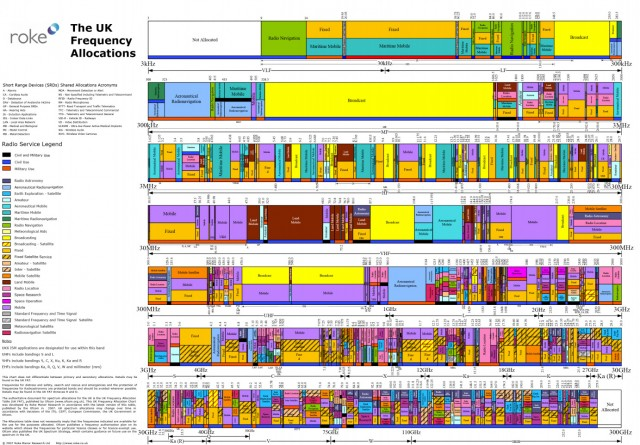
\includegraphics[height = 7 cm]{uk-spectrum-allocation-chart1-640x445.jpg}
\caption{A digram of current Spectral allocation \cite{Strategy2013}}
\label{spectrumalloc}
\end{figure*}

However, a closer inspection of the frequency allocation suggests this scarcity is artificial, it's more a product of regulatory oversight over time. As the constraints on spectrum requirement became more complex, so did the solutions to that problem - at the cost of leaving much of the spectrum idle for most of the time. 

For example: much of the spectrum is allocated to TV broadcast, radio broadcast and mobile. However, if we look closer, the allocations aren't even for specific companies - they're simply categories. Within these, OFCOM may have many licensees within each category.

Also interesting to note is how much frequency the Government allocates to itself (the red bar underneath the blocks indicates Government use). Compare this to the actual utilisation of spectrum: much of it is not used at all. Figure \ref{frequtil} shows a snapshot of frequency utilisation in three diverse locations in the UK over te radio specturm, note that many frequencies are not utilised (coloured blue) whilst others have significant activity (coloured yellow). Note that the plot for Southwark (central London) is barely different from Braddock - a rural area. 

\begin{figure*}[h]
\centering
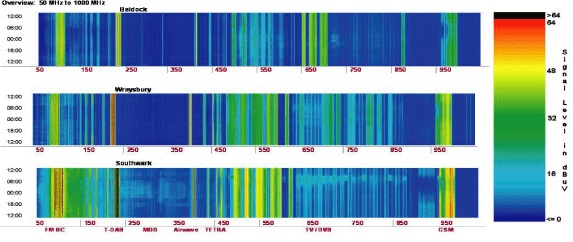
\includegraphics[height = 7 cm, width=0.5\textwidth]{cr2.jpg}
\caption{A snapshot of frequency utilisation in various areas: many frequencies are not used at all, whilst there is significant activity on others \cite{Burbidge2007}}
\label{frequtil}
\end{figure*}

How do we then go about solving this issue - how can we obtain the most significant bits of information from our sensing mechanism, whilst obviating the need to compress the data once we are done? How do we dynamically assign spectrum? The work of Candes, Tao \cite{Candes2006} and Donoho \cite{donoho2}, has shown that instead of measuring the information we require directly (and then compressing it), we can measure 'holographic' and non-linear random projections between our measurement space and the space where our data is sparse. This requires only the knowledge that the signal is compressible via some transform - both the acquisition protocol and the reconstruction algorithm are agnostic to the type of signal. What is surprising is that the sampling kernels are fixed independently of the signal, are non-adaptive and these projections are sufficient to reconstruct the signal - as if we had an Oracle to tell us where the non-zero components of our signal are. 

This work has had a large impact in medical imaging since it's inception: for example, it's now possible to take an image of a patient's heart within a single breath, as well as dynamic imaging of the heart (\cite{Donoho} figures 7 and 9).

Modern digital signal processing techniques (such as modulation techniques) are far more spectrally efficient than their historic analogue counterparts, which has in part contributed to the spectrum crisis. All this is changing though: from the beginning of 2013 all TV in the UK will transmitted digitally. Historically, television in the UK was broadcast using analogue signals requiring 32 multiplexes. Digital TV requires 6 multiplexes, on the other hand. 

This freeing up of TV frequencies represents an opportunity: these frequencies have good propagation characteristics (they suffer less with free space path loss relative to higher frequencies), whilst sill providing good bandwidth for data transmission. These TV frequencies are being opened up to civilian and  commercial users: spectral holes will be able to be exploited opportunistically by devices, so long as they don't interfere with the reception of TV. Historically, this is the single largest gift of new spectrum, and because there is no requirement for licensing this spectrum is free.

As with all technological innovations, this will not only improve existing infrastructure but also new classes of devices to transmit, for instance; applications such as passive sensor networks) which only need spectrum intermittently to transmit monitoring results), inter-vehicle communication for real time traffic monitoring and wireless internet at broadband data rates have all been proposed.

Despite all of this hype, dynamic spectrum access won't become a reality unless spectral holes can be robustly detected. The requirement that secondary users exploit the new spectrum politely, without interference to primary user makes spectrum sensing essential to TV white-space (TVWS) technologies. The realisation of any Cognitive Radio standard (such as IEEE 802.22), requires the co-existence of primary (TV users) and secondary (everybody else who wants to use TVWS spectrum) users of the frequency spectrum to ensure proper interference mitigation and appropriate network behaviour. 

Users of TVWS (Cognitive Radios) must sense whether spectrum is available, and must be able to detect very weak primary user signals. Furthermore they must sense over a wide bandwidth (due to the amount of TVWS spectrum proposed), which challenges traditional Nyquist sampling techniques, because the sampling rates required are not technically feasible with current RF or Analogue-to-Digital conversion technology.

Sensing should enable devices to detect the presence of TV signals in a band and provide smart and adaptive (and possibly distributed) solutions to band identification.

Spectrum sensing should involve:

\begin{enumerate}
\item Sensing to detect white spaces.
\item Co-existence with similar devices.
\item Frequency monitoring of other devices.
\item Interference management. 
\item Spectrum mobility and transmission power control when needed.
\end{enumerate}

As described earlier, the available spectrum is highly underutilised, and can be thought of as a collection of narrowband transmissions over a wideband channel. As such, the spectrum we're sensing is sparse. This makes it an ideal candidate for sparse recovery techniques such as Compressive Sensing.  

The report is divided into three chapters: the remainder of this chapter describes methods for sensing narrowband signals (i.e. channels where the frequency response is approximately flat, and where the bandwidth is smaller than the coherence bandwidth of the channel), and the limitations of these are highlighted for the problem of sensing spectrum for Cognitive Radios. 

Classical and Compressive Sensing are then contrasted, including the main ideas such as incoherence and the Restricted Isometry Property, and illustrating the number of samples required for full reconstruction.   Somme approaches to solving the optimisation problems posed by the new framework are also discussed.

Chapter 2 introduces Group Testing, and covers new work which has been accepted for publication at Allerton 2014. After some preliminary remarks the Capacity of a Group Testing problem is defined. Then, previous work on variations of an algorithm by Hwang are discussed, including upper and lower bounds on Capacity. Finally, a new algorithm is presented along with an analysis of the average number of tests the algorithm will execute.

The focus of Chapter 3 is again compressive sensing, this time in a distributed setting - given a connected network of nodes, how can we organise sensing to reconstruct a wideband signal? The chapter begins by discussing various signal models in the literature, and justifies the use of a single model. Then the sensing model is presented as a multinode extension of the Modulated Wideband Converter (\cite{mishali2010theory}). There follows an extended discussion of constrained convex optimisation, and an introduction to the Alternating Direction Method of Multipliers. Finally, how to sense the requisite signals and use a distributed setup to solve the system is explained. Some tentative results of simulations are also presented.

\section{Classical Sensing}
Classically, for perfect signal reconstruction, we must sample a signal such that the sampling rate must be at least twice the maximum frequency in the bandlimited signal. The continuous time signal can then be recovered using an appropriate reconstruction filter (e.g. a sinc filter). For example, we can represent a sampled continuous signal as a multiplication of the signal with a train of Dirac delta functions at multiples of the sampling period T.
%

%
where
%


Working the frequency domain, this multiplication becomes convolution (which is equivalent to shifting):

\begin{equation}
\hat{X}_{s}\left(f\right) = \sum_{k=-\infty}^\infty x\left(t - kT\right)
\end{equation}

Thus if the spectrum of the frequency is supported on the interval \(\left(-B, B\right)\) then sampling at intervals \(\frac{1}{2B}\) will contain enough information to reconstruct the signal \(x(\left(t\right)\). Multiplying the spectrum by a rectangle function (low-pass filtering), to remove any images caused by the periodicity of the function, and the signal \(x(\left(t\right)\) can be reconstructed from its samples:

\begin{equation}
x\left(t\right) = \sum_{n=-\infty}^\infty x\left(nT\right) sinc\left(\frac{t_nT}{T}\right)
\end{equation}



\section{Narrowband Spectrum Sensing}

\subsection{Classical Spectrum Sensing}

\begin{definition}[Wide-sense Stationary Signal]
Given a (bandlimited) signal \(x\left(t\right)\), we say it is wide sense stationary, if the following conditions hold:

\begin{itemize}
\item
\begin{equation}
\ep{x\left(t\right)} = \mu \text{ } \forall t
\end{equation}
\item 
\begin{equation}
\ep{\left(x\left(t_1\right) - \mu\right)\left(x\left(t_2\right) - \mu\right)} = C_{x}\left(t_1 - t_2 \right) 
\end{equation}
\end{itemize}
i.e. the mean of the signal must be constant, and the autocovariance must depend only on the lag.
\end{definition}

From this we can define the power spectral density of the signal \(x\left(t\right)\):

\begin{definition}[Power Spectral Desnity]
\begin{equation}
S_{xx} \left(\omega\right) = \mid \hat{x}\left(\omega\right) \mid^2
\end{equation}
where \(\hat{x}\left(\omega\right)\) is the Fourier transform of \(x\left(t\right)\).
\end{definition}

\begin{definition}[Autcorrelation]
The autocorrelation of a signal \(R_{xx}\left(t_1, t_2\right)\) is defined as:

\begin{equation}
R_{xx}\left(t_1, t_2\right) = \ep{x\left(t-1\right)x\left(t_2\right)}
\end{equation}

For wide sense stationary signals, \( R_{xx}\left(t_1, t_2\right) = R_{xx}\left(t_1 - t_2,\right) = R_{xx}\left(\tau\right) \)

\end{definition}

The problem of spectrum sensing \cite{yucek2009survey} is to decide whether a particular band is available, or not. That is, we wish to discriminate between the following two hypotheses:

\begin{equation}
H_{0}: y\left[n\right] = w\left[n\right] \text{, n} =  1 \ldots N 
\end{equation}
\label{h1}

\begin{equation}
H_{1}: y\left[n \right] = x\left[n\right] + w\left[n\right] \text{, n} =  1 \ldots N 
\end{equation}
\label{h2}

Where \(x\) is the (deterministic) primary users signal, having a specific structure which stems from modern coding and modulation techniques, \(w\) is additive white Gaussian noise and \(y\) is the received signal.

Any detection strategy is a function, \(f: \re^n \rightarrow \{0,1\}\), mapping the output of sensing to \(\{0, 1\}\). ) means the received signal is noise, whilst 1 means that a Primary User signal is present.

To decide whether the observations \(\textbf{y}\) were generated under \(\textit{H}_{0}\) or \(\textit{H}_{1}\) is accomplished by forming a test statistic \(\Gamma\left(y\right)\) and then comparing this statistic with a predefined threshold \(\lambda\). Both classical methods, where the hypotheses are assumed to be deterministically true and the goal is to minimise the false detection probability, and Bayesian methods, where it is assumed that the source selects the true hypothesis at random according to some prior probabilities, agree that the test statistic should be likelihood ratio:

\begin{equation}
\Gamma\left(\textbf{y}\right) = \frac{p\left(\textbf{y}\mid H_0\right)}{p\left(\textbf{y}\mid H_1\right)}
\end{equation}

The performance of a detector is quantified in terms of the probability of detection

\begin{equation}
P_{D} = Pr\left( \Gamma\left(\textbf{y}\right) > \lambda \mid H_1\right)
\end{equation}

and the probability of false alarm 

\begin{equation}
P_{FA} = Pr\left( \Gamma\left(\textbf{y}\right) > \lambda \mid H_0\right)
\end{equation}

By varying \(\lambda\) the operating point of a detector can be chosen anywhere along its receiver operating characteristics curve.

There are several proposed spectrum sensing methods that enable cognitive radios identify bands and perform dynamic frequency selection. Some of the common (narrowband) spectrum sensing techniques are described below.

\subsubsection{Energy Detection}

Energy detection is the simplest form of spectrum sensing: this method simply compares the signal energy in a frequency band to a pre-defined threshold. If the threshold is exceeded the band is declared occupied. , This method is quite generic as receivers need no knowledge of the primary users signal, and in theory, this form of detection works irrespective of the type of Primary User signalling used. Energy detections is a common method for the detection of unknown signals in noise, due to low computational and implementation complexity. 

A typical implementation
 for energy detection would be to centre a bandpass filter on the band of interest, followed by a squaring device to measure the received energy and an integrator to determine the observation interval. Finally the output of the integrator is compared with a threshold to determine the presence of a signal. This threshold is determined based upon the noise variance of the channel. I.e. we have a decision metric of the following form:

\begin{equation}
M = \sum_{n=0}^N |y\left[n\right]|^2
\end{equation}

Modelling the signal and noise as zero-mean Gaussian random variables with variances \(\sigma_s\), and \(\sigma_n\) respectively, we can derive expressions for the metric, the detection probability and the false alarm probability \cite{yucek2009survey}

\begin{equation}
 M =
  \begin{cases}
   \frac{\sigma_w^2}{2} \chi^2_{2N} & H_0 \\
   \frac{\sigma_w^2 + \sigma_s^2}{2} \chi^2_{2N} & H_1
  \end{cases}
\end{equation}

\begin{equation}
P_D = 1 - \Gamma\left(1, \frac{\lambda}{1 + \frac{ \sigma_2^2 }{ \sigma_w^2 } } \right)
\end{equation}

\begin{equation}
P_FA = 1 - \Gamma\left(1, \frac{\lambda}{\sigma_w^2} \right)
\end{equation}

Where \( \Gamma\left(1,x\right)\) is the incomplete gamma function. From these equations it's clear to see that the performance of energy detection based sensing faces challenges at low SNR values. See \cite{yucek2009survey} figure 3 for curves quantifying the performance. 

Also energy detectors perform poorly under extreme fading conditions as they are unable to distinguish primary users and noise. Further this type of detector is not efficient at detecting spread spectrum signals. 

For energy detection we wish to maximise \(P_D\) subject to a constraint on \(P_{FA}\). This is done via a threshold \(\lambda\), which trades off these two probabilities.

Choosing \(\lambda\) requires knowledge of the Primary User transmissions, as well as estimates of the noise power. Given these, calculating the optimal \(\lambda\) is straightforward \cite{xie2009optimal}. Estimating the PU power is dependent on the radio environment between the PU transmitter and the CR. Noise power estimation isn't flawless and a small noise power estimation error can cause significant performance loss \cite{hamdi2010impact}, \cite{sahai2004some}.

Noise power uncertainty can be mitigated by using an adaptive algorithm \cite{zhang2011adaptive}, or an a variant of the MUSIC algorithm which separates signal and noise subspaces \cite{olivieri2005scalable}. These significantly increase the complexity of the energy detector, making it less attractive relative to other methods.

A more serious concern for energy detection is the SNR wall \cite{tandra2008snr}: an SNR below which an energy detector will fail to detect the presence of a PU signal no matter how long the detector observes the channel. This is because at low SNRs the PU signal is no longer well separated from the noise. There has been some work in overcoming this wall using cross correlation between multiple antennas \cite{oude2011lowering}.


\subsubsection{Cyclostationary Feature Detection}
Because the signals used in practical communication systems contain distinctive features that can be exploited for detection, it is possible to achieve a detection performance which substantially surpasses the energy detector \cite{ye2007spectrum}, \cite{kim2007cyclostationary}. This is in contrast to the predictions of information theory where maximum entropy signals will be statistically white and Gaussian (if this were the case, then we could do no better than the energy detector). More importantly, known signal features can be exploited to estimate unknown parameters such as noise power. 

Examples of well known patterns include pilot signals and spreading sequences. Other examples include preambles and midambles: known sequences transmitted before and in the middle of each slot, respectively. Others include redundancy added by coding, modulation and burst formatting used by the transmitter. 

This method exploits cyclostationary features of received signals: man made periodicity in the signal (for example symbol rate, chip rate, cyclic prefix etc) or its statistics - mean, autocorrelation. A cyclic correlation function is used instead of PSD (or autocorrelation sequence) for detecting signals present in a given spectrum. This is able to differentiate noise from primary users signals since noise is wide-sense stationary with no correlation but modulated signals are cyclostationary due to the redundancy of signal correlations. 

For clarity, the random processes encountered by a cognitive radio will have a period in both expectation and autocorrelation:

\begin{equation}
\mathbb{E}\left(t\right) = \mathbb{E}\left(t + mT\right) = \mathbb{E}\left[x\left(t\right)\right]
\end{equation}

\begin{equation}
\mathbb{R}\left(t, \tau\right) = \mathbb{R}\left(t + mT, \tau\right) = \mathbb{E}\left[x\left(t\right)\conjugate{x\left(t_+\tau\right)}\right]
\end{equation}

where \(t\) is time, \(\tau\) is the autocorrelation lag, \(x\left(t\right)\) is the random process we are considering and \(m\) is an integer. 

Due to the periodicity of the autocorrelation, it can be expressed as a Fourier series over integer multiples of the fundamental frequency in the signal as well as integer multiples of sums and differences of this frequency:
%
\begin{equation}
\mathbb{R}\left(t, \tau\right) = \sum_{\alpha} r\left(\alpha, \tau\right) e^{2\pi j \alpha t}  
\end{equation}
\label{cyclic-covarience}
%
with Fourier coefficients:
%
\begin{equation}
r\left(\alpha, \tau\right) = \frac{1}{T} \int_{T} x\left(t+\frac{\tau}{2}\right)\conjugate{x\left(t+\frac{\tau}{2}\right)} e^{-2\pi j \alpha t} dt
\end{equation}
%
where \(\alpha\) is the cyclic frequency

From this we can define the Cyclic Power Spectrum of the signal:

\begin{equation}
S\left(f\right) = \int_{-\infty}^{\infty} r\left(\alpha, \tau\right) e^{-2 \pi j f \tau} d\tau
\end{equation}

For a fixed lag \(\tau\), \ref{cyclic-covarience} can be re-written as:
%
\begin{equation}
R_{xx}\left(t, \tau \right) = R_{xx}\left(\tau\right) + \sum_{\alpha} r\left(\alpha, \tau\right) e^{2\pi j \alpha t}  
\end{equation}
%
i.e. a part dependent on the lag only (the cyclic frequency is zero), and a part which is a periodic function of time. 

Under both hypotheses, (\ref{h1}, \ref{h2}), the continuous portion of the signal exists, but the cyclo-stationary portion only exists under \ref{h2} when \(\alpha \neq 0\). Thus we only need to test for the presence of a cyclo-statrionary component. 

To this end re-write the hypotheses as:

\begin{equation}
H_{0}: y\left[n\right] = S_{w}^\alpha \left[n\right] \text{, n} =  1 \ldots N 
\end{equation}
\label{c1}

\begin{equation}
H_{1}: y\left[n \right] = S_{x}^{\alpha} \left[n\right] + S_{w}^{\alpha} \left[n\right] \text{, n} =  1 \ldots N 
\end{equation}
\label{c2}

where \(S_{x}^{\alpha}\) is the CPS of white noise which is zero for \(\alpha \neq 0 \).  Using the test statistic:

\begin{equation}
\chi = \sum_{\alpha \neq 0} \sum_{n} S_{x}^{\alpha} \conjugate{S_{x}^{\alpha}}
\end{equation}

we can formulate the cyclo-stationary detector as:

\begin{equation}
 d =
  \begin{cases}
   0 & \chi < \lambda  \\
   1 & \chi \geq \lambda
  \end{cases}
\end{equation}

where \(\lambda\) is some pre-determined threshold \cite{Ghozzi2006}. 

The advantages of this type of sensing over energy detection, are that its possible to distinguish primary user transmissions (as well as distinguish between different PU signals) \cite{lunden2007spectrum}. It is also possible to distinguish noise from PU signals as the noise spectrum has no cyclic correlation \cite{cabric2004implementation}, \cite{vcabric2005physical}. However, cyclic frequencies have to be assumed to be known \cite{Ghozzi2006}. 

\subsubsection{Matched Filtering}
If all the probability distributions and parameters  - noise variance, signal variance, channel coefficients etc - are known under both hypotheses, and the signal to be detected is perfectly known then the optimal test statistic is a matched filter \cite{cabric2004implementation}, \cite{yucek2009survey}.

A matched filter is the convolution of a test signal with a template signal (or window) and detects the presence of the template in the unknown signal (as the convolution measures the overlap of two signals).

For example: for a given TV signal, \(r\left(t\right)\) defined over \(0 \leq t \leq T\) the corresponding matched filter is \(h\left(t\right) = r\left(T - t\right)\). 

A test statistic can be formed by sampling the output of the filter every \(nT\) seconds and choosing \ref{h1} if the statistic is below some threshold and \ref{h2} otherwise.

When compared to other methods, matched filtering takes a shorter time to achieve a threshold probability of false alarm. However, matched filtering requires that radios demodulate received signals, and so requires perfect knowledge of primary users signalling features. Matched filtering also requires a prohibitively large power consumption, as various algorithms need to be executed for detection.

The paper \cite{bhargavi2010performance}, compares the performance of Energy Detection, Matched Filtering and Cyclostationary detection. It concludes that cyclostationarity based detection has the best performance (based on a lower \(P_{FA}\) for a given \(P_D\)), as this for of detection is naturally insensitive to noise uncertainty as the test statistic for cyclic detection doesn't require knowledge of the noise variance.

\subsection{Distributed Approaches to Spectrum Sensing}

\subsubsection{Limitations}
The methods described above, are appropriate for sensing whether a single channel is available for transmission, based upon the result of measurements of that channel. However, Cognitive Radios aim to exploit spectral holes in a wide band spectrum (i.e. a channel whose frequency response is not flat over the bandwidth) and will usually have to make a decision regarding transmission from measurements from this type of channel.

There are two proposed approaches to this: Multiband sensing and Compressive Sensing. Multiband sensing splits the wideband spectrum into a number of independent (not necessarily contiguous) sub-channels (whose frequency response is flat), and performs the hypothesis test for each sub-channel. However, in practice, there are correlations across sub-channels that this method fails to address. For example, digital TV signals are transmitted as spread spectrum signals so that primary user occupancy is correlated across channels. A related issue is that noise variance could be unknown but correlated across bands. Binary hypothesis testing then fails in this case, needing to be replaced by composite hypothesis tests which grow exponentially with the number of sub-channels. Such problems are typically non-convex and require prohibitively complex detectors.


\section{Introduction}

There is an almost ubiquitous growing demand for mobile and wireless data, with consumers demanding faster speeds and better quality connections in more places. Consequently 4G is now being rolled out in the UK and US and with 5G being planned for 2020 and beyond \cite{Dahlman2014}.  

However, there is constrained amount of frequencies over which to transmit this information; and demand for frequencies that provide sufficient bandwidth, good range and in-building penetration is high.

Not all spectrum is used in all places and at all times, and judicious spectrum management, by developing approaches to use white spaces where they occur, would likely be beneficial.

Broadly, access to spectrum is managed in two, complementary ways, namely through licensed and licence exempt access. Licensing authorises a particular user (or users) to access a specific frequency band. Licence exemption allows any user to access a band provided they meet certain technical requirements intended to limit the impact of interference on other spectrum users.

A licence exempt approach might be particularly suitable for managing access to white spaces. Devices seeking to access white spaces need a robust mechanism for learning of the frequencies that can be used at a particular time and location. One approach is to refer to a database, which maps the location of white spaces based on knowledge of existing spectrum users. An alternative approach is for devices to detect white spaces by monitoring spectrum use. 

The advantages of spectrum monitoring \cite{akan2009cognitive} over maintaining a database of space-frequency data are the ability of networks to make use of low-cost low-power devices, only capable of making local (as opposed to national) communications, keeping the cost of the network low and  opportunistic channel usage for bursty traffic, reducing channel collisions in dense networks.

The realisation of any Cognitive Radio standard (such as IEEE 802.22 \cite{stevenson2009ieee}), requires the co-existence of primary (e.g. TV users) and secondary (everybody else who wants to use TVWS spectrum) users of the frequency spectrum to ensure proper interference mitigation and appropriate network behaviour. We note, that whereas TVWS bands are an initial step towards dynamic spectrum access, the principles and approaches we describe are applicable to other frequency bands - in particular it makes ultra-wideband spectrum sensing possible.

The challenges of this technology are that Cognitive Radios (CRs) must sense whether spectrum is available, and must be able to detect very weak primary user signals. Furthermore they must sense over a wide bandwidth (due to the amount of TVWS spectrum proposed), which challenges traditional Nyquist sampling techniques, because the sampling rates required are not technically feasible with current RF or Analogue-to-Digital conversion technology.

Due to the inherent sparsity of spectral utilisation, Compressive Sensing (CS) \cite{Candes2006} is an appropriate formalism within which to tackle this problem. CS has recently emerged as a new sampling paradigm allowing images to be taken from a single pixel camera for example. Applying this to wireless communication, we are able to reconstruct sparse signals at sampling rates below what would be required by Nyquist theory, for example the works \cite{mishali2010theory}, \cite{Mishali2010a}, \cite{Mishali2009}, \cite{Mishali2011}, and \cite{tropp2010beyond} detail how this sampling can be achieved. 

However, even with CS, spectrum sensing from a single machine will be costly as the proposed TVWS band will be over a large frequency range (for instance in the UK the proposed TVWS band is from 470 MHz to 790 MHz, requiring traditional sampling rates of \textasciitilde 600 MHz). CS at a single sensor would still require high sampling rates. In this report we propose a distributed model, which allows a sensing budget at each node far below what is required by centralised CS.

\section{Wideband Spectrum Sensing}
This section presents a new method of sensing sparse signals, and its application to the problem of sensing over wideband spectra in Cognitive Radios. Initially we introduce Classical Sensing and then give an overview of both Compressive Sensing and Group Testing. Finally, we discuss some sub-Nyquist sampling techniques.

\begin{figure*}[h]
\centering
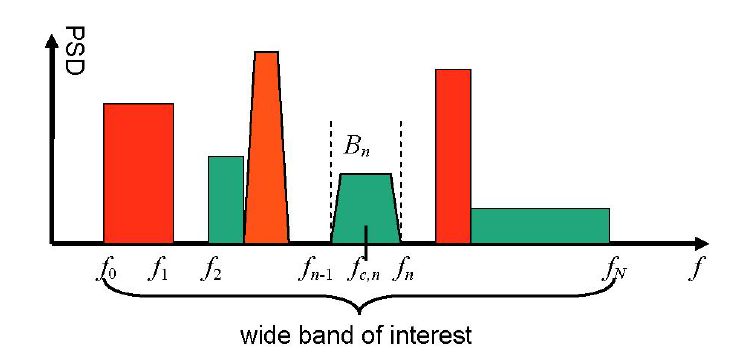
\includegraphics[height = 7 cm]{bands.png}
\caption{A digram of the Spectrum Sensing model \cite{Tian}}
\label{widebandspectra}
\end{figure*}

\subsection{Compressed Sensing}

Compressive sensing is a modern signal acquisition technique in which randomness is used as an effective sensing strategy for classes of signals typically encountered in practice.

Informally, CS posits that for \(k\)-sparse signals \(\in \re^{n}\) - signals with \(k\) non-zero amplitudes at unknown locations) - \(k\log{n}\) measurements are sufficient to exactly reconstruct the signal. In other words we can sample at the information rate, without information loss.

For TVWS signals, this reasoning can be inverted: signals with very large bandwidth - but with a sparse spectrum - can be sampled randomly in time at rates below below those thought sufficient by the Nyquist theorem.

This work has been extended to cases where the signal isn't exactly sparse, and where the measurements are imperfect.

The central idea of CS is that randomness is an effective sensing strategy. We require that sensing vectors satisfy two technical conditions (described in detail below): an Isotropy property, which means that components of the sensing vectors have unit variance and are uncorrelated, and an Incoherence property, which means that sensing vectors are almost orthogonal. These conditions are summed up in the Restricted Isometry Property.

Once the set of measurements have been taken, the signal may be reconstructed from a simple linear program.

In practice many signals encountered 'in the wild' can be fully specified by much fewer bits than required by the Nyquist sampling theorem. This is either a natural property of the signals, for example images have large areas of similar pixels, or as a conscious design choice, for example training sequences in communication transmissions. These signals are not statistically white, and so these signals may be compressed (to save on storage). For example, lossy image compression algorithms can reduce the size of a stored image to about 1\% of the size required by Nyquist sampling. 

Whilst this vein of research has been extraordinarily successful, it poses the question: if the reconstruction algorithm is able to reconstruct the signal from this compressed representation, why collect all the data in the first place, when most of the information can be thrown away? Is it possible to directly measure the part that will not end up being thrown away?

Compressed Sensing answers these questions, by way of providing an alternative signal acquisition method to the Nyquist theorem. Specifically, situations are considered where fewer samples are collected than traditional sensing schemes. 

That is, in contrast to Nyquist sampling, Compressive Sensing is a method of measuring the informative parts of a signal directly without acquiring unessential information at the same time. 

Signals which are compressible, are signals whose information content is smaller than the ambient dimension they are acquired in. Such signals have representations in which they are sparse (i.e. the most of the co-efficients in that representation are zero, or close to zero). For example, 

\begin{enumerate}
\item  A sine wave at frequency \(\omega\) is defined as a single spike in the frequency domain yet has an infinite support in the time domain
\item An image will have values for every pixel, yet the wavelet decomposition of the image will typically only have a few non-zero coefficients
\end{enumerate} 

We may not be able to directly obtain those coefficients, as we may not posses an appropriate measuring device or one may not exist, or there is considerable uncertainty about where the non-zero coefficients are. Yet we still are able to measure correlations between the signal and some waveforms \(\phi_{k}\) i.e. 
%
\begin{equation}
y_{k} = \left\langle f \text{,} \phi_{k} \right\rangle \text{ } k = 1 \ldots m
\end{equation}
%
for \( f \in \mathbb{R}^n \) expanded in an orthonormal basis \( \psi \) s.t.
%
\begin{equation}
f(t) = \sum_{i = 1}^n x_{i}\psi_{i}(t) 
\end{equation}
%
where the \(x_{i} \) are the coefficient sequence of f. 

%An example of a practical Compressive Sensing system is the single-pixel camera at Rice University \cite{Duarte2008}. Typical camera devices obtain pixel samples by exposing a bank of photon detectors (one for each pixel) to the incident light field. This data is the processed into an image.

%The single pixel camera takes pictures by first directing the incoming light field onto an array of tiny mirrors (one for each pixel). Each mirror can be either be oriented towards a single photon detector, or oriented away from the detector. In this setup, a measurement is taken as the sum of all the incident light beams. Afterwards, the mirrors are flipped to a new random configuration, and another measurement is taken. This process is repeated, until enough information has been collected to reconstruct the image. Figure \ref{singlepixelcamera} shows the operation of the single pixel camera.

%\begin{figure*}[h]
%\centering
%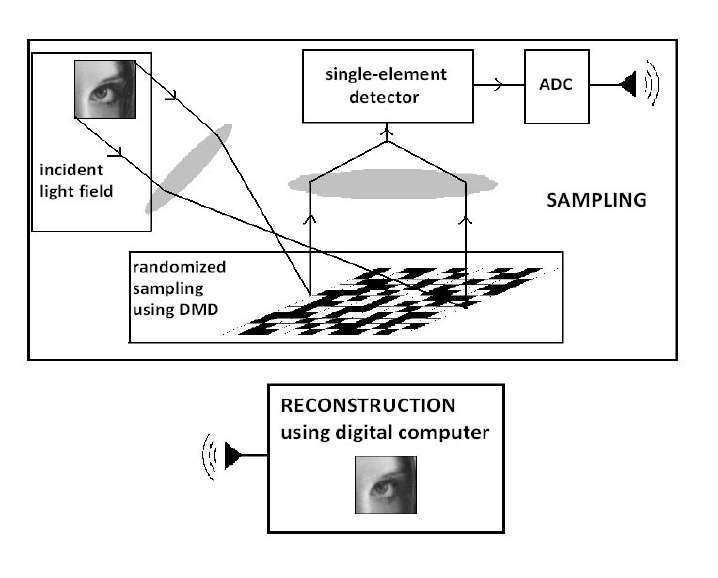
\includegraphics[height = 7 cm]{singlepixel.png}
%\caption{The operation of the single pixel camera at Rice University \cite{singlepixelimaging}}
%\label{singlepixelcamera}
%\end{figure*}

%Compressive Sensing works best if the \(x_{i}\) are compressible (i.e. they are distributed according to a power law), and the error \(\|x - x_{s}\|\) is small.

%In Compressive Sensing measurements are taken is an incoherent basis, as opposed to the basis of the original signal. 

Given that we know a basis in which our signal is sparse, \(\phi\), how do we choose \(\psi\), so that we can accomplish this sensing task? In classical sensing, we choose \(\psi_k\) to be the set of \( T_s \)-spaced delta functions (or equivalently the set of \( 1/T_s \) spaced delta functions in the frequency domain). A simple set of \(\psi_k\) would be to choose a (random) subset of the delta functions above.

In general, we seek waveforms in which the signals' representation would be dense.

\begin{defn}
A pair of bases is said to be incoherent if the largest projection of two elements between the sensing (\(\psi\)) and representation (\(\phi\)) basis  is in the set \( [1 , \sqrt{n}] \), where \( n \) is the dimension of the signal. 
\end{defn}

The coherence of a set of bases is denoted by \(\mu\).

This implies that sensing with incoherent systems is good (in the sine wave example above it would be better to sample randomly in the time domain as opposed to the frequency domain), and efficient mechanisms ought to acquire correlations with random waveforms (e.g. white noise).

\textbf{Theorem} \cite{Candes2006}
Fix a signal f \(\in \mathbb{R}^n\) with a sparse coefficient basis, \(x_{i}\) in \(\phi\). Then a reconstruction from \(m\) random measurements in \(\psi\) is possible with probability \(1 - \delta\) if: 

\begin{equation}
m \geq C \mu^2(\phi, \psi) S \log\left(\frac{n}{\delta}\right)
\end{equation}
\label{minsamples}

where \( \mu(\phi, \psi)\) is the coherence of the two bases, and \(S\) is the number of non-zero entries on the support of the signal.

Once we have obtained the measurements \(m\), we need to reconstruct the signal. 

To recover a sparse vector, we must make sure that the vectors are not in the null space of the sensing matrix (otherwise there would be no hope of recovery). We also require that any subset of \(S\) columns taken from the measurement matrix be nearly orthogonal w.r.t sparse vectors: i.e. all pairwise distances between S-sparse vecotrs be well preserved in the measurement space.

This can be summed up in the following inequality (Restricted Isometry Property) \cite{Emma}:

\begin{equation}
\left(1-\delta\right)\vectornorm{x}_{l_2}^2 \leq \vectornorm{Ax}_{l_2}^2 \leq \left(1+\delta\right) \vectornorm{x}_{l_2}^2
\end{equation}
\label{RIP}

We are also in a position to evaluate the meaning of the constant \(\mu\) in \ref{minsamples}. We are considering sampling within orthonormal systems (for example, Time and Frequency):
%
\begin{equation}
A*A = nI
\end{equation}
\label{orthonormal}
%
so that each row or column has \(l_2\) norm equal to \(sqrt{n}\). \(A\) is any matrix satisfying this property (examples include the Fourier matrix and the Dirac matrix). Thus \(\mu\) must be in the set \(\left[1, \sqrt{n}\right]\). \(\mu\) then, is a measure of how concentrated the rows of our measurement matrix is - i.e. how much information is spread across each vector. If \(\mu = 1\) then the rows are 'flat' -  and we need relatively fewer samples to reconstruct an S-sparse signal (i.e. each sample provides the same amount of information). However, if the rows contain all non-zero entries except for a single component, then \(\mu^2 = n\) and we will need to observe all components to determine the non-zero one (i.e. we have no guarantees of recovery from limited samples) \cite{Candes2007}. 

Noting that the measurements we take are projections from our orthonormal system (from example time) onto a sparsifying basis (i.e. frequency) we can see that:

\begin{equation}
\mu = max_{k,j} |\langle \phi_k, \psi_j \rangle |
\end{equation}
\label {mudef}
 
So we need to choose a sensing basis, where the vectors will be 'spread out', and the degree of spreading is characterised by \(\mu\).

The correct functional to minimise would be:

\begin{equation}
min\|\tilde{x}\|_{l_{0}} \text{ subject to } y_{k} = \langle \phi_{k} \text{,} \psi x^* \rangle \text{   } \forall k \in M \subset [1 \ldots n]
\end{equation}
\label{programl0}

where 

\begin{equation}
|| s ||_0 = |s|
\end{equation}

However, this norm is not convex and so minimising it is an NP-hard optimisation problem. As we are seeking sparse solutions the \(l_1\)-norm will suffice \cite{Donoho2006a}. This is because all vectors in a random \(k\)-dimensional subspace of an \(n\)-dimensional space are approximately Gaussian (in the sense that the components are distributed according to an approximate normal distribution). Such vectors have roughly equivalent norms, and so any solution to the \(l_1\) minimisation problem will be the same solution to the \(l_0\) minimisation problem for sufficiently sparse signals.

Thus the role of \(l_{1}\) minimisation is to decompress the data. There are many ways to perform this operation: some popular methods are basis pursuit \cite{Chen1998} and Greedy approaches such as Orthogonal Matching Pursuit \cite{Tropp2007}. 

Then \(f^*\) (the proposed reconstruction) is given by \(f^* = \psi x^*\) where \(x^*\) is the solution to the convex optimisation program (n.b. \(\| x\|_{l_{1}} := \sum_{i} |x_{i}| \)):

\begin{equation}
min\|\tilde{x}\|_{l_{1}} \text{ subject to } y_{k} = \left\langle \phi_{k} \text{,} \psi x^* \right\rangle \text{   } \forall k \in M \subset [1 \ldots n]
\end{equation}
\label{programl0}

In summary the \textbf{CS: Sample non-adaptively in an incoherent domain and invoke linear programming after the acquisition step to decompress the signal}

\subsection{RIPless Theory}


\subsubsection{Short, Fat matrices}
As remarked upon earlier: Compressive Sensing is equivalent to solving an under-determined linear system, with the constraint that we seek the sparsest solution. The content of the previous sections amounts to constraints on the number of rows of matrix of this linear system. 

If we had an Oracle which could tell us where the non-zero components of our solution were, then we would need only as many rows of the matrix as there were non-zero components in the signal to fully specify the problem. 

\begin{figure*}[h]
\centering
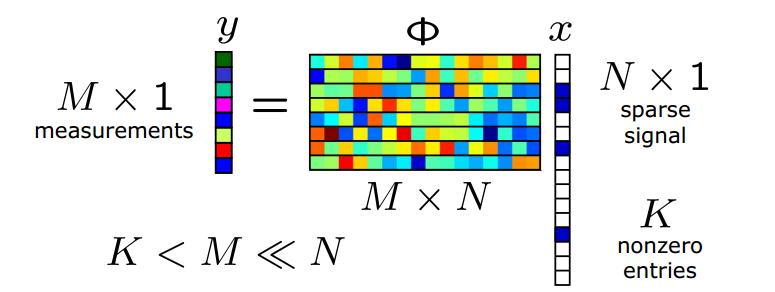
\includegraphics[height = 7 cm, width=\textwidth]{compressive_sensing_example.jpg}
\caption{A visualisation of the Compressive Sensing problem as an under-determined system}
\label{l1l2}
\end{figure*}

However, such and Oracle does not exist, and so we're left with the task of constructing a matrix to recover those components. Knowing that we're looking for k-sparse solutions, we need a matrix with at least 2k columns which are linearly independent. Equivalently, all images of \(k\)-sparse vectors under the operation of the sensing matrix \(\Phi\) must be distinct. From this, any k-sparse signal can be reconstructed from \(Ax\). 

To prove this assume the opposite - then there are two vectors \(x, x' \in \mathbb{R}^n\) such that \(Ax = Ax'\). I.e. \(A(x-x') = 0\). However, \((x-x')\) is 2k-sparse and so there is a linear dependence between 2k columns of the sensing matrix A. We have a contradiction, and so 2k columns will suffice to reconstruct a k-sparse signal. 

The problem with this is that we are trying to find the support of a k-sparse signal over a vector of length N, and so we would need to check all \(N \choose k\) combinations of k-sparse signals which is prohibitively computationally expensive. Is there some way to gain the advantages of sparsity, without having to minimise a non-convex functional?

As it turns out, the answer is yes. If we take \( m \geq C \mu^2(\phi, \psi) S \log\left(n\right) \) rows minimising the \(l_{1}\) norm will find the sparsest solution. This is because the \(l_1\) norm is an octahedron (in 3-dimensions, in higher dimensions it has an analogous spiky geometry), and solutions are more likely to intersect the norm at the points. Figure \ref{l1l2} shows this.

\begin{figure*}[h]
\centering
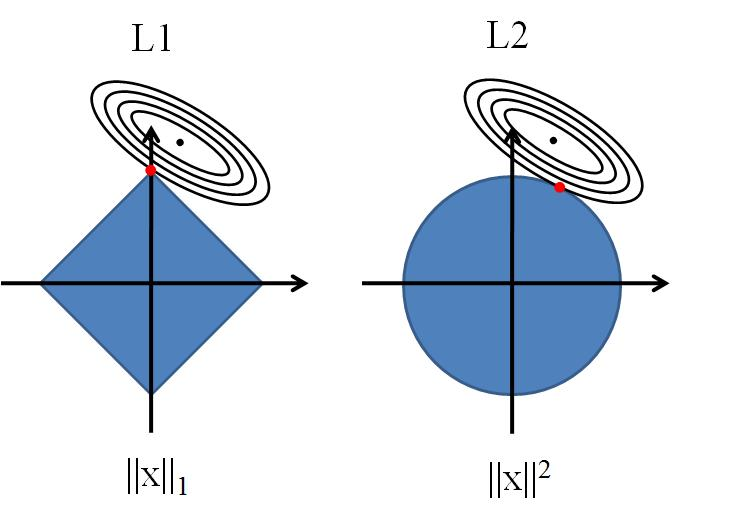
\includegraphics[height = 7 cm]{l1l2.jpg}
\caption{Solutions to the Compressive Sensing optimisation problem intersect the \(l_1\) norm the points where all components (but one) of the vector are zero (i.e. it is sparsity promoting) \cite{Tibshirani1996}}
\label{l1l2}
\end{figure*}

\subsubsection{Bayesian Compressive Sensing}
Based on the discussion above we can represent the compressive sensing measurements as: 

\begin{equation}
\textbf{g} = \Phi	\textbf{w}
\end{equation}

where \(\Phi\) is a \(K \times	N\) matrix which is the product of the measurement and sparse bases described earlier.

Note that the measurements may be noisy, with the measurement noise represented by a zero mean Gaussian distribution and unknown variance \( \sigma^2 \):

\begin{equation}
\textbf{g} = \Phi \textbf{w} + \textbf{n}
\end{equation}
\label{CSequation}

Where \textbf{n} is the vector representing the vector of noise, and has the same support as the measurements. 

Previous sections have shown how the weights \(w\) may be found through optimisation methods such as basis pursuit or greedy algorithms. Here, an alternative Bayesian model is described.

From \ref{CSequation} we have a Gaussian likelihood model: 

\begin{equation}
p \left( \textbf{g} \mid \textbf{w}\text{,} \sigma^2 \right) = (2 \pi \sigma^2)^{-K/2} \exp{\left(- \frac{1}{2 \sigma^2} \|\textbf{g} - \Phi	\textbf{w}\|_{2}^{2} \right)} 
\end{equation}

The above has converted the CS problem of inverting sparse weight \textbf{w} into a linear regression problem with a constraint (prior) that \textbf{w} is sparse. 

To seek the full posterior distribution over \textbf{w} and \( \sigma^2 \), we can chose a sparsity promoting prior. A popular sparseness prior is the Laplace density functions:

\begin{equation}
p\left(w\mid\lambda\right) = \left(\frac{\lambda}{2}\right)^N exp{-\lambda \sum_{i=1}^{N} |w_i|}
\end{equation}

Note that the solution the convex optimisation problem \ref{program0} corresponds to a maximum \textit{a posteriori} estimate for \(w\) using this prior. I.e this prior is equivalent to using the \(l_1\) norm as an optimisation function (see figure \ref{laplacenormal} \cite{Tibshirani1996}).

\begin{figure*}[h]
\centering
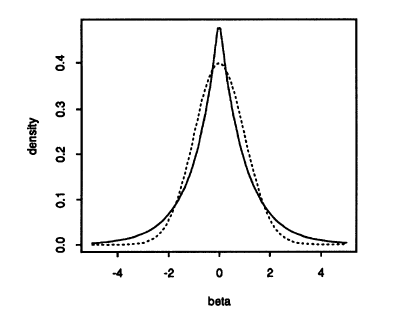
\includegraphics[height = 7 cm]{LaplaceandNormalDensity.png}
\caption{The Laplace (\(l_1\)-norm, bold line) and Normal (\(l_2\)-norm, dotted line) densities. Note that the Laplace density is sparsity promoting as it penalises solutions away from zero more than the Gaussian density. \cite{Tibshirani1996}}
\label{laplacenormal}
\end{figure*}

The full posterior distribution on \(w\) and \(\sigma^2\) may be realised, by using a hierarchical prior instead. To do this, define a zero-mean Gaussian prior on each element of \(w\):
%
\begin{equation}
p\left(w\mid a\right) = \prod_{i=1}^{N}\mathbb{N}\left(w_i\mid 0, \alpha_{i}^-1\right)
\end{equation}
%
where \(\alpha\) is the precision of the distribution. A gamma prior is then imposed on \(\alpha\):

\begin{equation}
p\left(\alpha \mid a, b \right) = \prod_{i=1}^{N} \Gamma\left( \alpha_i \mid a, b \right)
\end{equation}

The overall prior is found by marginalising over the hyperparameters:

\begin{equation}
p\left( w \mid a, b \right) = \prod_{i=1}^{N} \int_{0}^{\infty} \mathbb{N}\left(w_i\mid 0, \alpha_{i}^-1\right) \Gamma\left( \alpha_i \mid a, b \right)
\end{equation}

This integral can be done analytically and is a Student-t distribution. Choosing the parameters \(a,b\) appropriately we can make the Student-t distribution peak strongly around \(w_i = 0\) i.e. sparsifying. This process can be repeated for the noise variance \(\sigma^2\). The hierarchical model for this process is shown in \ref{bayesiancs}. This model, and other CS models which not necessarily have closed form solutions, can be solved via belief-propagation \cite{Baron2010}

\begin{figure*}[h]
\centering
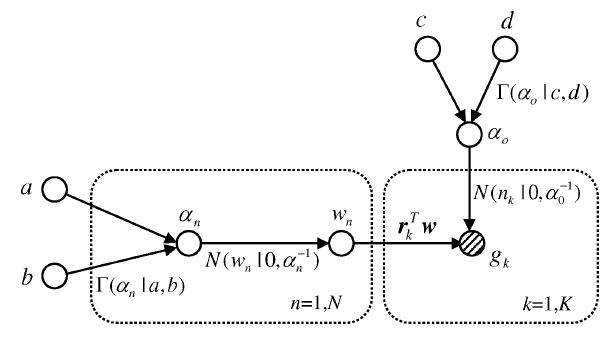
\includegraphics[height = 7 cm]{bayesiancs.png}
\caption{The hierarchical model for the Bayesian CS formulation \cite{Ji2008}}
\label{bayesiancs}
\end{figure*}


\subsection{Sub-Nyquist Sampling techniques}
This section presents some work on sampling methods for wide-band spectrum sensing

\subsubsection{Wideband Modulated Converter} 
The sampling scheme proposed in \cite{Mishali2010} is capable of sampling wideband signals at rates below those predicted by Shannon-Nyquist sampling theory. 

It works by mixing the incoming analogue signal \(x\left(t\right)\) with a mixing function \(p_i\left(t\right)\) aliasing the spectrum. \(x\left(t\right)\) is assumed to be bandlimited and composed of up to \(N_sig\) uncorrelated transmissions (i.e. possible narrowband channels). 

This process is repeated in parallel over \(M\) channels (unrelated to \(N_sig\) so that each band in \(x\) appears in baseband. The mixing functions are required to be periodic, with period \(T_p\). Since \(p_i\) is periodic it has Fourier expansion:

\begin{equation}
p_i\left(t\right) = \sum_{l=-\infty}^{\infty} c_{il} exp{jlt\frac{2\pi}{T_p}}
\end{equation}

The \(c_{il}\) are the Fourier coefficients of the expansion and are defined in the standard manner. The result of the mixing procedure in channel \(i\) is therefore \(xp_i\), with Fourier transform:

\begin{align}
X_{i}\left(f\right) &=& \int_{-\infty}^{\infty} x\left(t\right) p_i\left(t\right) dt
\\ &=& \sum_{l=-\infty}^{\infty} c_{il} X\left(f-lf_p\right)
\end{align}

\begin{figure*}[h]
\centering
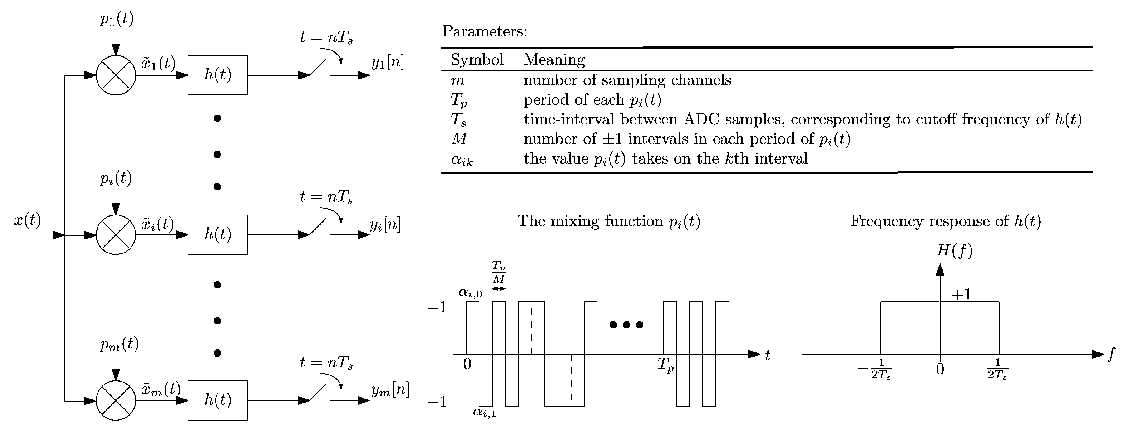
\includegraphics[height = 7 cm, width=\textwidth]{mwc.png}
\caption{The operation of the Modulated Wideband Converter \cite{mishali2010theory}}
\label{bayesiancs}
\end{figure*}

(insert the Fourier series for \(p_i\), then exchange the sum and integral). The output of this mixing process then, is a linear combination of shifted copies of \(X\left(f\right)\), with at most \(\lceil f_NYQ/f_p\rceil\) terms since \(X\left(f\right)\) is zero outside it's support (we have assumed this Nyquist frequency exists, even though we never sample at that rate).

Once the mixing process has been completed the signal in each channel is low-pass filtered and sampled at a rate \(f_s \geq f_p\). In the frequency domain this is a ideal rectangle function, so the output of a single channel is:

\begin{equation}
Y_i\left(e^{j 2 \pi f T_s }\right) = \sum_{l = -L_0}^{+L_0}
\end{equation}

since frequencies outside of \([-f_2/2, f_s/2]\) will filtered out. \(L_0\) is the smallest integer number of non-zero contributions in \(X\left(f\right)\) over \([-f_2/2, f_s/2]\) - at most \(\lceil f_NYQ/f_p\rceil\) if we choose \(f_s = f_p\). These relations can be written in matrix form as:

\begin{equation}
\textbf{y} = \textunderscore{\textbf{A}}\textbf{x}
\end{equation}

where \(\textbf{y}\) contains the output of the WMC process, \(\textunderscore{\textbf{A}}\) contains the Fourier coefficients of the mixing functions, and \(\textbf{x}\) is the vector of unknown samples of \(x\left(t\right)\). 

\section{Results and Simulations}
To compare the efficacy of Group Testing and Compressive Sensing, Hwang's algorithm and the algorithm presented in \cite{Aldrouobi} were simulated for a problem size of N=1024 and K=10.  The problem was simulated 100 times and the cumulative distribution found - i.e. after how many tests or measurements were the respective problems solved? This allows the number of tests required by Group Testing to be compared to the number of measurements in Compressive Sensing. Figure \ref{GTvsCS} shows the results:

\begin{figure*}[h]
\centering
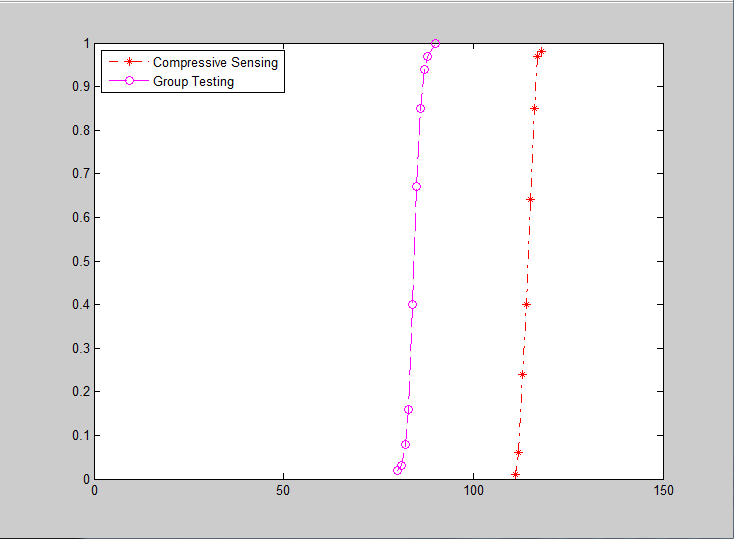
\includegraphics[height = 7 cm]{GTvsCS.png}
\caption{Group Testing vs Compressive Sensing}
\label{GTvsCS} 
\end{figure*}

Note that both the algorithms meet their respective asymptotic bounds (\( \log_2{N \choose K}\) in the case of GT and \(k\log{N}\) for CS). The main point of interest is that Group Testing requires roughly \(\frac{2}{3}\) of the tests required by Compressive Sensing. This is encouraging: despite there being 'less' information - in the sense that the result is a binary number as opposed to a real one -  GT outperforms CS. Intuitively, one would conjecture the opposite - more information should allow you to locate the non-zero components faster. This justifies our interest in the problem, as the performance increase is substantial. 


The contributions of this report are that we propose a distributed model and solver pair which obviates the need for a Fusion Centre (centralised node) as in \cite{Zhang2011b}) to do any data processing. That is the solution is found in a distributed manner, by local computations and communications in with one-hop neighbours. This can be applied to other models which previously required central processing.

Moreover, our algorithm is simple to understand (it is an extension of the multi-block ADMM \cite{mota2013d}) and can be applied to other composite optimisation problems.

We also give new proofs of ideas found in \cite{mota2013d}. 

The structure of the report is as follows: in section \ref{sec:sensingmodel} we introduce the sensing model, in section \ref{sec:opt-on-graphs} we describe the distributed reconstruction algorithm \cite{mota2013d}, and finally in section \ref{sec:results} we show some results of the reconstruction quality of this model. 




\section{Constrained Optimisation on Graphs}\label{sec:opt-on-graphs}

We model the network of sensors as an undirected graph \(G = \left(V,E\right)\), where \(V = \{1 \ldots J\}\) is the set of vertices, and \(E = V \times V\) is the set of edges. An edge between nodes \(i\) and \(j\) implies that the two sensors can communicate. The set of nodes that node \(i\) can communicate with is written \(\mathcal{N}_i\) and the degree of node \(i\) is \(D_i = |\mathcal{N}_i|\). 

Individually nodes make the following measurements (as discussed in section \ref{sec:sensingmodel}):

\begin{equation}
\vec{y}_p = \vec{A}_p\vec{x} + \vec{n}_p
\end{equation}

where \(\vec{A}_p\) is the \(p^{th} \) row of the sensing matrix from \eqref{system}, and the system \eqref{system} is formed by concatenating the individual nodes' measurements together.

We assume that a proper colouring of the graph is available: that is, each node is assigned a number from a set \(C = \{1 \ldots c \} \), and no node shares a colour with any neighbour. This is so that nodes may communicate in colour order, as opposed to communicating individually thus reducing the total number of communication rounds required. 

To find the \(\vec{x}\) we are seeking (the solution to the linear system, \ref{system}), to each node we give a copy of \(\vec{x}, \vec{x}_p\) and we constrain the copies to be identical across all edges in the network. Each node, thus has a separate optimisation to solve, subject to the constraint that it is consistent with its neighbours.

The problem then is to solve:

\begin{align}
\argmin_{\bar{x}} \sum_{c=1}^C \sum_{j \in c} f\left(x_j\right) + \frac{\lambda}{J} g\left(x_j\right) \nonumber \\ 
\text{ and } x_i = x_j \text{ if } \{i,j\} \in E \nonumber \\
\text{ and } x_i = z_i \text{ } \forall i \in \{1, \ldots, C\}
\label{constrainedbp}
\end{align}

with a particular special case being:

\begin{align}
\argmin_{\bar{x}} \sum_{c=1}^C \sum_{j \in c} \|A_jx_j - y_j\|_2^2 + \frac{\lambda}{J}\|z\|_1 \nonumber \\ 
\text{ and } x_i = x_j \text{ if } \{i,j\} \in E \nonumber \\
\text{ and } x_i = z_i \text{ } \forall i \in \{1, \ldots, C\}
\label{constrainedbp}
\end{align}

i.e. \(f = \vectornorm{x}_2^2\) and \(g = \vectornorm{x}_1\).

That is, at each node we minimise a Lasso functional constrained to be consistent across edges but that is separable in the \(l_2\) and \(l_1\) norms.

We can write the global optimisation variable as \(\bar{x}\), which collects together \(C\) copies of a \(n\times 1\) vector \(\vec{x}\):

\begin{defn}
We define vectors \(x_c\), where \(c = 1,\ldots , C\) and write the vector of length \(nJ\):
\begin{equation}
\bar{x} = \sum_{c=1}^C w_c \otimes x_c = \left[x_{c(1)}^T, \ldots	, x_{c(J)}^T\right]^T
\label{barxc}
\end{equation}
where \(w_{c(i)} = \mathbb{I}(c(i) = c)\), \(\mathbb{I}\) is the indicator function, and we have written \(c(i)\) for the colour of the \(i\)th node.
\end{defn}

These constraints can be written more compactly by introducing the node-arc incidence matrix B: a \(V\) by \(E\) matrix where each column is associated with an edge \(\left(i,j\right) \in E\) and has \(1\) and \(-1\) in the \(ith\) and \(jth\) entry respectively. Figures \eqref{efig:ex-network} and \eqref{fig:incidence-matrix} show examples of a network and it's associated incidence matrix.

The constraint \(x_i = x_j \text{ if } \{i,j\} \in E \) can now be written 

\begin{equation}
\sum_{c=1}^C\left(B_c^T \otimes I_n\right)\bar{x}_c = 0
\label{compact-constraints}
\end{equation}

note that \(\left(B^T\otimes I_n \right) \in \re^{nE \times nJ}\). Together \eqref{barxc} and \eqref{compact-constraints}, suggests that the problem \eqref{constrainedbp} can be re-written as:

\begin{align}
\argmin_{\bar{x}} \sum_{c=1}^C \sum_{j \in C_c} f\left(x_j\right) + \frac{\lambda}{J} g\left(z_j\right)
\nonumber \\
\text{ s.t. } \sum_{c=1}^C\left(B_c^T \otimes I_n\right)\bar{x}_c = 0 \nonumber \\
\text{ and } \bar{x}_c - \bar{z}_c = 0
\label{constrainedbp1}
\end{align}

where \(\beta = \frac{\lambda}{J}\).

The global Augmented Lagrangian \cite{Boyd2010a}
 for the problem \eqref{constrainedbp1} can be written down as:

\begin{align}
L_\rho = \sum_{c=1}^C  ( \sum_{j \in c} & f\left(x_j\right) + \frac{\lambda}{J} g\left(z_j\right)  + \nonumber \\ & + \theta^T\left(\bar{x}_j - \bar{z}_j\right)  +  \frac{\rho}{2}\vectornorm{\bar{x}_j-\bar{z}_j}_2^2 ) + \nonumber \\  & + \eta^T\left(B_c^T \otimes I_n\right)\bar{x}_c + \frac{\rho}{2}\vectornorm{\sum_{c=1}^C\left(B_c^T \otimes I_n\right)\bar{x}_c}_2^2
\label{aug-lagrange}
\end{align}

This is, superficially, similar to the Augmented Lagrangian for the Lasso problem \cite{Boyd2010a}[Section 6.4]. That is, the terms indexed by \(j\) are a straightforward Lasso problem, constrained by edge-wise variables (indexed by \(c\)) forcing consistency across the network. However, the problem (as currently written) is not separable across the edges of the network as the final and penultimate term represent the constraint that the nodes agree on their estimates across edges. 

To make it possible that \ref{aug-lagrange} can be posed  as a constrained optimisation problem at each node, we introduce the following variable (so that the the final term of \ref{aug-lagrange} is separable across edges of the graph):

\begin{defn}
\begin{align*}
u &:= \left(B^T \otimes I_n\right)\bar{x} \\
& = \left(B^T \otimes I_n\right)\sum_{c=1}^C w_c \otimes x_c \\
& = \sum	_{c=1}^C B_c^T\otimes x_c
\end{align*}
where we have used the definition \eqref{barxc} in the second line, and the property of Kronecker products \((A\otimes C)(B \otimes D) = (AB \otimes CD)\) between the second and third lines, and we write \(B_c = w_c^TB\).
\end{defn}

\begin{figure}[h]
\centering
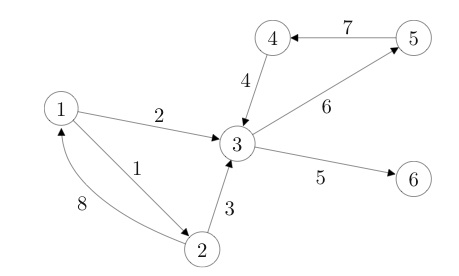
\includegraphics[height = 5 cm]{network-ex-incidence-mat.jpg}
\caption{An example of a network}
\label{efig:ex-network}
\end{figure}

\begin{figure}[h]
\centering

\includegraphics[height = 3 cm, width = 7cm]{ex-incidencematrix1.png}
\caption{The incidence matrix associated with Figure \eqref{efig:ex-network}}
\label{fig:incidence-matrix}
\end{figure}

The terms \(\|\sum_{c=1}^C\left(B_c^T \otimes I_n\right)\bar{x}_c\|^2\) and \( \eta^T\left(B_c^T \otimes I_n\right)\bar{x}_c \) of \eqref{aug-lagrange}, can be decomposed across edges, using the following lemma:

\begin{lemma}[Edge Decomposition]
\begin{equation}
\vectornorm{\sum_{c=1}^C\left(B_c^T \otimes I_n\right)\bar{x}_c}^2 = \sum_{j \in C_1}\left( D_j\vectornorm{x_j}_2^2 - \sum_{k \in N_j} x_j^Tx^k\right)
\end{equation}

and

\begin{equation}
\eta^T\sum_{c=1}^C\left(B_c^T \otimes I_n\right)\bar{x}_1 = \sum_{l\in C_c} \sum_{m\in N_l}sign\left(m-l\right)\eta_{ml}^T x_l
\end{equation}

where \(\eta\) is decomposed edge-wise: \(\eta = \left(\ldots, \eta_{ij},\ldots\right)\), such that \(\eta_{i,j} = \eta_{j,i}\), and is associated with the constraint \(x_i = x_j\).


\begin{proof}

\begin{align*}
u^Tu &= \sum	_{c_1=1}^C \sum	_{c_2=1}^C  \left(B_{c_1} \otimes x_{c_1}^T\right) \left(B_{c_2}^T \otimes x_c\right) \\
&= \sum_{c_1, c_2} B_{c_1}B_{c_2}^T \otimes x_{c_1}^Tx_{c_2}
\end{align*}

\(BB^T\) is a \(J \times J\) matrix, with the degree of the nodes on the main diagonal and \(-1\) in position \(\left(i,j\right)\) if nodes \(i\) and \(j\) are neighbours (i.e \(BB^T\) is the graph Laplacian). Hence, since we can write \(B_{c_1}B_{c_2}^T = w_{c_1}^TBB^Tw_{c_2}\), the trace of \(B_{c_1}B_{c_1}^T\) is simply the sum of the degrees of nodes with colour 1. 

For \(c_1 \neq c_2\),  \(B_{c_1}B_{c_2}^T\) corresponds to an off diagonal block of the graph Laplacian, and so counts how many neighbours each node with colour 1 has.

Finally, note that \(\eta \in \re^{nE}\) and can be written:

\begin{equation}
\eta = \sum_{c=1}^C w_c \otimes \eta_c
\end{equation}
where \(\eta_c\) is the vector of Lagrange multipliers associated across edges from colour \(c\). Now

\begin{align*}
\eta^Tu = \sum_{c_1=1}^C\sum_{c_2=1}^C w_{c_1}Bw_{c_2} \otimes \eta_{c_1}^Tx_c
\end{align*}
by the properties of Kronecker products, and the definition of \(B_c\). For \(c_1=c_2\), \(\eta^Tu\) is zero, as there are no edges between nodes of the same colour b definition. For \(c_1\neq c_2\), \(\eta^Tu\) counts the edges from \(c_1\) to \(c_2\), with the consideration that the edges from \(c_2\) to \(c_1\) are counted with opposite parity.
\end{proof}
\end{lemma}

Adding together this with the lemma, lets us write \eqref{aug-lagrange} as:

\begin{align}
L_\rho = \sum_{c=1}^C\sum_{j \in C_c} &\left( f\left(x_j\right) + \beta g\left(z_j\right)\right) + \nu^Tx_j \nonumber \\
& \text{        } \theta\left(x_j - z_j\right) + \frac{\rho}{2}D_i\vectornorm{x_j}^2 + \frac{\rho }{2}\|x_j-z_j\|^2
\label{generic-iterations}
\end{align}

where we have defined:

\begin{equation}
\nu_i = \left(\sum_{k \in \mathcal{N}_i} sign\left(k-i\right)\eta_{\{i,k\}} - \rho x_k \right)
\end{equation}

this is a rescaled version of the Lagrange multiplier, \(\eta\), which respects the graph structure. 

Then by differentiating \eqref{generic-iterations} with respect to \(x_j\) and \(z_j\) we  can find closed forms for the updates as:

\begin{thm}
\begin{align}
x_j^{k+1} &:= \left(A_j^TA_j + (\rho D_J + 1) I\right)^{-1}\left(A_j^Ty_j +  z^k - \nu^{kT}\right)\\
z_j^{k+1} &:= S_{\beta/\rho}\left(x_j^{k+1} \right)
 \\
\theta_j^{k+1} &:= \theta_j^{k} + \rho \left(x^{k+1}-z^{k+1}\right) \\
\eta_j^{k+1} &:= \eta_j^k + \rho\left(\sum_{m \in N_j} z_m^k - z_j^k\right)
\label{dadmm_algo_general}
\end{align}
\end{thm}

This algorithm can be thought of as follows: each node performs an iteration of (non multi-block) ADMM - i.e. each node solves an approximate Gaussian least-squares problem and then soft-thresholds - and then exchanges the result of this computation with its one-hop neighbours. This explains the inclusion of an extra Lagrange multiplier: the multiplier \(\theta\) controls how far each node moves from its previous estimate in each iteration, whilst the multiplier \(\eta\) enforces consistency between nodes. Note that there is no communication of data between the nodes - only the result the computation in each round.

\subsection{DADMM-Lasso}

We first specialise the algorithm \eqref{dadmm_algo_general} to the case where each node solves a LASSO type sub-problem at each step.

The objective function for the problem is:

\begin{align}
L_\rho = \sum_{c=1}^C\sum_{j \in C_c} &\left( \frac{1}{2}\vectornorm{y_j - A_jx_j}_2^2 + \beta g\left(z_j\right)\right) + \nu^Tx_j \nonumber \\
& \text{        } \theta\left(x_j - z_j\right) + \frac{\rho}{2}D_i\vectornorm{x_j}^2 + \frac{\rho }{2}\|x_j-z_j\|^2
\label{generic-iterations}
\end{align}

\begin{align}
x_j^{k+1} &:= \left(A_j^TA_j + (\rho D_J + 1) I\right)^{-1}\left(A_j^Ty_j +  z^k - \nu^{kT}\right)\\
z_j^{k+1} &:= S_{\beta/\rho}\left(x_j^{k+1} \right)
 \\
\theta_j^{k+1} &:= \theta_j^{k} + \rho \left(x^{k+1}-z^{k+1}\right) \\
\eta_j^{k+1} &:= \eta_j^k + \rho\left(\sum_{m \in N_j} z_m^k - z_j^k\right)
\label{dadmm_algo_lasso}
\end{align}

\subsection{DADMM-l0}

We first specialise the algorithm \eqref{dadmm_algo_general} to the case where each node solves an \(\ell_0\)-regularised sub-problem during each step.

\begin{align}
x_j^{k+1} &:= \left(A_j^TA_j + (\rho D_J + 1) I\right)^{-1}\left(A_j^Ty_j +  z^k - \nu^{kT}\right)\\
z_j^{k+1} &:= T_{\beta/\rho}\left(x_j^{k+1} \right)
 \\
\theta_j^{k+1} &:= \theta_j^{k} + \rho \left(x^{k+1}-z^{k+1}\right) \\
\eta_j^{k+1} &:= \eta_j^k + \rho\left(\sum_{m \in N_j} z_m^k - z_j^k\right)
\label{dadmm_algo_lasso}
\end{align}

\subsection{DADMM-MMV}
In this section we extend the single vector model algorithm of the previous section, to the multiple measurement vector model introduced in section \ref{sec:mmv}, and \ref{sec:sensingmodel}. 

Recall, that in this model 

\begin{equation}
Y = AX + W
\end{equation}

where \(Y \in \re^{p \times m}\), \(X \in \re^{p\times n}\), \(A \in \re^{m \times n}\) and \(W \in \re^{p\times n}\).

As previously, we assume that the network is connected and is represented by a graph \(G = \left(V,E\right)\), where \(V = \{1 \ldots J\}\) is the set of vertices, and \(E = V \times V\) is the set of edges. As before, an edge between nodes \(i\) and \(j\) implies that the two sensors can communicate. The set of nodes that node \(i\) can communicate with is written \(\mathcal{N}_i\) and the degree of node \(i\) is \(D_i = |\mathcal{N}_i|\). 

Individually nodes make the following measurements (as discussed in section \ref{sec:sensingmodel}):

\begin{equation}
\vec{Y}_p = \vec{A}_p\vec{X}_p + \vec{N}_p
\end{equation}

where \(\vec{A}_p\) is a copy of the sensing matrix from \eqref{system}, and \(X_p\) is a matrix with zeros in all columns apart from the \(p^{th}\) (i.e. node \(p\) only takes measurements in the \(p^{th}\) band.

As in the previous section we can define a Lagrangian:

\begin{align}
L_\rho = \sum_{c=1}^C\sum_{j \in C_c} &\left( f\left(X_j\right) + \beta g\left(Z_j\right)\right) + \nu^TX_j \nonumber \\
& \text{        } \theta\left(X_j - X_j\right) + \frac{\rho}{2}D_i\vectornorm{X_j}^2 + \frac{\rho }{2}\|X_j-Z_j\|^2
\label{generic-iterations}
\end{align}

with \(f = \vectornorm{Y - AX}_F^2\) (the Frobenius norm) and \(g = \vectornorm{X}_{2,1}\) (the matrix \(2,1\)-norm). Following the same steps as previously, we have the following algorithm:

\begin{align}
X_j^{k+1} &:= \left(A_j^TA_j + (\rho D_J + 1) I\right)^{-1}\left(A_j^TY_j +  Z^k - \nu^{kT}\right)\\
Z_j^{k+1} &:= S_{\beta/\rho}\left(X_j^{k+1} \right)
 \\
\theta_j^{k+1} &:= \theta_j^{k} + \rho \left(X^{k+1}-Z^{k+1}\right) \\
\eta_j^{k+1} &:= \eta_j^k + \rho\left(\sum_{m \in N_j} Z_m^k - Z_j^k\right)
\label{dadmm_algo_mmv}
\end{align}

where the thresholding operator is now a column-wise thresholding.

An example of (time-domain) reconstruction is presented below in \eqref{fig:mmv_orig}, and the example reconstruction in \eqref{fig:mmv_recon}.

\begin{figure}[h]
\centering
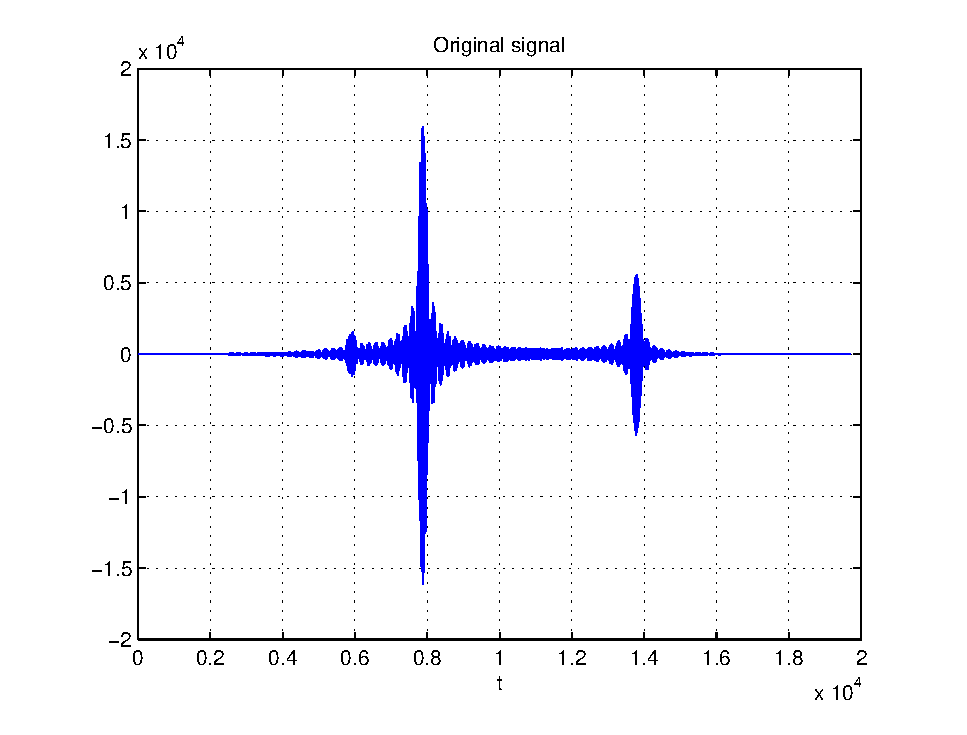
\includegraphics[height = 7.3 cm]{mmv_orig.eps}
\caption{An synthetic (time-domain) signal for the MMV model.}
\label{fig:mmv_orig}
\end{figure}

\begin{figure}[h]
\centering
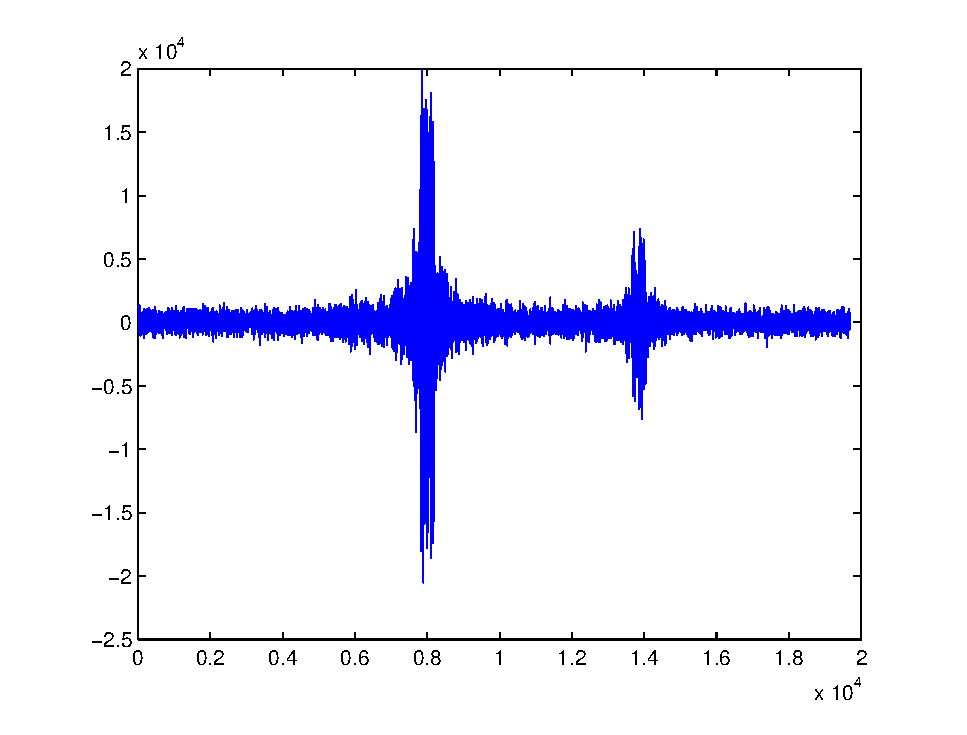
\includegraphics[height = 7.3 cm]{mmv_recon.eps}
\caption{Example reconstruction in the MMV model.}
\label{fig:mmv_recon}
\end{figure}


\section{Results} \label{sec:results}

The model described in section (\ref{sec:sensingmodel}), equation \eqref{system} was simulated, with a wideband signal of 201 channels and a network of 50 nodes (i.e. the signal will be sampled at a 1/4 of rate predicted by Nyquist theory). The mixing patterns were generated from iid Gaussian sources (i.e the matrix S had each entry drawn from an iid Gaussian source). Monte Carlo simulations were performed at SNR values ranging from 5 to 20, and the expected Mean Squared Error (MSE) of solutions of a centralised solver (spgl1) and a distributed solver (ADMM) were calculated over 10 simulations per SNR value. The results can be seen in fig (\ref{msevssnr1}). 

The MSE was calculated as follows:

\begin{equation}
\frac{\vectornorm{Z^k - Z*}}{\vectornorm{Z*}}
\end{equation}

where \(Z^k\) is the result of the algorithm at iteration \(k\), and \(Z^*\) is the optimal solution.

These results indicate that for both centralised and distributed solvers, adding noise to the system results in a degrading of performance. Interestingly note, that the distributed solver seems to (slightly) outperform the centralised solver at all SNRs. This is counter-intuitive, as it would be expected that centralised solvers knowing \textit{all} the available information would outperform distributed solutions. We conjecture that the updates described in section \eqref{sec:opt-on-graphs}, take into account differences in noise across the network. The distributed averaging steps, which form the new prior for each node, then penalise updates from relatively more noisy observations. This corroborates observations from \cite{bazerque2008}.

This observation is (partially) confirmed in figure (\ref{erroriterations}), which plots the progress of the centralised and distributed solvers (as a function of iterations) towards the optimum solution. The SNR is 0.5 (i.e the signal is twice as strong as the noise). Note that after around 300 iterations, the MSE of the distributed solver is consistently below that of the centralised solver.

\begin{figure}[h]
\centering
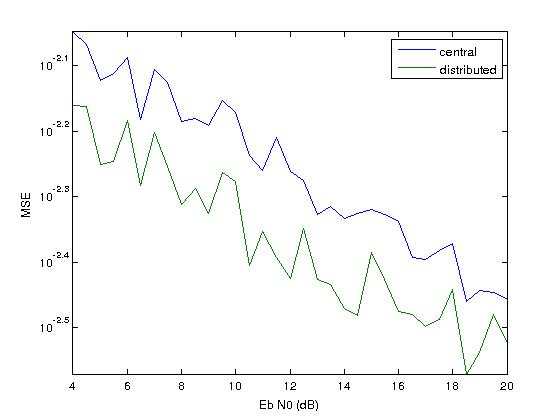
\includegraphics[height = 7.3 cm]{ebn0bbvsmse10ppnoH1logs.jpg}
\caption{Mse vs SNR for the sensing model, with AWGN only, showing the performance of distributed and centralised solvers}
\label{msevssnr0}
\end{figure}

\begin{figure}[h]
\centering
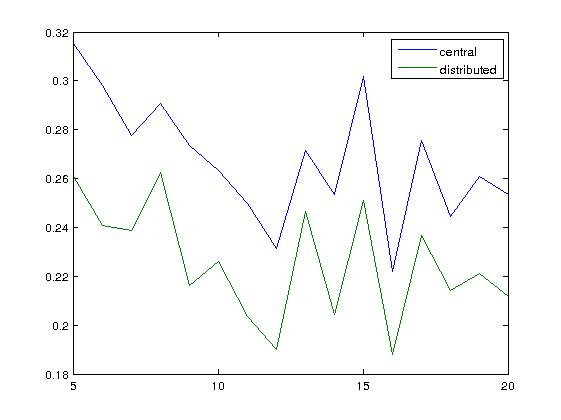
\includegraphics[height = 7.3 cm]{ebn0bbvsmse100ppwithH.jpg}
\caption{Mse vs SNR for the sensing model, showing the performance of distributed and centralised solvers}
\label{msevssnr1}
\end{figure}

\begin{figure}[h]
\centering
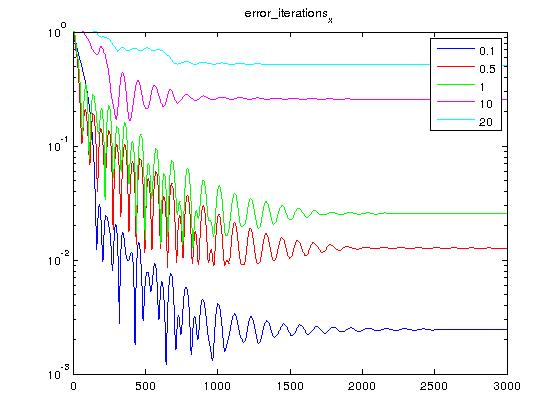
\includegraphics[height = 7.3 cm]{different_lambda.jpg}
\caption{The progress of the distributed solver as a function of the number of iterations, with different values of the regression parameter \(\lambda\)}
\label{fig:differentLambda}
\end{figure}

\begin{figure}[h]
\centering
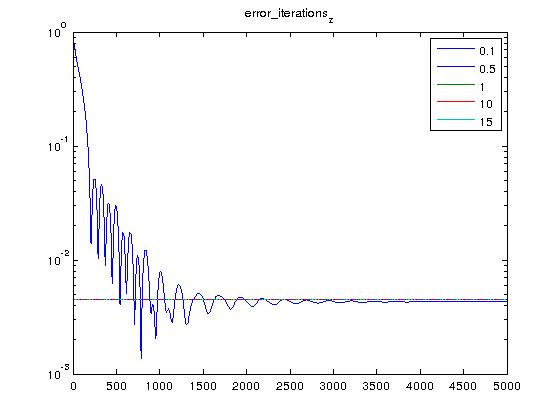
\includegraphics[height = 7.3 cm]{mse_iterations.jpg}
\caption{The progress of a distributed (blue) and a centralised (green) solver as a function of the number of iterations. The value of \(\lambda = 0.1\)}
\label{fig:erroriterations}
\end{figure}

\begin{figure}[h]
\centering
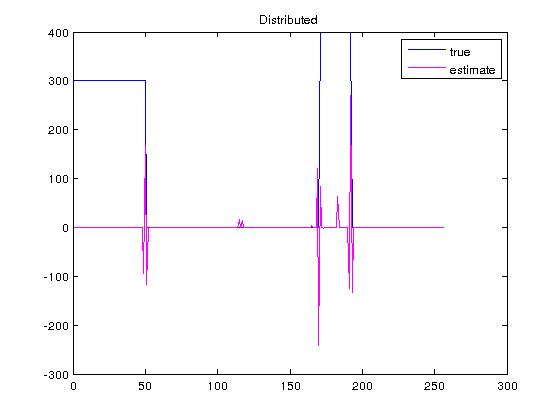
\includegraphics[height = 7.3 cm]{recon_spline.jpg}
\caption{The progress of a distributed (blue) and a centralised (green) solver as a function of the number of iterations. The value of \(\lambda = 0.1\)}
\label{fig:spline_recon}
\end{figure}

\begin{figure}[h]
\centering
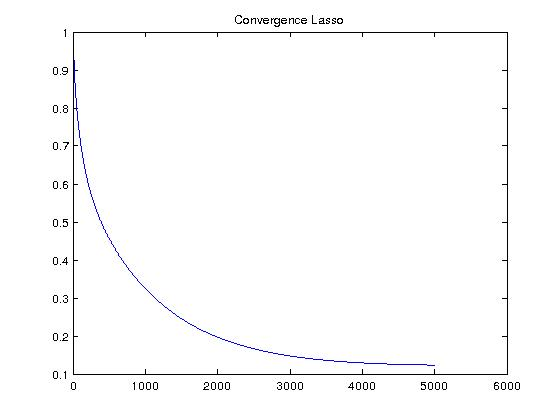
\includegraphics[height = 7.3 cm]{steps.jpg}
\caption{The progress of a distributed (blue) and a centralised (green) solver as a function of the number of iterations. The value of \(\lambda = 0.1\)}
\label{fig:steps_wavelets}
\end{figure}

\begin{figure}[h]
\centering
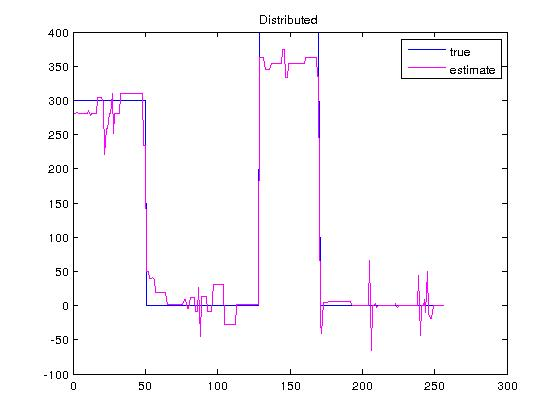
\includegraphics[height = 7.3 cm]{recon170815.jpg}
\caption{The progress of a distributed (blue) and a centralised (green) solver as a function of the number of iterations. The value of \(\lambda = 0.1\)}
\label{fig:wavelet_recon}
\end{figure}

\begin{figure}[h]
\centering
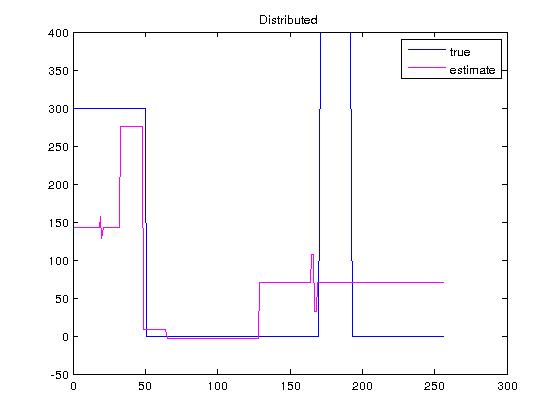
\includegraphics[height = 7.3 cm]{recon_new_bar.jpg}
\caption{The progress of a distributed (blue) and a centralised (green) solver as a function of the number of iterations. The value of \(\lambda = 0.1\)}
\label{fig:wavelet_recon_no_pwer_2}
\end{figure}

\begin{figure}[h]
\centering
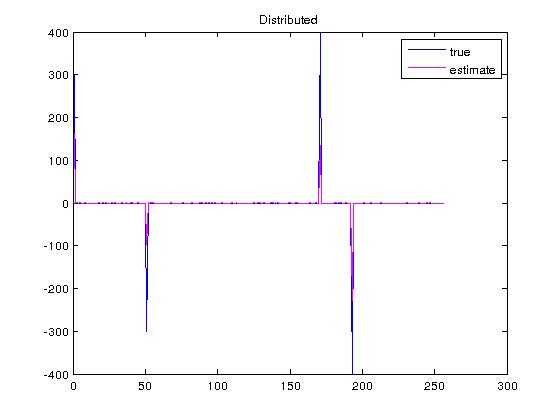
\includegraphics[height = 7.3 cm]{recon_difference.jpg}
\caption{The progress of a distributed (blue) and a centralised (green) solver as a function of the number of iterations. The value of \(\lambda = 0.1\)}
\label{fig:erroriterations}
\end{figure}

\begin{figure}[h]
\centering
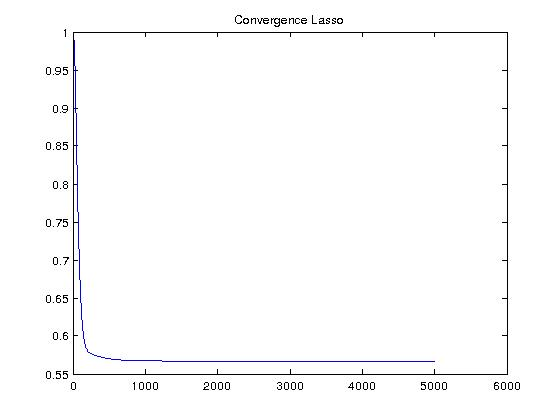
\includegraphics[height = 7.3 cm]{steps_difference.jpg}
\caption{The progress of a distributed (blue) and a centralised (green) solver as a function of the number of iterations. The value of \(\lambda = 0.1\)}
\label{fig:steps_difference}
\end{figure}

\begin{figure}[h]
\centering
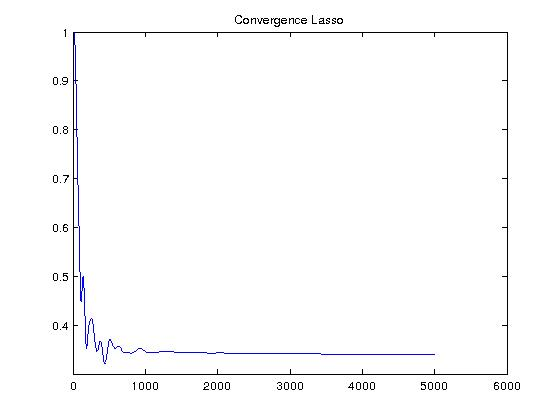
\includegraphics[height = 7.3 cm]{steps_splines.jpg}
\caption{The progress of a distributed (blue) and a centralised (green) solver as a function of the number of iterations. The value of \(\lambda = 0.1\)}
\label{fig:steps_splines}
\end{figure}

\begin{figure}[h]
\centering
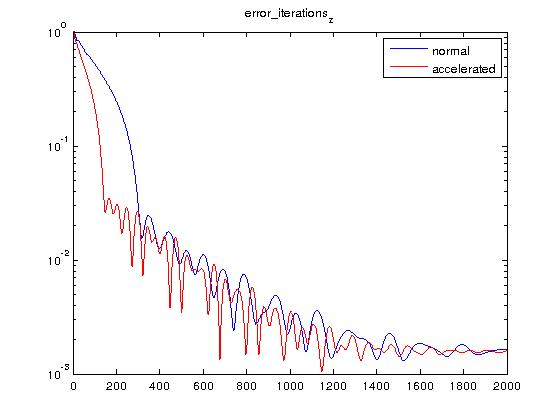
\includegraphics[height = 7.3 cm]{normalvsaccel.jpg}
\caption{The progress of a distributed (blue) and a centralised (green) solver as a function of the number of iterations. The value of \(\lambda = 0.1\)}
\label{fig:steps_splines}
\end{figure}

\section{Conclusions}
We have demonstrated an alternating direction algorithm for distributed optimisation with closed forms for the computation at each step, and discussed the statistical properties of the estimation. 

We have simulated the performance of this distributed algorithm for the distributed estimation of frequency spectra, in the presence of additive (white, Gaussian) and multiplicative (frequency flat) noise. We have shown that the algorithm is robust to a variety of SNRs and converges to the same solution as an equivalent centralised algorithm (in relative mean-squared-error).

We plan to work on larger, more detailed, models for the frequency spectra and to accelerate the convergence via Nesterov type methods to smooth the convergence of the distributed algorithm \cite{goldstein2014fast}. Specifically, we seek to dampen the ringing seen in Figure \ref{fig:erroriterations}
\include{cswireless_new_basis}
\documentclass[conference]{IEEEtran}
\bibliographystyle{IEEEtran}
\linespread{1.2}
\usepackage[margin = 1.25 in]{geometry}
\usepackage{wrapfig}
\usepackage{amsfonts}
\usepackage[utf8]{inputenc}
\usepackage[T1]{fontenc}
\usepackage{graphicx}
\usepackage[english]{babel}
\usepackage[algoruled]{algorithm2e}

\renewcommand{\theequation}{\thesection.arabic{equation}}

\renewcommand{\thefigure}{\thesection.\arabic{figure}}



\renewcommand{\vec}[1]{\mathbf{#1}}
\renewcommand{\theequation}{\thesubsection.\arabic{equation}}
\DeclareGraphicsExtensions{.pdf,.png,.jpg, .gif}

\usepackage{amsthm}

\usepackage[english]{babel}
\usepackage{mathtools}

%\usepackage[OT2,T1]{fontenc}
%\DeclareSymbolFont{cyrletters}{OT2}{wncyr}{m}{n}
%\DeclareMathSymbol{\sha}{\mathalpha}{cyrletters}{"58}

\DeclareFontFamily{U}{wncy}{}
\DeclareFontShape{U}{wncy}{m}{n}{<->wncyr10}{}
\DeclareSymbolFont{mcy}{U}{wncy}{m}{n}
\DeclareMathSymbol{\Sh}{\mathord}{mcy}{"58} 
\DeclareMathOperator*{\argmin}{arg\,min}

\newcounter{eqn}
\renewcommand*{\theeqn}{\alph{eqn})}
\newcommand{\num}{\refstepcounter{eqn}\text{\theeqn}\;}

\makeatother
\newcommand{\vectornorm}[1]{\left|\left|#1\right|\right|}
\newcommand*\conjugate[1]{\bar{#1}}

\newtheorem{thm}{Theorem}
\newtheorem{defn}{Definition}
 %\theoremstyle{plain}
  \newtheorem{theorem}{Theorem}[section]
  \newtheorem{corollary}[theorem]{Corollary}
  \newtheorem{proposition}[theorem]{Proposition}
  \newtheorem{lemma}[theorem]{Lemma}
\newtheorem{example}[theorem]{Example}
  \newtheorem{definition}[theorem]{Definition}
  \newtheorem{conj}[theorem]{Conjecture}
 \newtheorem{condition}{Condition}
 \newtheorem{remark}[theorem]{Remark}

\newcommand{\supp}{\operatorname{supp}} 
\newcommand{\vc}[1]{{\mathbf{ #1}}}
\newcommand{\tn}{\widetilde{\nabla}_{n} }
\newcommand{\Z}{{\mathbb{Z}}}
\newcommand{\re}{{\mathbb{R}}}
\newcommand{\II}{{\mathbb{I}}}
\newcommand{\ep}{{\mathbb{E}}}
\newcommand{\pr}{{\mathbb{P}}}
\newcommand{\FF}{{\mathcal{F}}}
\newcommand{\TT}{{\mathcal{T}}}
\newcommand{\phin}{\phig{n}}
\newcommand{\phig}[1]{\phi^{(#1)}}
\newcommand{\ol}[1]{\overline{#1}}
\newcommand{\eff}{{\rm eff}}
\newcommand{\suc}{{\rm suc}}
\newcommand{\tends}{\rightarrow \infty}
\newcommand{\setS}{{\mathcal{S}}}
\newcommand{\setP}{{\mathcal{P}}}
\newcommand{\setX}{{\mathcal{X}}}
\newcommand{\nec}{{\rm nec}}
\newcommand{\bd}{{\rm bd}}
\usepackage{algpseudocode}

\title{Distributed Compressive Spectrum Sensing}

\author{Thomas Kealy$^{1}$, Oliver Johnson$^{2}$ and Robert Piechocki$^{3}$% <-this % stops a space
\thanks{This work was supported by the Engineering and Physical Sciences Research Council [grant number {\tt EP/I028153/1}]; Ofcom; and the University of Bristol. The authors would particularly like to thank Gary Clemo of Ofcom for useful discussions.}%
\thanks{ $^{1}$Thomas Kealy is with CDT in Communications, MVB, School of Engineeering University of Bristol, UK
        {\tt\small tk12098@bristol.ac.uk}}%
\thanks{$^{2}$Oliver Johnson is with the Department of Mathematics, University Walk, Bristol, University of Bristol, UK.
        {\tt\small O.Johnson@bristol.ac.uk}}%
\thanks{$^{3}$Robert Piechocki is with the CSN Group, MVB, School of Engineering, University of Bristol, UK.
        {\tt\small r.j.piechocki@bristol.ac.uk}}%
}

\IEEEoverridecommandlockouts

\begin{document}

\maketitle

\begin{abstract}
\noindent Spectrum Sensing is a key technology for Cognitive Radio: the initial task of any cognitive device will be to accurately sense and classify spectral bands. The sampling rates required by many bands (for example TV Whitespaces) makes spectrum sensing costly with current technology. Currently many spectra are sparse and this sparsity can be exploited by using the modern paradigm of Compressive Sampling. A distributed network of sensors can further reduce the sensing load. Should these bands come into use, they will not remain sparse - this can be alleviated by requiring sparsity in the gradient of the spectrum. 

In this paper, we develop a model of the spectral gradient which allows reconstruction from Compressive measurements. Further, we develop a distributed ADMM algorithm for the LASSO with exact, closed form, expressions for the minima per iteration, reducing the computational cost of the algorithm. This allows us to perform spectral reconstruction which is blind to statistics such as the signal sparsity, using only simple statistical operations such as least squares and shrinkage. Numerical experiments show that the algorithm performs to within \(10^{-2}\) of an equivalent centralised algorithm. The algorithm displays the rapid convergence of ADMM, but with a substantially reduced computational burden.
\end{abstract}

\section{Introduction}

Spectrum Sensing is a key technology for Cognitive Radio. The initial task of any cognitive device, before any kind of dynamic spectrum management will be to accurately sense and classify spectral bands for availability. Dynamic management holds the promise of satisfying the almost ubiquitous growing demand for mobile and wireless data, with consumers demanding faster speeds and better quality connections in more places. However, there is constrained amount of frequencies over which to transmit this information; and demand for frequencies that provide sufficient bandwidth, good range and in-building penetration is high. Not all spectrum is used in all places and at all times, and judicious spectrum management, by developing approaches to use white spaces where they occur, would likely be beneficial.

Devices seeking to access white spaces need a robust mechanism for learning of the frequencies that can be used at a particular time and location. One approach is to refer to a database, which maps the location of white spaces based on knowledge of existing spectrum users. An alternative approach is for devices to detect white spaces by monitoring spectrum use. 

The advantages of spectrum monitoring \cite{akan2009cognitive} over persisting a database of space-frequency data are the ability of networks to make use of low-cost low-power devices, only capable of making local (as opposed to national) communications, keeping the cost of the network low and  opportunistic channel usage for bursty traffic, reducing channel collisions in dense networks. The main technical difficulty preventing spectrum sensing currently, are the high sampling rates required by wideband spectra such as TV white spaces (TVWS). However such spectra are typically sparse, in that transmissions use far fewer frequencies that the available bandwidth. 

Compressive Sensing (CS) \cite{Candes2006} has recently emerged as a new sampling paradigm, for acquiring sparse signals. Applying this to wireless communication, we are able to reconstruct sparse signals at sampling rates below what would be required by Nyquist theory, for example the works \cite{mishali2010theory}, and \cite{tropp2010beyond} detail how this sampling can be achieved. 

However, even with CS, spectrum sensing from a single machine will be costly as the proposed TVWS band will be over a large frequency range CS at a single sensor would still require high sampling rates \cite{Zhang2011b}. In this paper we propose a distributed model, which allows a sensing budget at each node far below what is required by centralised CS. The advantages of such a network are that is should be able to average out noise process across some geographic area by making distributed observations, and make use of cheaper sensors due to the lowered sensing budget required per node. 

We cannot always guarantee that the frequency spectrum will always be sparse: for example, should TVWS become widely utilised, the spectra will not be sparse. However, even for highly occupied spectra, the gradient of the spectrum will be sparse. This has previously been exploited by \cite{tian2006wavelet}. 

Reconstructing the spectrum from compressive measurements could take place at a fusion centre, but such communications are expensive. It is more efficient therefore to design distributed algorithms where CRs communicate with their neighbours to reach consensus on the reconstruction, given each nodes' private data. However, regularising the reconstruction process would require global co-ordination if Total Variation (the \(l_1\) norm of the gradient of the signal) regularisation was chosen, as.

In this paper we propose a different model for sensing the gradient of the frequency spectrum to \cite{tian2006wavelet} - a model which doesn't require Total Variation regularisation of the objective function. 

We also propose a decentralised algorithm to solve the LASSO by consensus optimisation. This allows us to design an algorithm which requires no global co-ordination whilst reconstructing the gradient of the spectrum. We choose a convex approach, as convex algorithms require no knowledge of the signal statistics (such as sparsity), and are guaranteed to converge. We are able to find exact, closed form, expressions for the Distributed Lasso, reducing the computational load per iteration whilst obviating the need to approximate the objective function \cite{ling2014dlm}.

The structure of the paper is as follows: in section \ref{sec:sensingmodel} we introduce the sensing model, in section \ref{sec:opt-on-graphs} we describe the distributed reconstruction algorithm \cite{mota2013d}, and finally in section \ref{sec:results} we show some results of the reconstruction quality of this model. 

\section{Signal Model}

Not all signals are sparse in an orthogonal basis: for example, many images are sparse in an over-complete dictionary (set of bases). In particular, frequency spectra for TVWS may no longer be sparse once opportunistic radios begin operating in these frequency bands. 

Instead we aim to reconstruct the gradient of the spectrum, as we assume that transitions are constant within a band. Consider the basis defined by the function:

\begin{equation}
l_i\left(x\right) =
\begin{cases}
1 & \text{if } x \leq i \\
0 & \text{ otherwise } 
\end{cases}
\label{basis}
\end{equation}

That is, \(l_i\) is a left-hand step function. 

The basis (\ref{basis}) can be expressed as a matrix in \(\re^{n \times n}\) as:

\begin{equation}
L = \begin{pmatrix}
 1 & 0 & 0 & 0  & 0 \ldots 0 \\
  1 & 1 & 0 & 0  & 0 \ldots 0\\
     1 & 1 & 1 & 0  & 0 \ldots0  \\
    \ldots  \\
     1 & 1 & 1 & 1  & 1 \ldots 1 
\end{pmatrix}
\end{equation}

By direct computation, this inverse of \(L\) is:

\begin{equation}
D = \begin{pmatrix}
 1 & 0 & 0 & 0  & 0 \ldots 0 \\
  -1 & 1 & 0 & 0  & 0 \ldots 0\\
     0 & -1 & 0 & 0  & 0 \ldots0  \\
    \ldots  \\
     0 & 0 & 0 & 0  \ldots -1 & 1
\end{pmatrix}
\end{equation}

We model our PSD signal \(g\) as a linear combination of the basis functions (\ref{basis}):

\begin{equation}
g\left(x\right) = \sum_i a_i l_i\left(x\right) = L^Ta
\label{basis-expansion}
\end{equation}

where \(a = (a_1, \ldots, a_n\) are the coefficients in this basis expansion, and \(l_i\) are the rows of \(L\). Note that as defined, \(g\) is a column vector.

\begin{proposition}
\begin{equation}
D^Tg = a
\end{equation}
\label{def:a}
\end{proposition}
\begin{proof}

\begin{align}
D^Tg &= D^T L^T a \\
&= \left(LD\right)^Ta \\
&= a
\end{align}

as \(LD = I\).

\end{proof}

\section{Sensing Model}\label{sec:sensingmodel}

We consider a radio environment with a single primary user (PU) and a network of \(J\) nodes collaboratively trying to sense and reconstruct the PU signal in a fully distributed manner by local communication and regularisation only.

We try to sense and reconstruct a wideband signal, using a network of \(J\) (= 50) nodes placed uniformly at random within the square \(  \left[0,1\right]\times \left[0,1\right] \). 

We consider the frequency domain measurements, formed by each node mixing the signal with a random Gaussian signal \(A_j \in \re^n\). The measurements taken at node \(j\) are:

\begin{equation}
y_j = A_jH_jg + w_j
\label{dist_system}
\end{equation}

where \(H_j \in \re\) is the scalar channel gain, and \(w_j \sim \mathcal{N}(0,\sigma^2_n) \in \re \) is additive white Gaussian noise. 

For the purposes of comparison in section (\ref{sec:results}), this corresponds to the concatenated system:

\begin{equation}
y = AHg + w
\label{system}
\end{equation}

where \(H \in \re^{n \times n}\) is a block diagonal matrix of channel gains.

The system  \ref{system} can then be solved (in the sense of finding the sparse vector \(a\) (\ref{basis}) by convex optimisation via minimising the objective function:

\begin{equation}
\hat{a} = \argmin_{a} \frac{1}{2}\|AHL^{T}a-y\|_2^2 + \lambda \|a\|_1
\label{opt}
\end{equation}

where \(\lambda\) is a parameter chosen to promote sparsity. Larger \(\lambda\) means sparser \(a\).

\section{Constrained Optimisation on Graphs}\label{sec:opt-on-graphs}

We model the network of sensors as an undirected graph \(G = \left(V,E\right)\), where \(V = \{1 \ldots J\}\) is the set of vertices, and \(E = V \times V\) is the set of edges. An edge between nodes \(i\) and \(j\) implies that the two sensors can communicate. The set of nodes that node \(i\) can communicate with is written \(\mathcal{N}_i\) and the degree of node \(i\) is \(D_i = |\mathcal{N}_i|\). 

We assume that a proper colouring of the graph is available: that is, each node is assigned a number from a set \(C = \{1 \ldots c \} \), and no node shares a colour with any neighbour. This is so that nodes may communicate in colour order, as opposed to communicating individually thus reducing the total number of communication rounds required. 

Individually nodes make the following measurements (as discussed in section \ref{sec:sensingmodel}):

\begin{equation}
\vec{y}_j = \vec{M}_j\vec{x} + \vec{n}_j
\end{equation}

where \(\vec{M}_j = \left(\vec{AHL^T}\right)_j \) is the \(p^{th} \) row of the sensing matrix from \eqref{system}.

To find the \(\vec{x}\) we are seeking (the solution to \eqref{opt}, to each node we give a copy of \(\vec{x}\), \(\vec{x}_j \in \re^n\), and we constrain the copies to be identical across all edges in the network. To separate the minimisation of the \(\ell_2\) and \(\ell_1\) norms, we also introduce a dummy variable \(\vec{z}_j \in \re^n\) to each node. Each node, thus has a separate optimisation to solve, subject to the constraint that it is consistent with its neighbours.

We write the global optimisation variable as \(\bar{x}\), which collects together \(C\) copies of a \(n\times 1\) vector \(\vec{x}\):

\begin{defn}
We define vectors \(x_c\) which represent the subset of nodes with colour \(c\), where \(c = 1,\ldots , C\), and write the vector of length \(nJ\):
\begin{equation}
\bar{x} = \sum_{c=1}^C w_c \otimes x_c = \left[x_{c(1)}^T, \ldots	, x_{c(J)}^T\right]^T
\label{barxc}
\end{equation}
where \(w_{c(i)} = \mathbb{I}(c(i) = c)\), \(\mathbb{I}\) is the indicator function, and we have written \(c(i)\) for the colour of the \(i\)th node.
\end{defn}

The problem then is to solve:

\begin{align}
\argmin_{\bar{x}} \sum_{c=1}^C \sum_{j \in c} \|M_jx_j - y_j\|_2^2 + \frac{\lambda}{J}\|z\|_1 \nonumber \\ 
\text{ and } x_i = x_j \text{ if } \{i,j\} \in E \nonumber \\
\text{ and } x_i - z_i = \text{ } \forall i \in \{1, \ldots, C\}
\label{constrainedbp}
\end{align}

That is, at each node we minimise a Lasso functional constrained to be consistent across edges, but that is separable in the \(\ell_2\) and \(\ell_1\) norms.

The first set of constraints (edge-agreement) can be written more compactly by introducing the node-arc incidence matrix B: a \(V\) by \(E\) matrix where each column is associated with an edge \(\left(i,j\right) \in E\) and has \(1\) and \(-1\) in the \(ith\) and \(jth\) entry respectively. We require that \( Bx_j = 0 \) for all nodes \(j = 1, \ldots,  J\). The global constraint is simply \( (B \otimes I_n)\bar{x} = 0\), and using definition \eqref{barxc} the constraint \(x_i = x_j \text{ if } \{i,j\} \in E \) can now be written:

\begin{equation}
\sum_{c=1}^C\left(B_c^T \otimes I_n\right)\bar{x}_c = 0
\label{compact-constraints}
\end{equation}

note that \(\left(B^T\otimes I_n \right) \in \re^{nE \times nJ}\).

 Together \eqref{barxc} and \eqref{compact-constraints}, suggests that the problem \eqref{constrainedbp} can be re-written as:

\begin{align}
\argmin_{\bar{x}} \sum_{c=1}^C \sum_{j \in C_c} \|M_jx_j - y_j\|_2^2 + \beta\|z_j\|_1
\nonumber \\
\text{ s.t. } \sum_{c=1}^C\left(B_c^T \otimes I_n\right)\bar{x}_c = 0 \nonumber \\
\text{ and } \bar{x}_c - \bar{z}_c = 0
\label{constrainedbp1}
\end{align}

where \(\beta = \frac{\lambda}{J}\).

The global Augmented Lagrangian \cite{Boyd2010a}
 for the problem \eqref{constrainedbp1} can be written down as:

\begin{align}
L_\rho = \sum_{c=1}^C  \biggl( \sum_{j \in c} & \|M_jx_j - y_j\|_2^2 + \beta\|z_j\|_1  + \nonumber \\ & + \theta^T\left(\bar{x}_j - \bar{z}_j\right)  +  \frac{\rho}{2}\vectornorm{\bar{x}_j-\bar{z}_j}_2^2 \biggr) + \nonumber \\  & + \eta^T\left(B_c^T \otimes I_n\right)\bar{x}_c + \frac{\rho}{2}\vectornorm{\sum_{c=1}^C\left(B_c^T \otimes I_n\right)\bar{x}_c}_2^2
\label{aug-lagrange}
\end{align}

This is, superficially, similar to the Augmented Lagrangian for the Lasso problem \cite{Boyd2010a}[Section 6.4]. That is, the terms indexed by \(j\) are a straightforward Lasso problem, constrained by edge-wise variables (indexed by \(c\)) forcing consistency across the network. However, the problem (as currently written) is not separable across the edges of the network as the final and penultimate term represent the constraint that the nodes agree on their estimates across edges. 

To make it possible that \ref{aug-lagrange} can be posed  as a constrained optimisation problem at each node, we introduce the following variable:

\begin{defn}[Edge-equality vector]
\begin{align*}
u &:= \left(B^T \otimes I_n\right)\bar{x} \\
& = \left(B^T \otimes I_n\right)\sum_{c=1}^C w_c \otimes x_c \\
& = \sum	_{c=1}^C B_c^T\otimes x_c
\end{align*}
where we have used the definition \eqref{barxc} in the second line, the property of Kronecker products \((A\otimes C)(B \otimes D) = (AB \otimes CD)\) between the second and third lines, and we write \(B_c = w_c^TB\).
\end{defn}

The terms \(\|\sum_{c=1}^C\left(B_c^T \otimes I_n\right)\bar{x}_c\|^2\) and \( \eta^T\left(B_c^T \otimes I_n\right)\bar{x}_c \) of \eqref{aug-lagrange}, can be decomposed across edges, using the following lemma:

\begin{lemma}[Edge Decomposition]
\begin{equation}
\vectornorm{\sum_{c=1}^C\left(B_c^T \otimes I_n\right)\bar{x}_c}^2 = \sum_{j \in C_c}\left( D_j\vectornorm{x_j}_2^2 - \sum_{k \in \mathcal{N}_j} x_j^Tx^k\right)
\end{equation}

and

\begin{equation}
\eta^T\sum_{c=1}^C\left(B_c^T \otimes I_n\right)\bar{x}_1 = \sum_{l\in C_c} \sum_{m\in \mathcal{N}_l}\mathrm{sign}\left(m-l\right)\eta_{ml}^T x_l
\end{equation}

where \(\eta\) is decomposed edge-wise: \(\eta = \left(\ldots, \eta_{ij},\ldots\right)\), such that \(\eta_{i,j} = \eta_{j,i}\), and is associated with the constraint \(x_i = x_j\).


\begin{proof}
For the first part, note that 
\begin{align*}
u^Tu &= \vectornorm{\sum_{c=1}^C\left(B_c^T \otimes I_n\right)\bar{x}_c}^2 
\\ &=\sum	_{c_1=1}^C \sum	_{c_2=1}^C  \left(B_{c_1} \otimes x_{c_1}^T\right) \left(B_{c_2}^T \otimes x_c\right) \\
&= \sum_{c_1, c_2} B_{c_1}B_{c_2}^T \otimes x_{c_1}^Tx_{c_2}
\end{align*}

\(BB^T\) is a \(J \times J\) matrix, with the degree of the nodes on the main diagonal and \(-1\) in position \(\left(i,j\right)\) if nodes \(i\) and \(j\) are neighbours (i.e \(BB^T\) is the graph Laplacian). Hence, since we can write \(B_{c_1}B_{c_2}^T = w_{c_1}^TBB^Tw_{c_2}\), the trace of \(B_{c_1}B_{c_1}^T\) is simply the sum of the degrees of nodes with colour 1. Similar reasoning applies to all other colours.

For \(c_1 \neq c_2\),  \(B_{c_1}B_{c_2}^T\) corresponds to an off diagonal block of the graph Laplacian, and so counts how many neighbours each node with colour 1 has.

For the second part note that \(\eta \in \re^{nE}\) and can be written:

\begin{equation}
\eta = \sum_{c=1}^C w_c \otimes \eta_c
\end{equation}
where \(\eta_c\) is the vector of Lagrange multipliers associated across edges from colour \(c\). Now

\begin{align*}
\eta^Tu = \sum_{c_1=1}^C\sum_{c_2=1}^C w^T_{c_1}Bw_{c_2} \otimes \eta_{c_1}^Tx_{c_2}
\end{align*}
where we have repeated the reasoning from the previous part: using the properties of Kronecker products, and the definition of \(B_c\). For \(c_1=c_2\), \(\eta^Tu\) is zero, as there are no edges between nodes of the same colour by definition. For \(c_1\neq c_2\), \(\eta^Tu\) counts the edges from \(c_1\) to \(c_2\), with the consideration that the edges from \(c_2\) to \(c_1\) are counted with opposite parity. I.e. for a node \(l\) with colour \(C\), \(w_{c_1}^TB_{c_2}\) counts the edges to the neighbours of node \(l\), and the edges from the neighbours of node \(l\) to node \(l\) with opposite parity - \(\mathrm \sum_{l\in C_c} \sum_{m \in N_l} \mathrm{sign}(m-l)\).
\end{proof}
\end{lemma}

\begin{figure}
\begin{algorithmic}[1]
\Procedure{DADMM}{$y_j,M_j,\varepsilon$}
\State $x^0 = 0$, $z^0 = 0$, $\theta^0 = 0$, $\eta^0 = 0$, \\  $Q =  \left(M_j^TM_j + (\rho D_J + 1) I\right)^{-1}$, $w_j = M_j^Ty_j $
\While{$\vectornorm{z^{k+1} - z^{k}} \leq \varepsilon$}
\For{$c = 1, \ldots, C}$
\State $x^{k+1} \gets Q\left(w_j+  z^k - \theta^{kT} -\nu^{kT}\right)$  
\State  $z^{k+1} \gets S_{\beta/\rho}\left(x_j^{k+1} \right) $  
\State $\theta^{k+1}\gets \theta_j^{k} + \rho \left(x^{k+1}-z^{k+1}\right)$  
\EndFor
\\Each node transmits $x^{k+1}$ in $\mathcal{N}_j$ and calculates
  \State $\nu_j^{k+1} \gets \nu_j^k + \rho\left(\sum_{m \in N_j} z_m^k - z_j^k\right)$
\EndWhile
\State \textbf{return} $z^{k+1}$
\EndProcedure
\end{algorithmic}
\caption{The algorithm at Node \(j\)}\label{DADMM}
\end{figure}

Adding together this with the lemma, lets us write \eqref{aug-lagrange} as:

\begin{align}
L_\rho = \sum_{c=1}^C \biggl( \sum_{j \in C_c} \|M_jx_j - y_j\|_2^2 + \beta\|z_j\|_1 + \nu^Tx_j \nonumber \\
 + \theta\left(x_j - z_j\right) + \frac{\rho}{2}D_i\vectornorm{x_j}^2 + \frac{\rho }{2}\vectornorm{x_j-z_j}^2 \biggr)
\label{generic-iterations}
\end{align}

where we have defined:

\begin{equation}
\nu_i = \left(\sum_{k \in \mathcal{N}_i} sign\left(k-i\right)\eta_{\{i,k\}} - \rho x_k \right)
\end{equation}

which is a rescaled version of the Lagrange multiplier, \(\eta\), which respects the graph structure. 

Then by differentiating \eqref{generic-iterations} with respect to \(x_j\) and \(z_j\) we  can find closed forms for the updates as:

\begin{align}
x_j^{k+1} &:= \left(M_j^TM_j + (\rho D_J + 1) I\right)^{-1}\left(M_j^Ty_j +  z^k -\theta^{kT} - \nu^{kT}\right)\\
z_j^{k+1} &:= S_{\beta/\rho}\left(x_j^{k+1} \right)
 \\
\theta_j^{k+1} &:= \theta_j^{k} + \rho \left(x^{k+1}-z^{k+1}\right) \\
\nu_j^{k+1} &:= \nu_j^k + \rho\left(\sum_{m \in \mathcal{N}_j} z_m^k - z_j^k\right)
\label{dadmm_algo_lasso}
\end{align}

Where we have defined

\begin{defn}[Soft-thresholding]
\begin{equation}
S_{\tau}\left( y \right) := \mathrm{sign}(y)\mathrm{max}(y-|\tau|, 0)
\end{equation}
\end{defn}

\begin{remark}
This algorithm can be thought of as a distributed EM algorithm with memory: each node places a Gaussian prior with variance proportional to its degree on its private data, and solves a posterior least-squares problem. Each node then soft thresholds and then exchanges the result of this computation with its one-hop neighbours.
 
This explains the inclusion of an extra Lagrange multiplier: the multiplier \(\theta\) controls how far each node moves from its previous estimate in each iteration, whilst the multiplier \(\eta\) enforces consistency between nodes by integrating past disagreements between neighbouring nodes. Note that there is no communication of data between the nodes - only the result the computation in each round.
\end{remark}

\section{Results} \label{sec:results}

The model described in section \eqref{sec:sensingmodel}, equation \eqref{system} was simulated. The signal \(g \in \re^{300} \) was composed of 3 rectangular pulses, mimicking primary user signals in TVWS, as shown in figure \eqref{different_sigs} (a). The signal was put through a Rayleigh channel, before being sensed by the nodes. The network was generated as a random geometric graph in \([0,1] \times [0,1]\), with 50 nodes. If the network wasn't connected, it was redrawn. 200 mixing patters were drawn i.i.d from a \(\mathcal{N}\left(0, \sigma^2 I_{300} \right) \) distribution, with \(\sigma^2 = 1/200\), to from the matrix \(A\in  \re^{200 \times 300}\).

Monte Carlo simulations were performed at 18 \(\sigma^2_n\) values ranging from 1 to 10 and the expected Mean Squared Error (MSE) of solutions of a centralised ADMM solver and a our distributed solver were calculated over 500 repetitions with 1200 iterations (\(k\)) per repetition.

The MSE was calculated as follows:

\begin{equation}
\frac{\vectornorm{L^tz^k - g^*}}{\vectornorm{g^*}}
\end{equation}

where \(z^k\) is the result of the algorithm at iteration \(k\), and \(g^*\) is the optimal solution.

The SNR for each repetition was calculated as

\begin{equation}
\frac{\vectornorm{g^*}}{\vectornorm{w}}
\end{equation}

and averaged over the 500 repetitions. The results are shown in figure \eqref{msevssnr0}. Following \cite{chen1998atomic}, for each repetition we chose 

\begin{equation}
\lambda = \sqrt{2\sigma^2_n\log{n}}
\end{equation}

The error bars indicate the empirical variance across the 500 repetitions.

These results indicate that for both the centralised and distributed solvers, their performance degrades as the noise power increases in a roughly log-linear fashion. The performance of the distributed algorithm is consistently worse than the centralised version, this contrasts with results from \cite{bazerque2008}; this is due to the differing sparsity models: \cite{bazerque2008} use a joint space and frequency model for the sparsity, and as such observe an spatial averaging out of noise when using a distributed solver. The performance of DADMM is within the error bars of the centralised version at low SNR, and gap in performance between the two versions is no more than \(10^{-2}\). Even at relatively lower SNRs both solvers reach a solution within \(10^{-1}\) of the optimal (as measured by normalised MSE), which will be adequate for the task of spectrum sensing. For example the reconstructions in figures \eqref{different_sigs} (c) and (d) show realisations of the reconstruction from DADMM with \(\sigma^2_n = 5\) and \(\sigma^2_n = 20\) respectively. It is still possible to distinguish the occupied bands from unoccupied frequencies for both reconstructi	ons.

The distributed algorithm has consistently larger variance, than the centralised solver at all SNRs. This is due to individual nodes only having access to a subset of the data to perform calculations on: the variance will be proportional to the square-root of number of data samples at each node, which are fewer than the total number of samples available to the centralised solver. 

In figure \eqref{fig:differentLambda}, we plot the progress of DADMM along the solution path for a variety of regularisation parameters \(\lambda\). The y-axis is the relative (unormalised) MSE between the optimal solution and the current iteration, and the x-axis is the iteration number. We note that for a fixed \(\lambda\) there is a single unique optimal solution, which DADMM converges to (in the sense of stationary error between consecutive iterations). This solution may not be attained in the allotted number of iterations, as the rate of convergence is determined by \(\lambda\), \(\rho\) and the eigenvalues of the Laplacian of \(G\). The paper \cite{DADMMconvergence}, proves linear convergence for DADMM, with explicit expressions for the rate. In particular the rate convergence of DADMM is affected by the choice of \(\lambda\): smaller \(\lambda\) corresponds to slower convergence - this is intuitive as solutions with fewer non-zero components should require fewer iterations to fully specify. Notice that for some \(\lambda\)s the solution path exhibits phenomenological  behaviour similar to damped oscillations: this phenomena has been explored in \cite{nishihara2015general} and \cite{su2014differential}.  

\begin{figure}[h]
\centering
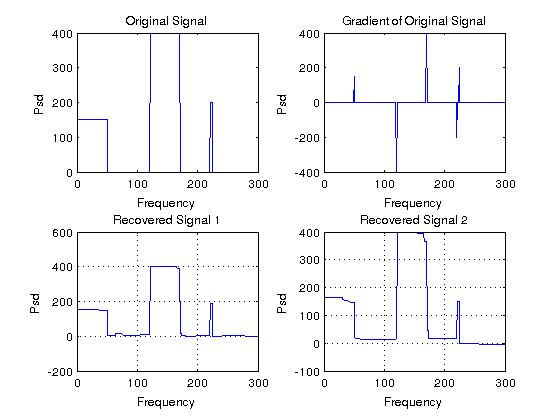
\includegraphics[height = 7.3 cm]{signal_and_recovery.jpg}
\caption{Left to right: (a) The original signal. (b) The gradient \eqref{def:a} of the original signal. (c) Recovery using DADMM, 1000 iterations, \(\sigma^2_n = 5\). (d) Recovery using DADMM, 1000 iterations, \(\sigma^2_n = 20\)  }
\label{different_sigs}
\end{figure}

\begin{figure}[h]
\centering
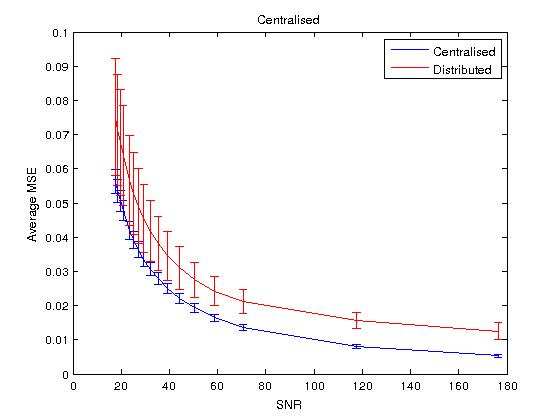
\includegraphics[height = 7.3 cm]{Cent_Vs_Distrib_snr.jpg}
\caption{MSE vs SNR for the sensing model showing the performance of distributed and centralised solvers. The performance of DADMM is consistently within \(10^{-2}\) of ADMM, and within the error bars of ADMM at low SNRs. The variance of estimates produced by DADMM is larger than ADMM, due to nodes performing computations on a subset of data. Both estimates are consistently within \(10^{-1}\) of the optimal solution, which is sufficient to classify occupied bands.} 
\label{msevssnr0}
\end{figure}

\begin{figure}[h]
\centering
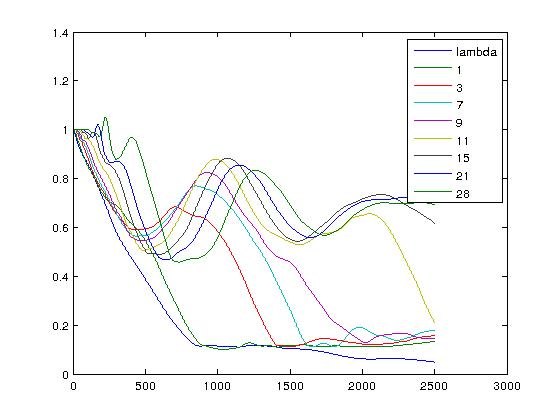
\includegraphics[height = 7.3 cm]{continuations_errors.jpg}
\caption{The progress of the distributed solver as a function of the number of iterations, with different values of the regression parameter \( \lambda \). For a fixed \( \lambda \) there is a single unique optimal solution, with higher \( \lambda \) favouring sparser solutions. The convergence of DADMM is slowed by smaller \( \lambda \). This is intuitive: solutions with fewer non-zero components should be identified in fewer iterations.}
\label{fig:differentLambda}
\end{figure}

\section{Conclusions}
We have demonstrated an alternating direction algorithm for distributed optimisation with exact (as opposed to linear or quadratic approximations to the objective as in \cite{mokhtari2015dqm} and \cite{ling2014dlm}) closed form expressions for the computation at each iteration, and discussed the statistical properties of the estimation. 

We have simulated the performance of this distributed algorithm for the distributed estimation of frequency spectra, in the presence of additive (white, Gaussian) and multiplicative noise. We have shown that the algorithm is robust to a variety of SNRs and converges to a similar solution as an equivalent centralised algorithm (in relative mean-squared-error).

We plan to work on larger, more detailed, models for the frequency spectra, to extend our regression framework to solve the MMV problem, to accelerate the convergence via Nesterov type methods to smooth the convergence of the distributed algorithm \cite{goldstein2014fast}, and to incorporate spatial variation into our model to further promote sparsity. We also plan to automate the choice of \(\lambda\) via continuation methods, and study how the choice of \(\lambda\) and \(\rho\) affect the rate of convergence. 

\bibliography{cswireless3}

\end{document}
\documentclass{article}
\bibliographystyle{plain}
\linespread{1.2}
\usepackage[margin = 1.25 in]{geometry}
\usepackage{wrapfig}
\usepackage{amsfonts}
\usepackage[utf8]{inputenc}
\usepackage[T1]{fontenc}
\usepackage{graphicx}
\usepackage[english]{babel}
\usepackage[algoruled]{algorithm2e}

\renewcommand{\theequation}{\thesection.arabic{equation}}

\renewcommand{\thefigure}{\thesection.\arabic{figure}}



\renewcommand{\vec}[1]{\mathbf{#1}}
\renewcommand{\theequation}{\thesubsection.\arabic{equation}}
\DeclareGraphicsExtensions{.pdf,.png,.jpg, .gif}

\usepackage{amsthm}

\usepackage[english]{babel}
\usepackage{mathtools}

%\usepackage[OT2,T1]{fontenc}
%\DeclareSymbolFont{cyrletters}{OT2}{wncyr}{m}{n}
%\DeclareMathSymbol{\sha}{\mathalpha}{cyrletters}{"58}

\DeclareFontFamily{U}{wncy}{}
\DeclareFontShape{U}{wncy}{m}{n}{<->wncyr10}{}
\DeclareSymbolFont{mcy}{U}{wncy}{m}{n}
\DeclareMathSymbol{\Sh}{\mathord}{mcy}{"58} 
\DeclareMathOperator*{\argmin}{arg\,min}

\newcounter{eqn}
\renewcommand*{\theeqn}{\alph{eqn})}
\newcommand{\num}{\refstepcounter{eqn}\text{\theeqn}\;}

\makeatother
\newcommand{\vectornorm}[1]{\left|\left|#1\right|\right|}
\newcommand*\conjugate[1]{\bar{#1}}

\newtheorem{thm}{Theorem}
\newtheorem{defn}{Definition}
 %\theoremstyle{plain}
  \newtheorem{theorem}{Theorem}[section]
  \newtheorem{corollary}[theorem]{Corollary}
  \newtheorem{proposition}[theorem]{Proposition}
  \newtheorem{lemma}[theorem]{Lemma}
\newtheorem{example}[theorem]{Example}
  \newtheorem{definition}[theorem]{Definition}
  \newtheorem{conj}[theorem]{Conjecture}
 \newtheorem{condition}{Condition}
 \newtheorem{remark}[theorem]{Remark}

\newcommand{\supp}{\operatorname{supp}} 
\newcommand{\vc}[1]{{\mathbf{ #1}}}
\newcommand{\tn}{\widetilde{\nabla}_{n} }
\newcommand{\Z}{{\mathbb{Z}}}
\newcommand{\re}{{\mathbb{R}}}
\newcommand{\II}{{\mathbb{I}}}
\newcommand{\ep}{{\mathbb{E}}}
\newcommand{\pr}{{\mathbb{P}}}
\newcommand{\FF}{{\mathcal{F}}}
\newcommand{\TT}{{\mathcal{T}}}
\newcommand{\phin}{\phig{n}}
\newcommand{\phig}[1]{\phi^{(#1)}}
\newcommand{\ol}[1]{\overline{#1}}
\newcommand{\eff}{{\rm eff}}
\newcommand{\suc}{{\rm suc}}
\newcommand{\tends}{\rightarrow \infty}
\newcommand{\setS}{{\mathcal{S}}}
\newcommand{\setP}{{\mathcal{P}}}
\newcommand{\setX}{{\mathcal{X}}}
\newcommand{\nec}{{\rm nec}}
\newcommand{\bd}{{\rm bd}}

\DeclareUnicodeCharacter{00A0}{~}

\title{Compressive Filtering}
\author{Tom Kealy}

\begin{document}
\maketitle

\section{Classical Filtering and Compressive Sensing}

Compressive Sensing has established that non-uniform sampling with random waveforms can be used to capture low-complexity signals, at rates far below those specified by Nyquist. The work of Candes and Tao \cite{Candes2006} and Donoho \cite{donoho2006compressed} has established that this sensing framework is universal: the sensing mechanism and reconstruction algorithms are insensitive as to whether the signal is an image, a song, or frequency spectra as long as it is sparse. The computational effort in these systems is backloaded to the reconstruction algorithm, which can have considerable computational complexity. This is in contrast to traditional sampling \cite{unser}, where the processing required to obtain the digital samples is the difficult part. Classical reconstruction is simply interpolation through an appropriate filter.

There are some technical specifications that on the compressive sensing mechanism which means that it can achieve this dimensionality reduction. Firstly the sensing waveforms must be incoherent with the signals being sensed \cite{candes2008introduction}. This is a statement similar to the \(T_s\)-spaced delta function requirement from classical sensing: we need to sample the signal in a domain where its information is spread out. As a signal cannot be sparse in two bases simultaneously, we can exploit the uncertainty relation between the bases to sample the signal efficiently. The other requirement on the sensing waveforms is that they are orthogonal, and change the norm of the signal by very little. In particular, they must not send the signal to \(0\), or recovery would be impossible.

The structure of this document is as follows: sections \eqref{sec:prelims}, is a literature review of relevant material from compressed sensing, Wishart matrices, and maximum likelihood estimation of uncompressed signals in noise. Section \eqref{sec:estimation} gives an overview of the problem of estimating a signal from a known set of basis functions. 

\subsection{Classical Sampling}

Classically, for perfect signal reconstruction, we must sample a signal such that the sampling rate must be at least twice the maximum frequency in the bandlimited signal \cite{unser}. The continuous time signal can then be recovered using an appropriate reconstruction filter (e.g. a sinc filter). For example, we can represent a sampled continuous signal as a multiplication of the signal with a train of Dirac delta functions at multiples of the sampling period T.
%
\begin{equation}
x\left(nT\right) = \Sh\left(t-nT\right)x\left(t\right)
\end{equation}
%
where
%
\begin{equation}
\Sh\left(t-nT\right) = \sum_{k=-\infty}^{\infty} \delta\left(t - kT\right)
\end{equation}

Working the frequency domain, this multiplication becomes convolution (which is equivalent to shifting):

\begin{equation}
\hat{X}_{s}\left(f\right) = \sum_{k=-\infty}^\infty x\left(t - kT\right)
\end{equation}

Thus if the spectrum of the frequency is supported on the interval \(\left(-B, B\right)\) then sampling at intervals \(\frac{1}{2B}\) will contain enough information to reconstruct the signal \(x(\left(t\right)\). Multiplying the spectrum by a rectangle function (low-pass filtering), to remove any images caused by the periodicity of the function, and the signal \(x(\left(t\right)\) can be reconstructed from its samples:

\begin{equation}
x\left(t\right) = \sum_{n=-\infty}^\infty x\left(nT\right) sinc\left(\frac{t_nT}{T}\right)
\end{equation}


\subsection{Maximum Likelihood estimation: non-compressive case}\label{sec:max-like}

Consider a received signal \(y \in \re^n\), composed of a deterministic signal \(\bar{s} \in \re^n\) corrupted by noise \(n \in \re^n\) (assumed to have zero mean and unit variance), i.e.

\begin{equation}
y = s + n
\end{equation}

We assume \(s\left(\Theta\right)\) comes from a fixed class of signals, with parameters indexed by a set \(\Theta\). For example

\begin{itemize}
\item The signal \(s\) is composed of a single frequency with unit amplitude \(s = e^{i \omega_0 k}\). In this case \( \Theta = \{\omega_j\}_{j=1}^n \) is the set of possible frequencies the signal may take on.

\item The signal \(s\) is a scaled and shifted version of a model signal \(f\): \(s(t) = Cf\left(t - \tau\right)\). In this case \(\Theta = \left(C, \tau \right)\).

\item The signal \(s\) can be expanded in some orthonormal basis, and that we have access to the basis functions \(\{\phi_i\}_{i=1}^n\):
\begin{equation}
s = \sum_{i=1}^n \alpha_i \phi_i
\end{equation}

In this case \(\Theta = \{\alpha_i, \phi_i\}_{i=1}^n\)

\end{itemize}

We can write the likelihood for \(y\) down as, for a given \(\Theta\), \(s\) is deterministic. Therefore y is a Gaussian random variable with mean \(s\):

\begin{equation}
f\left(y \mid s\right) = \left(\frac{1}{\sqrt{2\pi}} \right)^n \exp{\left( - \frac{\left(y-s(\Theta)\right)^T\left(y-s(\Theta)\right)}{2} \right)}
\end{equation}

Maximising this is equivalent to maximising:

\begin{equation}
\ln f\left(\Theta\right) = -\vectornorm{y}_2^2 + 2\langle y, s\left(\Theta\right)\rangle - \vectornorm{s}_2^2
\end{equation}

Since the terms \(\vectornorm{y}_2^2\) and \(\vectornorm{s}_2^2\) do not change, we can write the ML estimate of \(\Theta\) as:

\begin{equation}
\hat{\Theta} = \argmax_{\Theta} \langle y, s\left(\Theta\right)\rangle
\end{equation}

So, for example:

\begin{itemize}
\item If we receive a single tone corrupted by noise \(y = e^{i \omega_0 k} + n\) then we can estimate \(\omega_0\) by calculating \(\argmax_{\omega_i} \langle y, e^{i \omega_j k}\rangle = e^{i \omega_0 k}\) as the functions \(e^{i \omega_0 j k }\) are orthonormal: \(\langle e^{i \omega_l k}, e^{i \omega_r k} \rangle = \delta_{lr}\).

\item If we receive a signal composed of a sum of orthonormal basis functions we can estimate the coefficients \(\alpha_i\) as:

\begin{align}
\langle y, \phi_i\rangle\ =& \sum_{j=1}^n \alpha_j \phi_j^T\phi_i + n^T\phi_i \\
=& \alpha_i + \varepsilon_i
\end{align}

where \(\varepsilon_i = \langle n^T, \phi_i \rangle \) is some small error. Thus the maximum likelihood estimate of \(s\) is:

\begin{equation}
\hat{s} = \sum_{i=1}^n \hat{\alpha}_i \phi_i
\end{equation}

where

\begin{equation}
\hat{\alpha} = \langle y, \phi_i \rangle
\end{equation}

\end{itemize}

\subsection{Compressive Sensing Preliminaries} \label{sec:prelims}

In contrast to Classical Sensing, Compressive Sampling suggests that by adding randomness into the measurement process, a sparse (or compressible signal) may be accurately sensed with far fewer measurements:

Given a signal \(x \in \re^n\), a matrix \(A \in \re^{m \times n}\) we can acquire the signal via the set of linear measurements:

\begin{equation}
y = Ax
\end{equation}

where in this case \(A\) represents the sampling system. In contrast to classical sensing, which requires that \(m = n\) for there to be no loss of information, it is possible to reconstruct \(x\) from an under-determined set of measurements as long as \(x\) is sparse in some basis. 

To make this precise, we define \(\Sigma_s\) as the set of \(s\)-sparse signals in \(\re^n\):

\begin{definition}
\begin{equation}
\Sigma_s = \{ x \in \re^n : \mathrm{supp}\left(x\right) \leq s\}
\end{equation}
where \(\mathrm{supp}\left(x\right) \) is the set of indices on which \(x\) is non-zero.
\end{definition}

Some technical conditions on the matrix \(A\) have to satisfied for it: namely the transformation defined by \(A\) must behave like an approximate Isometry, and it must be incoherent.

\begin{definition}[RIP]
We say that a matrix \(A\) satisifes the RIP of order \(s\) if there exists a \(\delta \in \left(0, 1\right)\) such that for all \(x \in \Sigma_s\):

\begin{equation}
\left(1 - \delta\right) \vectornorm{x}_2^2 \leq \vectornorm{Ax}_2^2 \leq \left(1 + \delta\right) \vectornorm{x}_2^2
\end{equation}
i.e. \(A\) approximately preserves the lengths of all \(s\)-sparse vectors in \(\re^n\). 
\label{def:RIP}
\end{definition}

\begin{definition}[Coherence]
The mutual coherence of a matrix \(A\) is the absolute normalised inner product between different columns from \(A\). Denoting the \(k\)-th column in \(A\) by \(a_k\), the mutual coherence is given by:
\begin{equation}
\mu(A) = \max_{1\leq i,j\leq n , i\neq j} \frac{|\langle a^T_i, a_j\rangle|}{\vectornorm{a_i}_2\vectornorm{a_j}_2}
\end{equation}
\end{definition}

This implies that sensing with incoherent systems is good, and efficient mechanisms ought to acquire correlations with random waveforms (e.g. white noise).

\begin{remark} [Information Preservation]
A necessary condition to recover all \(s\)-sparse vectors from the measurements \(Ax\) is that \(Ax_1 \neq Ax_2\) for any pair \( x_ \neq x_2\), \(x_1, x_2 \in \Sigma_s\), which is equivalent to \(\vectornorm{A\left(x_1 - x_2\right)}_2^2 > 0\). 

This is guaranteed as long as \(A\) satisfies the RIP of order 2\(s\) with constant \(\delta\) - as the vector \(x_1 - x_2\) will hve at most \(2s\) non-zero entries, and so will be distinguishable after multiplication with \(A\). To complete the argument take \(x = x_1 - x_2\) in definition \eqref{def:RIP}, guaranteeing \(\vectornorm{A\left(x_1 - x_2\right)}_2^2 > 0 \), and requiring the RIP order of \(A\) to be \(2s\).
\end{remark}

\begin{remark} [Stability]
We also require that the dimensionality reduction of compressed sensing is the preservation of relative distances: that is if \(x_1\) and \(x_2\) are far apart in \(\re^n\) then their projections \(Ax_1\) and \(Ax_2\) are far apart in \(\re^m\). This will guarantee that the dimensionality reduction is robust to noise. 
\end{remark}

A requirement on the matrix \(A\) that satisfies both of these conditions is the following:

\begin{definition}[\(\delta\)-stable embedding]
We say that a mapping is a \(\delta\)-stable embedding of \(U,V \subset \re^n\) if

\begin{equation}
\left(1 - \delta \right) \vectornorm{u-v}_2^2 \leq \vectornorm{Au-Av}_2^2 \leq \left(1 + \delta\right) \vectornorm{u-v}_2^2
\end{equation}

for all \(u \in U\) and \(v \in V\). 
\label{def:d-stable}
\end{definition} 

\begin{remark}
Note that a matrix \(A\), satisfying the RIP of order \(2s\) is a \(\delta\)-stable embedding of \(\Sigma_s, \Sigma_s\). 
\end{remark}

\begin{remark}
Definition \ref{def:d-stable} has a simple interpretation: the matrix \(A\) must approximately preserve Euclidean distances between all points in the signal model \(\Sigma_s\).
\end{remark}



\textbf{Theorem} \cite{Candes2006}
Fix x \(\in \mathbb{R}^n\) with a sparse coefficient basis, \(x_{i}\) in \(\psi\). Then a reconstruction from \(m\) random measurements is possible with probability \(1 - \delta\) if: 

\begin{equation}
m \geq C \mu^2(A) S \log\left(\frac{n}{\delta}\right)
\end{equation}
\label{minsamples}

where \( \mu(A)\) is the coherence of the two bases, and \(S\) is the number of non-zero entries on the support of the signal. 

In this new sensing paradigm, the complexity is shifted to the reconstruction process, where with high probability Donoho proved \cite{donoho2004neighborly}, that the minimiser of the program:

\begin{equation}
\argmin_{x} \frac{1}{2}\vectornorm{y-Ax}_2^2 + \lambda\vectornorm{x}_1
\end{equation}

coincides with the sparsest solution to the under-determined system of linear equations. Thus we are able to sense sparse signals with random waveforms, and reconstruct them via linear programming.

Reconstruction isn't the only signal processing task: it is often part of a chain of operations. For example, we may require high frequency components of the received signal to be filtered out, or for timing and phase synchronisation in demodulation. Using Compressive sensing in these chains is less attractive: current methodology is to reconstruct the signal and then process the Nyquist samples using traditional techniques. The processing chain is then limited by the speed of the reconstruction step. 

The foundational ideas of compressive sensing suggest, however, that reconstruction may be unnecessary. Compressive samples contain (almost) all the information about the signal, and are acquired via a linear process. This suggests that there may be some operations directly on the samples which can be used to extract information about the original signal, but which avoids costly reconstruction. I.e. for signal processing tasks where some other metric is the end result of the processing chain (e.g. classification), reconstructing Nyquist samples is optimal. This has an added benefit: it may be possible to further reduce the sampling rate, as we are no longer constrained by the requirement to reconstruct the samples.

The papers \cite{davenport2010signal} and \cite{davenport2007smashed} provide an introductory answer for the cases of filtering, detection, classification and estimation.


\subsection{Random Matrix Constructions} \label{sec:mtx-contruction}

To construct matrices satisfying definition \ref{def:d-stable}, given \(m, n\) we generate \(A\) by \(A_{ij}\) being i.i.d random variables from distributions with the following conditions \cite{davenport2010signal}

\begin{condition}[Norm preservation]
\(\ep A_{ij}^2 = \frac{1}{m}\)
\label{cond:norm-pres}
\end{condition}

\begin{condition}[sub-Gaussian]
\(\ep\left( e^{A_{ij}t} \right) \leq e^{C^2 t^2 /2}\)
\label{cond:sub-Gauss}
\end{condition}

\begin{lemma}[Concentration]
There exists constants, for all t, such that random variables \(A_{ij}\) satisfying conditions \eqref{cond:norm-pres} and \eqref{cond:sub-Gauss} satisfy the following concentration inequality \cite{baraniuk2008simple}, \cite{Devore09instanceoptimalityin}[Lemma 6.1]:

\begin{equation}
\pr\left( \biggl\lvert \vectornorm{Ax}_2^2 - \vectornorm{x}_2^2 \biggr\rvert \geq \varepsilon  \vectornorm{x}_2^2 \right) \leq 2e^{-cM\varepsilon^2}
\label{cond:sub-Gauss concetration}
\end{equation} 
\end{lemma}

Then in \cite{baraniuk2008simple} the following theorem is proved:

\begin{theorem}
Suppose that \(m\), \(n\) and \(0 < \delta < 1\) are given. If the probability distribution generating \(A\) satisfies condition \eqref{cond:sub-Gauss concetration}, then there exist constants \(c_1, c_2\) depending only on \(\delta\) such that the RIP \eqref{def:RIP} holds for \(A\) with the prescribed \(\delta\) and any  \(s \leq \frac{c_1 n}{\log{n/s}}\) with probability \(\geq 1-2e^{-c_2n}\) 
\end{theorem}

For example, if we take \(A_{ij} \sim \mathcal{N}\left(0, 1/m\right)\), then the matrix \(A\) will satisfy the RIP 

\subsection{Wishart Matrices}

Let \(X\}\) be a an \(n \times p\) random matrix, each row of which is drawn from the \(p\)-variate normal distribution with mean 0 and covariance matrix \(H\).

\begin{equation}
X_i = \left(x_1^{(i)}, \ldots , x_p^{(i)}\right) \sim N\left(0, H\right)
\end{equation}


\begin{definition}[Wishart Matrix \cite{eaton2007wishart}]
Let 

\begin{equation}
W_n = X^T X
\end{equation}

Then \(W \in \re^{p \times p}\) has the Wishart distribution with parameters 

\begin{equation}
W_p\left(H, n\right)
\end{equation}

where \(p\) is the number of degrees of freedom.
\end{definition}

\begin{remark}
This distribution is a generalisation of the Chi-squared distribution: let \(p = H = 1\). 
\end{remark}

\begin{theorem}[Expected Value]
\begin{equation}
\ep\left(W\right) = rH
\end{equation}
\end{theorem}
\begin{proof}
\begin{align*}
\ep\left(W\right) &= \ep\left(\sum_{j=1}^r X_j X_j^T\right) \\
&= \sum_{j=1}^r \ep\left(X_jX_j^T\right) \\
&= \sum_{j=1}^r \left( \mathrm{Var}(X_j) + \ep(X_j) \ep(X_j^T)   \right) \\
&= rH 
\end{align*}
Where the last line follows as \(X_j\) is drawn from a distribution with zero mean.
\end{proof}

\begin{remark}
The matrix \(M = A^TA\), where \(A\) is constructed by the methods from section \ref{sec:mtx-contruction}, will have a Wishart distribution. In particular, it will have \(\ep M = \frac{1}{m}I_n\) 
\label{remark: exp AtA}
\end{remark}

The joint distribution of the eigenvalues is given by \cite{levequeMatrices}:

\begin{equation}
p\left(\lambda_1, \ldots, \lambda_r\right) = c_r \prod_{i=1}^r e^{-\lambda_i}\prod_{i<j}\left(\lambda_i - \lambda_j\right)^2
\end{equation}

The eigenvectors are uniform on the unit sphere in \(\re^{r}\).

\section{Compressive Estimation} \label{sec:estimation}
In this section, we develop some intuition into constructing estimators for the signal \(s\) directly on the compressive measurements:

\begin{theorem}

Given a set of measurements of the form:

\begin{equation}
y = As + n
\end{equation}
\\
where \(A \in \re^{m \times n} \), \(A_{ij} \sim \mathcal{N}\left(0,1/m\right)\), and \(n \in \re^n\) is AWGN i.e. \(\sim N\left(0, \sigma^2 I\right)\). We again assume that \(s\) comes from a fixed set of models, parametrised by some set \(\Theta\). 

Then, the maximum likelihood estimator of \(s\), for the case where \(s\) can be expanded in an orthonormal basis \(s = \sum_{i=1}^n \alpha_i\phi_i\):

\begin{equation}
\hat{s} = \sum_{i=1}^n m\langle y, A\phi_i\rangle \phi_i
\end{equation}

\end{theorem}
\begin{proof}
The likelihood for this model is, (as y is a normal random variable):

\begin{equation}
f\left(y \mid s\right) = \left(\frac{1}{\left(2\pi\right)^{n/2}} \right)\exp{\left( - \frac{\left(y-As\right)^T  \left(y-As\right)}{2} \right)}
\end{equation}

Taking the logarithm and expanding, we find

\begin{equation}
\ln{f\left(y \mid s\right)} = -y^Ty - s^TA^TAs + 2\langle y, As \rangle + c
\end{equation}

which is equal to:

\begin{equation}
ln{f} = - \vectornorm{y}_2^2 - \vectornorm{As}_2^2 + 2\langle y, As \rangle
\label{log-like}
\end{equation}

(where the constant has been dropped). The first term of \eqref{log-like} is constant, for the same reasons as in section \eqref{sec:estimation}. The term 

\begin{equation}
\vectornorm{As}^2_2 = \langle As, As\rangle
\end{equation}

can be written as 

\begin{equation}
\langle A^T As, s\rangle
\label{ata}
\end{equation}

We will assume that \(A^TA\) concentrates in the sense of \ref{cond:sub-Gauss concetration} and replace \ref{ata} with its expectation \(\ep{\left( \langle A^T As, s\rangle \right)}\)

\begin{align*}
\ep{\left(\langle A^T As, s\rangle\right)} &=  \ep{\sum_{i=1}^n (A^TAs)^T_i s_i} \\
&= \sum_{i=1}^n \ep{(A^TAs)_i s_i} \\
&= \sum_{i=1}^n (\frac{1}{m}e_i s_i)^T_i s_i \\
&= \frac{1}{m} \langle s, s \rangle
\end{align*}

because

\begin{equation}
\ep{A^TA} = \frac{1}{m}I
\end{equation}

as it is a Wishart matrix (see section\ref{sec:prelims}). 
\\
So we can further approximate \eqref{log-like}:

\begin{equation}
\ln{f\left(y \mid s\right)}  = - \vectornorm{y}_2^2 - \frac{1}{m}\vectornorm{s}_2^2 + 2\langle y, As \rangle
\label{approx-log-like}
\end{equation}

The only, non-constant part of \eqref{approx-log-like} is the third term and so we define the estimator:

\begin{equation}
\hat{s} = \argmax_{\Theta} \langle y , As\left(\Theta\right)\rangle
\label{eq: compressive-estimator}
\end{equation}
\end{proof}

\begin{corollary}
Consider the case where \( y = As\) (no noise). Then

\begin{align*}
y^TA\phi_j &= \sum_i \alpha_i \phi_i^TA^TA\phi_j
\end{align*}



So 


\begin{align*}
y^TA\phi_j &= \sum_i \alpha_i \phi_i^TA^TA\phi_j \sim \frac{\alpha_i}{m} \delta_{ij}
\end{align*}

giving
 
\begin{equation}
\widehat{\alpha_i} = m\left(y^TA\phi_j\right)
\end{equation}
\end{corollary}

\begin{remark}
The matrix \(M = A^TA\) is the projection onto the row-space of \(A\). It follows that \(\vectornorm{Ms}_2^2\) is simply the norm of the component of \(s\) which lies in the row-space of \(A\). This quantity is at most \(\vectornorm{s}_2^2\), but can also be \(0\) if \(s\) lies in the null space of \(A\). However, because \(A\) is random, we can expect that \(\vectornorm{Ms}_2^2\) will concentrate around \(\sqrt{m/n}\vectornorm{s}_2^2\) (this follows from the concentration property of sub-Gaussian random variables \eqref{cond:sub-Gauss concetration}).
\end{remark}

\begin{example}{Example: Single Spike}
We illustrate these ideas with a simple example: estimate which of \(n\) frequencies \(s\) is composed of.

A signal \(s \in \re^{300}\) composed of a single (random) delta function, with coefficients drawn from a Normal distribution (with mean 100, and variance 1) i.e 

\begin{equation}
s = \alpha_i \delta_i
\end{equation}
\\
with 

\begin{equation}
a_i \sim \mathcal{N}\left(100, 1\right)
\end{equation}

and the index \(i\) chosen uniformly at random from \([1, n]\).
\\
The signal was measured via a random Gaussian matrix \(A \in \re^{100 \times 300}\), with variance \(\sigma^2 = 1/
100 \) and the inner product between \(y = As\) and all 300 delta functions projected onto \(\re^{100}\) was calculated:

\begin{equation}
\hat{\alpha}_j = m\langle (A\alpha_i\delta_i), A\delta_j \rangle
\end{equation} 

We plot the \(\hat{\alpha_j}\) below, figure \ref{fig:new_basis_25}, (red circles), with the original signal (in blue, continuous line). Note how the maximum of the \(\hat{\alpha_j}\), coincides with the true signal.

\begin{figure}[h]
\centering
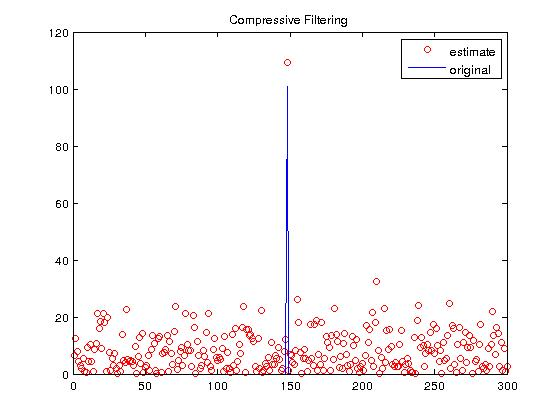
\includegraphics[height = 7.3 cm]{1spike_legend.jpg}
\caption{}
\label{fig:new_basis_25}
\end{figure}
\end{example}
\section{Estimating Frequency Spectra}\label{sec:freq-model}

\subsection{Estimating a single rectangle}

We show how to estimate a signal, composed of a single rectangle \eqref{fig:rectangle} expanded in the following basis

\begin{equation}
l_i\left(x\right) =
\begin{cases}
1 & \text{if } x \leq i \\
0 & \text{ otherwise } 
\end{cases}
\label{basis}
\end{equation}

That is, \(l_i\) is a left-hand step function. 

The basis (\ref{basis}) can be expressed as a matrix in \(\re^{n \times n}\) as:

\begin{equation}
L = \begin{pmatrix}
 1 & 0 & 0 & 0  & 0 \ldots 0 \\
  1 & 1 & 0 & 0  & 0 \ldots 0\\
     1 & 1 & 1 & 0  & 0 \ldots0  \\
    \ldots  \\
     1 & 1 & 1 & 1  & 1 \ldots 1 
\end{pmatrix}
\label{lower-L}
\end{equation}

By direct computation, this inverse of \(L\) is:

\begin{equation}
D = \begin{pmatrix}
 1 & 0 & 0 & 0  & 0 \ldots 0 \\
  -1 & 1 & 0 & 0  & 0 \ldots 0\\
     0 & -1 & 0 & 0  & 0 \ldots0  \\
    \ldots  \\
     0 & 0 & 0 & 0  \ldots -1 & 1
\end{pmatrix}
\label{inv-L}
\end{equation}

We model our PSD signal \(g\) as a linear combination of the basis functions (\ref{basis}):

\begin{equation}
g\left(x\right) = \sum_i a_i l_i\left(x\right) = L^Ta
\label{basis-expansion}
\end{equation}

where \(a = (a_1, \ldots, a_n\) are the coefficients in this basis expansion, and \(l_i\) are the rows of \(L\). Note that as defined, \(g\) is a column vector.

\begin{proposition}
\begin{equation}
D^Tg = a
\end{equation}
\label{def:a}
\end{proposition}
\begin{proof}

\begin{align}
D^Tg &= D^T L^T a \\
&= \left(LD\right)^Ta \\
&= a
\end{align}

as \(LD = I\).

\end{proof}

We define the inner product between two vectors as follows:

\begin{definition}
\begin{equation}
\langle x, y \rangle = x^T y = \sum_i x_i y_i
\end{equation}	
where \(x_i, y_i\) are the components of the vectors \(x,y\) in the \(i^{th}\) direction with respect to some basis vectors \(e_i\).
\end{definition}

We can define a matrix representation for the set of basis vectors \(l_i\), by taking all inner products between all pairs basis vectors:

\begin{definition}
\begin{equation}
F_{n, ij} = \langle l_i, l_j \rangle
\end{equation}

This matrix has the representation:

\begin{equation}
F_{ij} = min(i,j)
\end{equation}

An example of such a matrix is:

\begin{equation}
F_n= \begin{pmatrix}
 1 & 1 & 1 & 1  & 1 \\
  1 & 2 & 2 & 2  & 2\\
     1 & 2 & 3 & 3  & 3  \\
    1 & 2 & 3 & 4  & 4  \\
     1 & 2 & 3 & 4  & 5 
\end{pmatrix}
\label{def:Fmtx}
\end{equation}
\end{definition}

This matrix is invertible.

\begin{theorem}
\begin{equation}
det(F_n) = 1
\end{equation}
\end{theorem}
\begin{proof}
Consider the matrix \(F_n\). Subtract the \(n-1\)th column from the \(n\)th. We obtain a matrix with \(0\) on the final column except the entry \(F_n(n,n) = 1\). Since the top \((n-1) \times (n-1)\) is \(F_{n-1}\) we find that 

\begin{equation}
det(F_n) = 1 \times det(F_{n-1})
\end{equation} 

By recursion and \(det(F_1) = 1\) we have \(det(F_n) = 1\).

\end{proof}

This matrix can be factorised as \(F = LL^T\).

From this it follows that

\begin{equation}
F^{-1} = \begin{pmatrix}
 2 & -1 & 0 & 0  & 0 \ldots 0 \\
  -1 & 2 & -1 & 0  & 0 \ldots 0\\
     0 & -1 & 2 & -1  & 0 \ldots0  \\
    \ldots  \\
     0 & 0 & 0 & 0  \ldots -1 & 1 
\end{pmatrix}
\end{equation}

To find the \(a_i\), we correlate (take the inner product of) the signal against the basis (\ref{basis}).

\begin{definition}
\begin{align}
h_j &= \langle g, l_j \rangle \\
&= \sum_j g\left(x\right) l_j\left(x\right) \\
&= \sum_j a_i l_i\left(x\right) l_j\left(x\right) \\
&= a_i \langle l_i, l_j\rangle \\
&\left(= \sum_{x=1}^j g\left(x\right)\right)
\end{align}

In matrix language \(h = F a^T\). This is the inner product between the signal \(g\) and the basis functions \(l_i\).
\end{definition}

\begin{figure}[h]
\centering
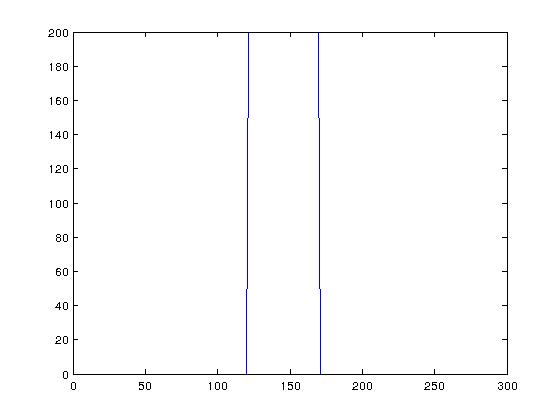
\includegraphics[height = 7.3 cm]{g.jpg}
\caption{}
\label{fig:rectangle}
\end{figure}

Given a set of compressive measurements: 

\begin{equation}
y = Ag
\end{equation}
\\
where \(A \in \re^{m \times n} \), \(A_{ij} \sim \mathcal{N}\left(0,1/m\right)\).
\\
We then compute 
\begin{equation}
\langle y, Al_i\rangle = a_j  l_j^TA^tAl_j \sim \frac{a_j}{m} \langle l_j, l_i \rangle
\end{equation}
for the set of basis vectors \(l_1 \ldots l_n\) i.e. the estimator from the previous section, corresponding to this set of basis functions \eqref{eq: compressive-estimator}. 

We then form the vector 

\begin{equation}
\hat{h} = m \sum_i \langle y, Al_i\rangle l_j \sim h
\label{ss-estimator}
\end{equation}

An example can be seen in figure \ref{fig:hhat}, for a matrix \(A \in \re^{200 \times 300}.\)

\begin{figure}[h]
\centering
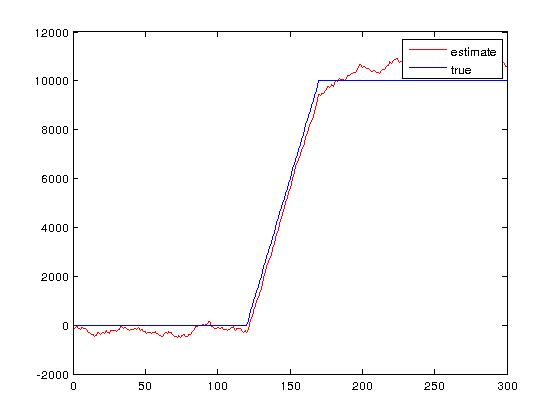
\includegraphics[height = 7.3 cm]{hhat.jpg}
\caption{}
\label{fig:hhat}
\end{figure}

\subsection{Estimating Frequency spectra}

Continuing from the previous (sub)-section we can create an estimate of \(g\), by the following procedure:

\begin{itemize}
\item Estimate the coefficients of the basis \(\hat{a}\) using \(\hat{a} = F^{-1} \hat{h}\)
\item Choose the \(k\) largest (for some \(k\) to be determined later).
\item Between the indices of the \(k\) \(\hat{a}\) take the average of the signal \(L^{-1}\hat{h}\).
\item For each piece between the \(k\) changepoints, do a t-test to determine whether the signal is noise, or a transmission.
\end{itemize}

Some examples of the output of this procedure are shown below, for synthetic and real (Ofcom) data.


\begin{figure}[h]
\centering
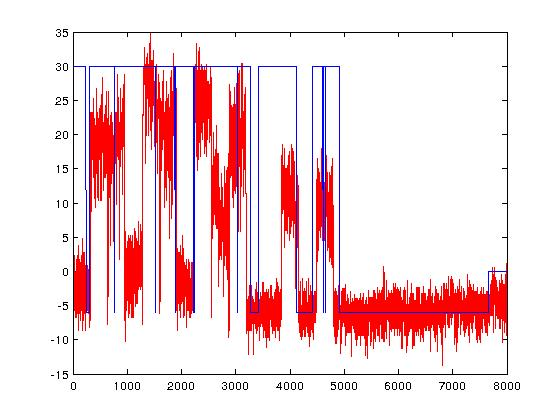
\includegraphics[height = 7.3 cm]{ofcom_classification.jpg}
\caption{}
\label{fig:hvb}
\end{figure}

\begin{figure}[h]
\centering
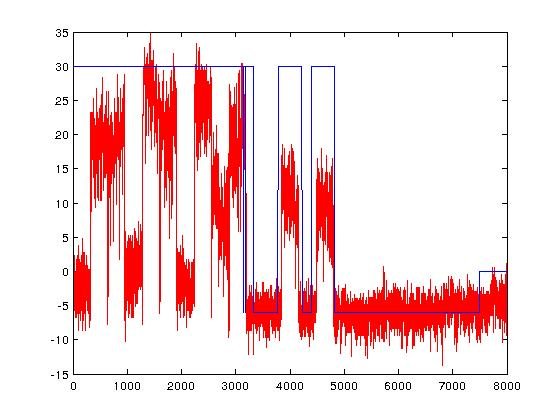
\includegraphics[height = 7.3 cm]{ofcom_classification1.jpg}
\caption{}
\label{fig:hvb}
\end{figure}

\begin{figure}[h]
\centering
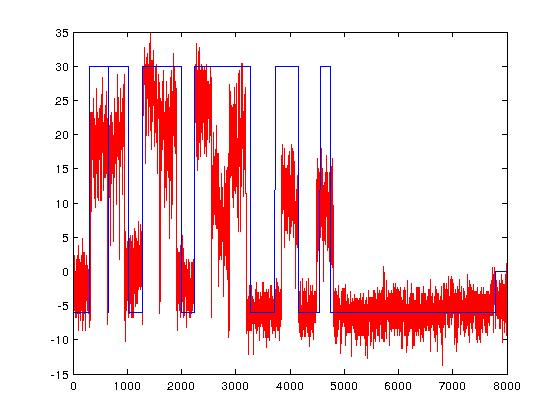
\includegraphics[height = 7.3 cm]{higher_noise_floor0.jpg}
\caption{}
\label{fig:hvb}
\end{figure}

\begin{figure}[h]
\centering
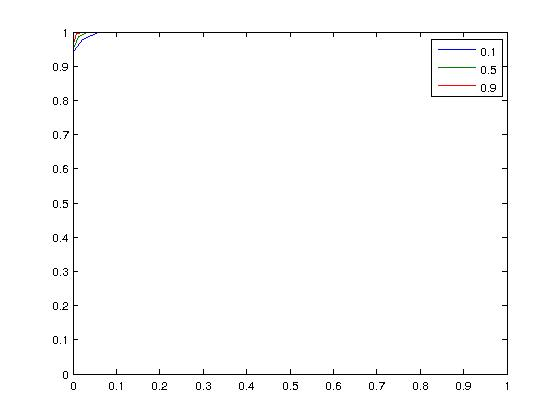
\includegraphics[height = 7.3 cm]{many_roc.jpg}
\caption{}
\label{fig:hvb}
\end{figure}

\section{Time-Frequency Model}
In this section we extend the model from section \ref{sec:freq-model}, to jointly estimate a collection of signals sensed over time. 

In this case, we have a series frequency spectra \(\in \re^n\), sensed at \(T\) time instants. We extend the model, again in the same basis:


\begin{equation}
l_{i,t}\left(x, \tau\right) = \mathbb{I}\left(t \leq \tau \right)\mathbb{I}\left(x \leq i\right)
\label{time-freq basis}
\end{equation}

We can express these basis functions in terms of the basis functions \eqref{basis}, and similarly defined basis functions over time:

\begin{equation}
l_t\left(\tau\right) =
\begin{cases}
1 & \text{if } t \leq \tau \\
0 & \text{ otherwise } 
\end{cases}
\label{time-basis}
\end{equation}

That is, \(l_t\) is again a left-hand step function. 

\begin{proposition}
\begin{equation}
l_{i,t}\left(x, \tau\right) = l_i\left(x\right) \kronecker l_t\left(\tau\right)
\end{equation}
\begin{proof}
Consider a fixed frequency, w.l.o.g \(i=1\). Then 
\begin{equation}
l_{1,t}\left(x, \tau\right) = \mathbb{I}\left(x \leq 1\right)\mathbb{I}\left(t \leq \tau \right)
\end{equation}
There are \(T\) possible vectors, each of length \(n\), for this combination of \(\left(i,t\right)\). Therefore \(l_{1,t}\in \re^{1\times nT} \). As there are \(n\) possible frequency vectors, one for each fixed frequency basis function, we have \(n\times nT\) vectors. By symmetry of time and frequency, the same argument applies for a fixed time, and we have \(T\), \(1\times nT\) basis vectors in total, one for each fixed time instant. Therefore the joint time-frequency basis is in \(\re^{nT \times nT}\). As time and frequency are orthogonal in this representation, the proposition follows.
\end{proof}
\end{proposition}

Thus this basis can be represented with the following matrix:

\begin{equation}
L = L_T \kronecker L_n
\label{def:time-freq matrix}
\end{equation}

where \(L_k\) is the matrix \eqref{lower-L} of size \(k \times k\). From \eqref{def:time-freq matrix}, it follows that:

\begin{equation}
D = L^{-1} = L_T^{-1} \kronecker L_n^{-1} = D_T \kronecker D_n
\end{equation}

where \(D_k\) is the same as \eqref{inv-L}, and that:

\begin{align}
F &= LL^T \\
&= \left(L_n \kronecker L_T\right)\left(L_n \kronecker L_T\right)^T\\
&=L_TL_T^T \kronecker L_nL_n^T \\
&= F_T \kronecker F_n
\end{align}

where \(F_k\) is defined as in \eqref{def:Fmtx}.

We sense the frequency spectrum at \(T\) instants, collecting signals \(g_1, \ldots g_\tau\). 

\begin{definition}
We define
\begin{equation}
G = \left[g_1, \ldots, g_\tau \right]
\end{equation}
and
\begin{equation}
g = \mathrm{vec}\left(G\right) = \dottedcolumn{3}{g_1}{g_\tau}
\end{equation}
\end{definition}

we also define:

\begin{definition}
\begin{equation}
a = \mathrm{vec}\left(a_t\right) = \sum_{t=1}^T e_t \kronecker a_t
\end{equation}
\end{definition}

These definitions are related by the formula:

\begin{equation}
g = L^Ta = \left(L_T^T \kronecker L_n^T\right)a
\end{equation}

We can find an expression for \(a\) by taking the inner product of \(g\) with \(l_{j,s}\):

\begin{align*}
h &= \langle g, l_{j,s}\left(x, \tau\right)\rangle \\
&= \sum_{i,t} g(x,\tau) \langle l_{i,t}, l_{j,s} \rangle \\
&= Fa
\end{align*}

where we have defined \(F = \left(F_T \kronecker F_n\right)\).

The measurements in this model can be written as

\begin{equation}
y_T = A_Tg
\end{equation}

with 

\begin{equation}
A_T = I_T \kronecker A
\end{equation}

and \(A \sim N(0, 1/m)\).

We consider the case where \(g_t = g\) for each time slot (i.e. the signal is unchanging). 

\begin{proposition}
We can write the \(i^{th}\) column of the matrix \(L_k\) as, for \(k \leq j\):

\begin{equation}
L_k^T e_i = \sum_{j=1}^i e_j
\end{equation}

where \(e_j\) is the \(j^{th}\) canonical basis vector in \(\re^k\), with has a \(1\) in position \(j\) and is zeros everywhere else.

\begin{proof}
The \(i^{th}\) column of \(L_k\) will have \(i\) ones, and \(k-i\) zeros. It can be written in terms of the canonical basis \(e_j\), simply as sum up to the last \(1\) in position \(i\).
\end{proof}

\end{proposition}

In this case, we can write \(g\) as:

\begin{align*}
g = L^T a &= \left(L_T^T \kronecker L_n^T\right)\left(\sum_{t=1}^T e_t \kronecker a_t\right) \\
&= \sum_{t=1}^T L_T^T e_j \kronecker L_n^Ta_t \\
&= \sum_{t=1}^T \left(\sum_{j=1}^n e_j \right) \kronecker L_n^T a_t \\
&= \sum_{j=1}^T e_j \kronecker \sum_{t=j}^T L_n^T a_t \\
&= \sum_{j=1}^T e_j \kronecker b_j
\end{align*}

where we define \(b_j = \sum_{t=j}^T L_n^T a_t\). We can now write

\begin{align*}
y_T = A_Tg &= \left(I_T \kronecker A \right) \left(\sum_{j=1}^T e_i \kronecker b_j\right)\\
&= \sum_{j=1}^T e_j \kronecker Ab_j
\end{align*}

\begin{example}
Now consider the case where all the \(a_t\) are identical. In this case:

\begin{equation}
\twopartdef{a_T = a}{t=T}{a_t = 0}{t < T}
\end{equation}

so

\begin{equation}
b_j = \sum_{t=j}^T L_n^T a_t = L_n^T a = b
\end{equation}

Then

\begin{equation}
y_T = \left( \sum_{j=1}^T \right) \kronecker Ab = 1_T \kronecker Ab
\end{equation}
\end{example}

Let the \(s^{th}\) column of \(L_T^T\) be denoted by \(B_s\), then

\begin{align*}
\left(L_T^T\right)^{-1}B_s = D_T^T B_s = e_s
\end{align*}



As before, we form the estimator

\begin{align*}
\hat{h}_T = \sum_{i,t} \langle y_T, A_T l_{i,t} \rangle l_{i,t} \sim \frac{1}{mT} Fa
\end{align*}

and run the algorithm defined in the last section on the results.

Consider 

\begin{align*}
\langle y_T, A_T l_{i,t} \rangle &= \langle A_T^T y_T,l_{i,t} \rangle \\
&= \langle \left(I_T \kronecker A^T\right)\left(\sum_{j=1}^T e_j \kronecker Ab_j\right), \left(l_t \kronecker l_i\right)\rangle \\
&= \langle \sum_{j=1}^T e_j \kronecker A^TAb_j, \left(l_t \kronecker l_i\right)\rangle \\
&= \sum_{j=1}^T e_j^T l_t \kronecker b_j^TA^TAl_i \\
&\sim \frac{1}{m}\sum_{j=1}^T e_j^T l_t \kronecker b_j^Tl_i\\
&\stackrel{?}{=} \frac{1}{m}\sum_{j=1}^T j \kronecker F_n a
\end{align*}

where we used the expectation of a Wishart matrix between the \(5^{th}\) and \(6^{th}\) lines.

\begin{figure}[h]
\centering
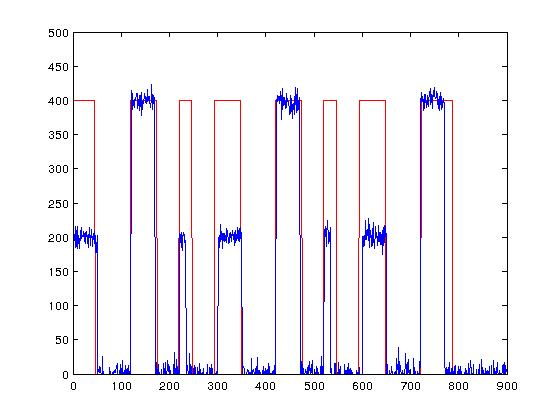
\includegraphics[height = 7.3 cm]{time_freq_model.jpg}
\caption{}
\label{fig:hvb}
\end{figure}

\begin{figure}[h]
\centering
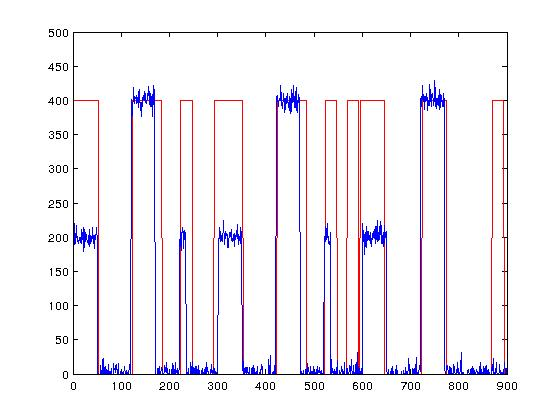
\includegraphics[height = 7.3 cm]{time_freq_1.jpg}
\caption{}
\label{fig:hvb}
\end{figure}

\begin{figure}[h]
\centering
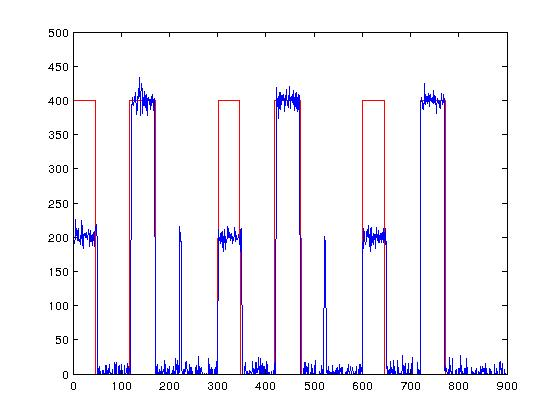
\includegraphics[height = 7.3 cm]{time_freq_missing.jpg}
\caption{}
\label{fig:hvb}
\end{figure}


\bibliography{cswireless2}
\end{document}
\documentclass[conference]{IEEEtran}

\usepackage{cite}
\usepackage[cmex10]{amsmath}
\usepackage{amsfonts,amssymb}
\usepackage[pdftex]{graphicx}
\usepackage[algoruled]{algorithm2e}
%usepackage{titlesec}
\usepackage{graphicx}

\bibliographystyle{IEEEtran}


%\usepackage{amsmath,amsfonts,amssymb,latexsym,amsthm,verbatim,a4wide}


 %\theoremstyle{plain}
  \newtheorem{theorem}{Theorem}[section]
  \newtheorem{corollary}[theorem]{Corollary}
  \newtheorem{proposition}[theorem]{Proposition}
  \newtheorem{lemma}[theorem]{Lemma}
\newtheorem{example}[theorem]{Example}
  \newtheorem{definition}[theorem]{Definition}
  \newtheorem{conj}[theorem]{Conjecture}
 \newtheorem{condition}{Condition}
 \newtheorem{remark}[theorem]{Remark}

\newcommand{\vc}[1]{{\mathbf{ #1}}}
\newcommand{\tn}{\widetilde{\nabla}_{n} }
\newcommand{\Z}{{\mathbb{Z}}}
\newcommand{\re}{{\mathbb{R}}}
\newcommand{\II}{{\mathbb{I}}}
\newcommand{\ep}{{\mathbb{E}}}
\newcommand{\pr}{{\mathbb{P}}}
\newcommand{\FF}{{\mathcal{F}}}
\newcommand{\TT}{{\mathcal{T}}}
\newcommand{\phin}{\phig{n}}
\newcommand{\phig}[1]{\phi^{(#1)}}
\newcommand{\ol}[1]{\overline{#1}}
\newcommand{\eff}{{\rm eff}}
\newcommand{\suc}{{\rm suc}}
\newcommand{\tends}{\rightarrow \infty}
\newcommand{\setS}{{\mathcal{S}}}
\newcommand{\setP}{{\mathcal{P}}}
\newcommand{\setX}{{\mathcal{X}}}
\newcommand{\nec}{{\rm nec}}
\newcommand{\bd}{{\rm bd}}

\begin{document}

\title{The capacity of non-identical adaptive group testing}
\date{\today}
\author{\IEEEauthorblockN{Tom Kealy} \IEEEauthorblockA{CDT in Communications   \\ MVB, School of Engineeering \\ University of Bristol, UK \\ Email: tom.kealy.kealy@bristol.ac.uk}
\and \and 
\IEEEauthorblockN{Oliver Johnson} \IEEEauthorblockA{School of Mathematics\\ University Walk, Bristol \\
University of Bristol, UK \\ Email: O.Johnson@bristol.ac.uk}
\and
\IEEEauthorblockN{ Robert Piechocki} \IEEEauthorblockA{CSN Group \\ MVB, School of Engineeering \\ University of Bristol, UK \\
Email: r.j.piechocki@bristol.ac.uk}
}
\maketitle

\begin{abstract}
\noindent We consider the group testing problem, in the case where the items are defective independently but with non-constant probability.
We introduce and analyse an algorithm to solve this problem by grouping items together appropriately. We give conditions under which  the
algorithm performs essentially optimally in the sense of information-theoretic capacity.
This has applications to the allocation of spectrum to cognitive radios, in the case where a database gives prior information that a particular band will be occupied.
\end{abstract}



\section{Introduction and notation}

\subsection{The Probabilistic group testing problem}
Group testing is a sparse inference problem, first introduced by Dorfman \cite{dorfman} in the context of testing for rare diseases.
Given  a large population of items $\setP$,
indexed by \( \{1, \ldots N\}\), where
some small fraction of the items are interesting in some way, how can we find the interesting items efficiently? 

We perform a sequence of $T$ pooled tests defined by test sets $\setX_1, \ldots, \setX_T$, where each $\setX_i \subseteq \setP$. 
We represent the interesting (`defective') items by 
a random vector $\vc{U} = ( U_1, \ldots, U_N)$, where $U_i$ is the indicator of the event that item $i$ is defective. 
For each test $i$, we jointly 
test all the items in $\setX_i$, and the outcome $y_i$ is `positive' ($y_i = 1$) if and only if any item in $\setX_i$ is defective. In other words, 
$y_i = \II \left( \sum_{j \in \setX_i} U_j \right)$, since for simplicity we are  considering the noiseless case. Further, in this paper, we restrict our attention to
 the adaptive case, where we choose test set
$\setX_i$ based on a knowledge of sets $\setX_1, \ldots, \setX_{i-1}$ and outcomes $y_1, \ldots, y_{i-1}$. The group testing problem requires us to infer $\vc{U}$ with high
probability given a low number of tests $T$.

Since Dorfman's paper \cite{dorfman}, there has been considerable work on the question of how to design the sets $\setX_i$ in order to minimise the number of tests $T$
required. In this context, we briefly mention so-called combinatorial designs (see \cite{du, malyutov} for a summary, with \cite{malyutov} giving invaluable
references to an extensive body of Russian work in the 1970s and 1980s). Such designs typically aim to ensure that 
set-theoretic properties known as disjunctness
and separability occur. In contrast, for simplicity of analysis, as well as  performance of optimal order, it is possible to consider random designs. Here sets $\setX_i$ are chosen
at random, either using constructions such as independent Bernoulli designs \cite{atia, johnsonc8, johnson33} or more sophisticated  random designs based on LDPC codes \cite{wadayama}. 

Much previous work has focussed on the Combinatorial group testing problem, where there are a fixed number of defectives $K$, and the defectivity vector $\vc{U}$ is chosen uniformly among all
binary vectors of weight $K$. In contrast, in this paper we study a Probabilistic group testing problem as formulated
for example in the work of Li et al. \cite{li5}, in that we suppose 
 each item is defective  independently with probability \(p_i\), or equivalently take $U_i$ to be independent Bernoulli($p_i$).

This Probabilistic framework, including non-uniform priors, is natural for many applications of group testing.
For example, see \cite{atia2}, the cognitive radio problem can be formulated in terms of  a population
 of communication bands in frequency spectra with some (unknown) occupied bands you must not utilise. Here, the values of $p_i$ may be chosen
 based on some database of past spectrum measurements or other prior information. Similarly, as in Dorfman's original work  \cite{dorfman} or more recent 
research \cite{shental} involving screening for genetic conditions, values of
$p_i$ might summarise prior information based on a risk profile or  family history.
%
\subsection{Group testing capacity}
%
It is possible to characterize performance tradeoffs in group testing 
 from an information-theoretic point of view -- see for example \cite{atia, johnsonc10, johnson33, tan}. These papers have focussed on group testing as a channel coding problem, 
with \cite{atia, tan}
explicitly calculating the mutual information.
The paper \cite{johnsonc10} defined the capacity of a Combinatorial group testing procedure, which characterizes the number of bits of information
about the defective set which we can learn per test. We give a more general definition here,
which covers both the Combinatorial and Probabilistic cases.
%
\begin{definition} \label{def:capacity} Consider a sequence of group testing problems where the $i$th problem
has defectivity vector  $\vc{U}^{(i)}$, and consider algorithms which are given $T(i)$ tests.
We refer to a constant $C$ as the (weak) group testing capacity if for any $\epsilon > 0$:
  \begin{enumerate}
    \item any sequence of algorithms with
      \begin{equation} \label{eq:lower}
        \liminf_{i \tends} \frac{ H(\vc{U}^{(i)}) }{T(i)} \geq C+ \epsilon,
      \end{equation}
      has success probability $\pr(\suc)$ bounded away from 1,
    \item and there exists a sequence of algorithms with
      \begin{equation} \label{eq:upper}
        \liminf_{i \tends} \frac{H(\vc{U}^{(i)}) }{T(i)}  \geq C - \epsilon
      \end{equation}
      with success probability $\pr(\suc) \rightarrow 1$.
  \end{enumerate}
\end{definition}
%
\begin{remark}
In the Combinatorial case of $K$ defective items with all defective sets equally
likely, $ H(\vc{U}) = \log_2 \binom{N}{K}$, which is the term found in the denominator in \cite[Eq. (1) and (2)]{johnsonc10}. In the Probabilistic case (as in \cite{li5}) 
 we know $H(\vc{U}) = -\sum_{i=1}^N h(p_i)$ where $h(t) = -t \log_2 t - (1-t) \log_2(1-t)$ is the binary entropy function. 
\end{remark}
%
\begin{remark} If for $ \liminf_{i \tends} \frac{ H(\vc{U}^{(i)}) }{T(i)} \geq C+ \epsilon$, the success probability 
$\pr(\suc) \rightarrow 0$ we say that $C$ is the strong group testing capacity, following standard terminology in information
theory. Such a result is referred to as a strong converse.
\end{remark}

\subsection{Main results}

The principal contribution of \cite[Theorem 1.2]{johnsonc10} was the following result:
%
\begin{theorem}[\cite{johnsonc10}] \label{thm:mainold}
The strong capacity of the adaptive noiseless Combinatorial group testing problem
  is  $C = 1$,
  in any regime such that $K/N \rightarrow 0$.
\end{theorem}
%
This argument came in two parts. First, in \cite[Theorem 3.1]{johnsonc10} the authors  proved a new
upper bound on success probability 
\begin{equation} \label{eq:bja} \pr(\suc) \leq \frac{2^T}{\binom{N}{K}}, \end{equation} which implied a strong converse ($C \leq 1$). This was complemented 
by 
showing that, in the Combinatorial case, an algorithm based on 
Hwang's Generalized Binary Splitting Algorithm (HGBSA) \cite{hwang}, \cite{du} is essentially optimal in the required sense,
showing that $C=1$ is achievable.


It may be useful to characterize the Probabilistic group testing problem in 
terms of the effective sparsity $\mu^{(N)}: = \sum_{i=1}^N p_i$. In particular, if the $p_i$ are (close to) identical, we would expect performance similar to that in the Combinatorial
case with $K = \mu^{(N)}$ defectives. As in \cite{johnsonc10}, we  focus on asymptotically sparse cases, where $\mu^{(N)}/N \rightarrow 0$ (in contrast, Wadayama
\cite{wadayama} considered a model where $p_i$ are identical and fixed).
The main result of the present paper is Theorem \ref{thm:main}, stated and proved in Section \ref{sec:main} below, which implies the 
following  Probabilistic group testing version of Theorem \ref{thm:mainold}.
 %
\begin{corollary} \label{cor:main}
 In the case where $p_i \equiv p$, the weak capacity of the adaptive noiseless Probabilistic group testing problem
  is  $C = 1$, in any regime such that $\mu^{(N)}/N \rightarrow 0$ and $\mu^{(N)} \rightarrow \infty$.
  \end{corollary}



Again we prove our main result Theorem \ref{thm:main} using complementary bounds on both sides. First in Section \ref{sec:ub} we recall
 a universal upper bound on success probability, Theorem \ref{thm:upper}, taken from
\cite{li5}, which implies a weak converse.   In \cite{li5}, Li et al. introduce
the Laminar Algorithm for Probabilistic group testing.  
In Section \ref{sec:algo} we propose a refined version of this Laminar Algorithm, based on Hwang's HGBSA \cite{hwang}, which is
analysed in Section \ref{sec:main}, and shown to imply performance close to optimal in the sense of capacity.

\section{Algorithms and existing results}

\subsection{Upper bounds on success probability} \label{sec:ub}

Firstly \cite[Theorem 1]{li5} can be restated to give the following
upper bound on success probability:
%
\begin{theorem} \label{thm:upper}
Any Probabilistic group testing algorithm using $T$ tests with noiseless measurements has success probability satisfying
$$ \pr(\suc) \leq \frac{T}{H( \vc{U})}.$$
\end{theorem}

Rephrased in terms of Definition \ref{def:capacity}, this tells us that the weak capacity of noiseless Probabilistic 
group testing is $\leq 1$. The logic is as follows; if the capacity were
$1 + 2 \epsilon$ for some $\epsilon > 0$, then there would exist a sequence of algorithms with $H(\vc{U}^{(i)})/T(i) \geq 1 + \epsilon$ with success probability tending to 1.
However, by Theorem \ref{thm:upper}, any such algorithms have $\pr(\suc) \leq 1/(1+\epsilon)$, meaning that we have 
established that a weak converse holds.

\begin{remark}
It remains an open and interesting problem to prove an equivalent of \eqref{eq:bja} as in \cite[Theorem 3.1]{johnsonc10}. That is we hope to find an upper bound
on success probability in a form  which implies a strong converse, and hence that the strong capacity of Probabilistic group
testing is equal to 1.
\end{remark}

\subsection{Binary search algorithms}

The main contribution of this work is  to describe and analyse algorithms that will find the defective items.
In brief, we can think of Hwang's HGBSA algorithm as dividing the population $\setP$ into search sets $\setS$. First, all the items in a search set $\setS$ are tested together,
using a test set $\setX_1 = \setS$. If the result is negative
($y_1 = 0$), we can be certain that $\setS$ contains no defectives. However, if the result is positive ($y_1 = 1$),  $\setS$ must contain at least one defective.

If $y_i = 1$, we can be guaranteed to find at least
one defective, using the following binary search strategy.  
We  split the   set $\setS$ in two, and test the `left-hand' set, say $\setX_{2}$. If $y_{2} = 1$, then we know that $\setX_{2}$ contains at least one defective.
If $y_{2} = 0$, then $\setX_{2}$ contains no defective, so we can deduce that $\setS \setminus \setX_2$ contains at least one defective. By repeated use of this strategy, we are 
guaranteed to find a succession of nested sets which contain at least one defective, until $\setX_i$ is of size 1, and we have isolated a single defective item.

However this strategy may not find every defective item in $\setS$. To be specific, it is possible that at some stage
both the left-hand and right-hand sets contain a defective. The Laminar Algorithm of \cite{li5} essentially deals with this by testing 
both sets. However, we believe that this is inefficient, since typically both sets will not contain a defective. Nonetheless, the Laminar Algorithm satisfies
 the following  performance guarantees  proved in \cite[Theorem 2]{li5}: 
%
\begin{theorem} \label{thm:lower}
The expected number of tests required by the Laminar Algorithm \cite{li5}  is $\leq 2 H(\vc{U}) + 2 \mu$. Under a technical condition (referred to as non-skewedness), the
success probability can be bounded by $\pr(\suc) \geq 1- \epsilon$ using $T = (1+ \delta) (2^{\Gamma + \log_2 3} + 2) H(\vc{U})$ tests, where $\Gamma$ is defined implicitly
in terms of $\epsilon$, and $\delta \geq 2 e - 1$.
\end{theorem}

Ignoring the $\Gamma$ term, and assuming the non-skewedness condition holds,
 this implies that (using the methods of \cite{li5}) $T =  2 e (3 + 2) H(\vc{U}) = 10 e H(\vc{U})$ tests are required to guarantee convergence to $1$
of the success probability. In our language, this implies a lower bound of $C \geq 1/(10 e) = 0.0368$. Even ignoring the analysis of error probability, the fact that the expected number
of tests is $\leq 2 H(\vc{U}) + 2 \mu$ suggests that we cannot hope to achieve $C > 1/2$ using the Laminar Algorithm.
%
\subsection{Summary of our contribution} \label{sec:algo}

\begin{algorithm}
 \SetLine 
 %\SetAlgoLined % For previous releases [?]
 \KwData{A Set \(S\) of \(\lvert S \rvert = n\) items, \(\mu\) of which are actually defective in expectation, a probability vector \( \vec{p}^{\left(n\right)} \) describing each item's independent probability of being defective, and a cutoff \(\theta\)}
 \KwResult{The set of defective items}
 Discard items with \(p_i \leq \theta\)
 \\
 Sort the remaining items into \(B\) bins, collecting items together with \(p_i \in \left[1/2C^r,1/2C^{r-1}\right)\) in bin \(r\).
 \\
 Sort the items in each bin into sets s.t. the (normalised) probability of each set is less than \(1/2\).
 \\
 Test each set in turn
 \\
   	\If{The test is positive}{Arrange the items in the set on a Shannon-Fano/Huffman Tree and search the set for all the defectives it contains}

 \caption{Algorithm for the non-iid group testing problem}
\end{algorithm}

The main contribution of our paper is a refined version of the Laminar Algorithm, summarised above, and an analysis resulting in tighter error bounds as formulated in Proposition \ref{prop:overall} (in terms of expected number of tests) and Theorem \ref{thm:main} (in terms
of error probabilities).
The  key ideas are:
\begin{enumerate}
\item To partition the population $\setP$ into search  sets  $\setS$ containing items which have similar probabilities,
expressed through the Bounded Ratio Condition \ref{cond:ratio}. This is discussed in Section \ref{sec:boundedratio}, and optimised in the proof
of Proposition \ref{prop:overall}.
\item The way in which we deal with sets $\setS$ which contain more than one defective, as discussed in Remark \ref{rem:algo} below. Essentially we do not backtrack after each test by
testing both left- and right-hand sets, but only backtrack after each defective is found.
\item To discard items which have probability below a certain
threshold, since with high probability none of them will be defective. This is an idea introduced in \cite{li5} and discussed
in Section \ref{sec:discard}, with a new bound given in Lemma \ref{lem:thresh}.
\item  Careful analysis in Section \ref{sec:expectation} of the properties of search sets $\setS$ gives Proposition \ref{prop:overall}, which shows that the expected number of tests required can
be expressed as $H(\vc{U})$ plus an error term. In Section \ref{sec:main},
we give an analysis of the error probability using Bernstein's inequality, Theorem \ref{thm:bernstein}, allowing us to
prove Theorem \ref{thm:main}.
\end{enumerate}
%


\subsection{Wider context: sparse inference problems}

Recent work \cite{aksoylar,tan} has shown that many arguments and bounds hold in a common framework of sparse inference
which includes group testing and compressive sensing.

Digital communications, audio, images, and text are examples of data sources we can compress. We can do this, because these data sources are sparse: they have fewer degrees of freedom than the space they are defined upon. 
For example, images have a well known expansion in either the Fourier or Wavelet bases. The text of an English document will only be comprised of words from the English dictionary, and not all the possible strings from the space of strings made up from the characters \(\{a, \ldots, z \}\). 

Often, once a signal has been acquired it will be compressed. However, the compressive sensing paradigm introduced by
\cite{candes,donoho2} shows that this isn't necessary. In those papers it was shown that a 'compressed' representation of a signal could be obtained from random linear projections of the signal and some other basis (for example White Gaussian Noise). The question remains, given this representation how do we recover the original signal? For real signals, a simple linear programme suffices.
Much of the work in this area has been couched in terms of the sparsity of the signal and the various bases the signal can be represented in (see for example \cite{candes,donoho2}). 


\section{Analysis and new bounds}

\subsection{Searching a set of bounded ratio} \label{sec:boundedratio}

Recall that we have a population $\setP$ of items to test, each with associated probability of defectiveness $p_i$.
The strategy of the proof is to partition $\setP$ 
 into search sets $\setS_1, \ldots, \setS_G$, each of which contains items which have
comparable values of $p_i$.

\begin{condition}[Bounded Ratio Condition] \label{cond:ratio}
Given $C \geq 1$, say that a set $\setS$ satisfies the Bounded Ratio Condition with constant $C$ if
\begin{equation} \label{eq:ratio} \max_{i,j \in \setS} \frac{p_j}{p_i} \leq C.\end{equation} \end{condition}
%
(For example clearly if $p_i \equiv p$, any set $\setS$ satisfies the condition for any $C \geq 1$).
%
\begin{lemma} \label{lem:sfstep}
Consider a set $\setS$ satisfying the Bounded Ratio Condition  with constant $C$
and write $P_{\setS} = \sum_{j \in \setS} p_j$.
In a  Shannon--Fano tree for the probability distribution $\ol{p}_i := p_i/P_{\setS}$, each item has length $\ell_i^{(\setS)}$
bounded by
\begin{equation} \label{eq:depth} \ell_i^{(\setS)} \leq \ell_{\max}^{(\setS)} := \frac{h(\setS)}{P_{\setS}} + \log_2  C + \log_2  P_{\setS} + 1,\end{equation}
where we write $h( \setS) :=  -\sum_{j \in \setS} p_j \log_2  p_j$.
\end{lemma}
\begin{IEEEproof} Under the Bounded Ratio Condition, for any $i$ and $j$, we know that by taking logs of \eqref{eq:ratio}
$$ -\log_2 p_i \leq - \log_2 p_j + \log_2 C.$$
Multiplying by $p_j$ and summing over all $j \in \setS$, we obtain that
\begin{equation} \label{eq:setbd} -P_{\setS} \log_2 p_i \leq h(\setS) + P_{\setS} \log_2 C.\end{equation}
Now, the Shannon--Fano length of the $i$th item is
\begin{eqnarray}
 \ell_i^{(\setS)}  = \lceil -\log_2 \ol{p}_i \rceil 
& \leq &  -\log_2 p_i + \log_2 P_{\setS} + 1 \label{eq:lengthbd} \\
& \leq  & \left(\frac{h(\setS)}{P_{\setS}} + \log_2 C \right) + \log_2 P_{\setS} + 1. \nonumber
\end{eqnarray}
and the result follows by \eqref{eq:setbd}.
\end{IEEEproof}

Next we describe our search strategy:

\begin{remark} \label{rem:algo}
Our version of the algorithm will find every defective in a set $\setS$. We start as before by testing every item in $\setS$ together. If this test is negative, we are done.
Otherwise, if it is positive, we can perform binary search as above to find one defective item, say $d_1$. Now, test every item in $\setS \setminus \{ d_1 \}$ together.
If this test is negative, we are done, otherwise we repeat the search step on this smaller set, to find another defective item
$d_2$, then we test $\setS \setminus \{ d_1, d_2 \}$ and so on.

We think of the algorithm as repeatedly searching a binary tree. Clearly, if the tree has depth bounded by $\ell$, then the search will take $ \leq \ell$ tests to find one defective. In total, 
if the set contains $U$ defectives, we need to repeat $U$ rounds of searching, plus the final test to guarantee that the set contains no more defectives, so will use $\leq \ell U + 1$ tests.
\end{remark}

\begin{lemma} \label{lem:expset}
 Consider a search set $\setS$ satisfying the Bounded Ratio Condition  and write $P_{\setS} = \sum_{j \in \setS} p_j$.
If (independently) item $i$ is defective with probability $p_i$, 
we can recover  all defective items in the set using $T_\setS$ tests, where $\ep T_\setS \leq T_{\bd}(\setS)$ for
\begin{equation} \label{eq:tbds}
 T_{\bd}(\setS) :=  h(\setS) +  P_{\setS} \log_2 C +  P_{\setS} \log_2 P_{\setS} + P_\setS + 1. \end{equation}
\end{lemma}
\begin{IEEEproof}
Using the algorithm of Remark \ref{rem:algo}, laid out on the Shannon-Fano tree constructed in Lemma \ref{lem:sfstep}, we are guaranteed  to find every defective.
The number of tests to find one defective thus corresponds to the depth of the tree, which is bounded by  $\ell_{\max}^{(\setS)}$ given in \eqref{eq:depth}.

Recall that we write $U_i$ for the indicator of the event that the $i$th item is defective, $U_{\setS} = \sum_{i \in \setS} U_i$ and 
$l_i^{(\setS)}$ for the length of the word in the Shannon Fano tree. As discussed in Remark \ref{rem:algo}
this search procedure will take 
\begin{eqnarray}
T_\setS & = &  1 + \sum_{i \in \setS} U_i \ell_i^{(\setS)} \nonumber \\
& = &  \sum_{i \in \setS} p_i \ell_i^{(\setS)} + 1 + \sum_{i \in S} \ell_i^{(\setS)} (U_i - p_i)  \nonumber \\
& \leq & \sum_{i \in \setS} p_i \ell_{\max}^{(\setS)} +  1 + \sum_{i \in \setS} V_i^{(\setS)}  \nonumber \\
& =  &  P_{\setS} \ell_{\max}^{(\setS)} +  1 + \sum_{i \in S} V_i^{(\setS)} \nonumber \\
& \leq  & T_{\bd}(\setS) + \sum_{i \in S} V_i^{(\setS)} 
\mbox{ \;\; tests.} \label{eq:testsperdef} \end{eqnarray}
Here we write $V_ i^{(\setS)} = \ell_i^{(\setS)} (U_i - p_i)$, which has expectation zero, and \eqref{eq:testsperdef} follows using the expression for 
$\ell_{\max}^{(\setS)}$ given in   Lemma \ref{lem:sfstep}.
\end{IEEEproof}

\subsection{Discarding low probability items} \label{sec:discard}

As in \cite{li5}, we use a probability threshold $\theta$, and write $\setP^*$ for the population having removed items with $p_i \leq \theta$.
If an item lies in $\setP \setminus \setP^*$ we do not 
test it, and simply mark it as non-defective. This truncation operation gives an error if and only if some item in $\setP \setminus \setP^*$ is defective.
By the union bound, 
this truncation operation contributes a total of $\pr( \mbox{$\setP \setminus \setP^*$ contains a defective}) \leq  \rho := \sum_{i=1}^n p_i \II(p_i \leq \theta)$ to the error probability.



\begin{lemma} \label{lem:thresh}
Choosing $\theta(P_e)$ such that  
\begin{equation} \label{eq:thetadef}
-\log_2 \theta(P_e) = \min\left( \log_2  \left( \frac{2n}{P_e} \right), \frac{2 H( \vc{U})}{P_e} \right)
\end{equation}
ensures that  
\begin{equation}
\pr( \mbox{ $\setP \setminus \setP^*$ contains a defective} ) \leq P_e/2. \label{eq:setpstar} \end{equation} \end{lemma}
\begin{IEEEproof}
The approach of \cite{li5} is essentially to bound $\II(p_i \leq \theta) \leq \theta/p_i$ so that
$\rho = \sum_{i=1}^n p_i \II(p_i \leq \theta) \leq \sum_{i=1}^n p_i (\theta/p_i) = n \theta$. Hence, choosing a threshold
of $\theta = P_e/(2n)$ guarantees the required bound on $\rho$.

We combine this with another bound, constructed using a different function:
 $\II(p_i \leq \theta) \leq (-\log_2 p_i)/(-\log_2 \theta)$, so that
$$ \rho = \sum_{i=1}^n p_i \II(p_i \leq \theta) \leq \sum_{i=1}^n p_i  \left( 
\frac{-\log_2 p_i}{-\log_2 \theta } \right) \leq \frac{H( \vc{U})}{-\log_2 \theta},$$ 
so we deduce the result. \end{IEEEproof}

\subsection{Searching the entire set} 

Having discarded items with $p_i$ below
this probability threshold $\theta$ and given bounding ratio $C$,
we create a series of bins. We collect together items with probabilities $p \in [1/2,1]$ in bin 0,
$p \in [1/(2C), 1/2)$ in bin 1, items with probabilities $p \in [1/(2C^2), 1/(2C))$ in bin 2, \ldots, and items with probabilities $p \in 
[1/(2C^B), 1/(2C^{B-1}))$ in bin $B$.

The probability threshold $\theta$ means that
there will be a finite number of such bins, with the index $B$ of the last bin defined by the fact that $1/(2C^B) \leq
\theta < 1/(2C^{B-1})$, meaning that $(B -1) \log_2 C < - \log_2 (2 \theta)$, so
\begin{equation} \label{eq:bincount} B \leq  \frac{ - \log_2 (2 \theta)}{\log_2 C} + 1. \end{equation}

We split the items in each bin into search sets $\setS_i$, motivated by the following definition:

\begin{definition} \label{def:full}
A set of items \( \setS \) is said to be full if $P_{\setS} = \sum_{i \in \setS} p_i \geq \frac{1}{2}$.
\end{definition}

Our splitting procedure is as follows: we create a list of
possible sets $\setS_1, \setS_2, \ldots $. For $i$ increasing from $0$ to $B$,
we place items from bin $i$ into sets $\setS_{b_{i}+1}, \ldots, \setS_{b_{i+1}}$, for some $b_i$, where $b_{0} = 0$.
Taking the items 
from bin $i$, while $\setS_{b_{i}+1}$ is not full  (has 
total probability $< \frac{1}{2}$) we will place  items into it. Once enough items have been added to fill $\setS_{b_{i} + 1}$,
we will proceed in the same way to fill $\setS_{b_{i}+2}$, and so on until all the items in bin $i$ have been
assigned to sets $\setS_{b_{i}+1}, \ldots, \setS_{b_{i+1}}$,  where $\setS_{b_{i+1}}$ may remain not full.
%
\begin{proposition} \label{prop:splitting}
 This splitting procedure will divide $\setP^*$ into search sets $\setS_1, \ldots, \setS_G$, where
the total number of sets is 
$$ G \leq 2 \mu + B \leq 2 \mu  +  \left( \frac{ -\log_2 (2\theta)}{\log_2 C} + 1 \right).$$ 
Each set $\setS_j$ satisfies the Bounded Ratio Condition and has total probability $P_j := P_{\setS_j} \leq 1$. \end{proposition}
\begin{IEEEproof}
First, note that  
the items from bin $0$ each lie in a set $\setS$ on their own.
These sets will be full, trivially satisfy the Bounded Ratio Condition \ref{cond:ratio}
with constant $C$,
 and have probability satisfying $P_j \leq 1$.
 For each of bins $1, \ldots, B$:
\begin{enumerate}
\item  \label{it:count} For each bin $i$,
it is possible that the last set $\setS_{b_{i}+1}$  will not be full, but every other
set corresponding to that bin will be full. Hence, there are no more than $B$ sets which are not full.
\item For each resulting set $\setS_j$, the total probability $P_j \leq 1$ (since just before we add the final item, $\setS_j$ is not full, so at
that stage has total probability $\leq 1/2$, and each element in bins $1, \ldots, B$ has probability $\leq 1/2$).
\item Since each set $\setS_j$ contains items  taken from the same bin, it will satisfy the Bounded Ratio Condition  with 
constant $C$.
\end{enumerate}

 Note that the number of full sets is \(\leq 2 \mu \), since
\begin{equation} \label{eq:counting}
\mu =  \sum_{i \in \setP} p_i \geq \sum_{i \in \setP^*} p_i  = \sum_{j=1}^G P_j
\geq
\sum_ {\mbox{\scriptsize $j$: $\setS_j$ full}} P_j \geq \left| \mbox{$\setS_j$ full} \right| \frac{1}{2}. \end{equation}
Since, as discussed  in point \ref{it:count}) above,
 the total number of sets is bounded by the number of full sets plus $B$, the result follows using Equation
(\ref{eq:bincount}).
\end{IEEEproof}

\subsection{Bounding the expected number of tests} \label{sec:expectation}
%
We allow the algorithm to work until all defectives in $\setP^*$ are found, and write $T$ for the (random) number of tests this takes.
%
\begin{proposition} \label{prop:overall} Given a population $\setP$
where (independently) item $i$ is defective with probability $p_i$,  
we  recover  all defective items in $\setP^*$ in $T$ tests with $\ep T \leq T_{\bd}$, where
\begin{equation} \label{eq:tbd}
 T_{\bd} := \left( H( \vc{U}) + 3 \mu + 1 \right) +  
 2 \sqrt{ \mu  \left( -\log_2 (2\theta) \right)}.
\end{equation}
\end{proposition}
\begin{IEEEproof} Given a value of $C$,
Proposition \ref{prop:splitting} shows that our splitting procedure divides $\setP^*$ into 
$G$ sets $\setS_1, \ldots, \setS_G$, such that each set $\setS_j$ satisfies the Bounded Ratio Condition with constant $C$ and has total probability $P_j
\leq 1$. Using the notation of Lemma \ref{lem:expset}, $T = \sum_{j=1}^G T_{\setS_j}$, where 
$\ep T_{\setS_j} \leq  T_{\bd}(\setS_j)$.

Adding this bound over the different sets, since $P_j \leq 1$ means that $P_j \log_2 P_j \leq 0$, we obtain
\begin{eqnarray} \label{eq:total}
\lefteqn{ \sum_{j=1}^G T_{\bd}(\setS_j) } \nonumber \\
& \leq &  \sum_{j=1}^G \left(  h(\setS_j)  + P_j (\log_2 C+1) + 1 \right) \nonumber \\
& = & \sum_{j \in \setP^*} -p_j \log_2 p_j + \mu  (\log_2 C+1) + G \nonumber \\
& \leq & \sum_{j \in \setP^*} h(p_j)  + 3 \mu  +  1 + \left( \frac{ -\log_2 (2\theta)}{\log_2 C} +  \mu  \log_2 C \right)  
\nonumber \\
& \leq & \left( H( \vc{U}) + 3 \mu + 1 \right) +   \left( \frac{ -\log_2 (2 \theta)}{\log_2 C} +  \mu \log_2 C \right).
\label{eq:toopt}
\end{eqnarray}
This follows by the bound on $G$ in Proposition \ref{prop:splitting}, as well as 
the fact that $ 0 \leq p_j \leq 1$ means that 
 for any $i$, $ - p_j \log_2 p_j =  (1-p_j) \log_2 (1-p_j) + h(p_j) \leq h(p_j)$.

Finally, we  choose $C > 1$ to optimize the  second bracketed term in Equation (\ref{eq:toopt}).
Differentiation shows that the optimal $C$ satisfies $\log_2 C = \sqrt{ -\log_2 (2 \theta)/\mu},$ meaning that
 the 
bracketed term $$
\frac{ -\log_2 (2 \theta)}{\log_2 C} +  \mu \log_2 C  =
 2 \sqrt{ \mu  \left( -\log_2 (2\theta) \right)} ,$$
and the result follows.
\end{IEEEproof}

\subsection{Controlling the error probabilities} \label{sec:main}
%
Although Section \ref{sec:expectation} proves that $\ep T \leq T_{\bd}$,
 to bound the capacity, we need to prove that with high probability
$T$ is not significantly larger than $T_{\bd}$. This can be done using
 Bernstein's inequality (see for example Theorem 2.8 of \cite{petrov}):
%
\begin{theorem}[Bernstein] \label{thm:bernstein}
For zero-mean random variables $V_i$ which are uniformly bounded by $|V_i| \leq M$,
if we write $L  := \sum_{j=1}^n \ep V_j^2 $
 then
\begin{equation} \pr \left( \sum_{j=1}^n V_j \geq t \right)  \leq  \exp \left( - \frac{ t^2}{4 L}  \right),  \mbox{
for any $0 \leq t \leq \frac{L}{M}$.}   \label{eq:bernstein}
\end{equation}
\end{theorem}
%
We deduce the following result:
%
\begin{theorem} \label{thm:main}
Write  $L = \sum_{j \in \setP^*} l_j^2 p_j (1-p_j)$,  $M = -\log_2 \theta+1$
and $\psi = (L/(4M^2))^{-1/3}$.
Define
\begin{equation} \label{eq:tnec}
 T_{\nec} = T_{\bd} + \psi H(\vc{U}), \end{equation}
where $T_{\bd} $ is given in \eqref{eq:tbd}.
\begin{enumerate}
\item \label{it:part1} If we terminate our group testing algorithm after
$T_{\nec}$ tests, the success probability
\begin{equation} \label{eq:errorprob} 
\pr(\suc) \geq 1 - \frac{1}{2} \sqrt{ \frac{\mu}{H(\vc{U}) }} -  \exp \left( - \left( \frac{L}{4  M^2 }  \right)^{1/3}
\right).
\end{equation}
\item \label{it:part2}
Hence  in any regime where $\mu \rightarrow \infty$ with
 $\mu/H(\vc{U}) \rightarrow 0$ and $L/M^2 \rightarrow \infty$,  
our group testing algorithm has  (a) $ \liminf H(\vc{U})/T_{\nec} \geq 1/(1+ \epsilon)$ for any $\epsilon$ and (b)
$\pr(\suc) \rightarrow 1$, so the capacity $C = 1$.
\end{enumerate}
\end{theorem}
\begin{IEEEproof}
We first prove the success probability bound \eqref{eq:errorprob}.
 Recall that our algorithm searches the reduced population set $\setP^*$ for defectives.
This gives two  error events -- either there are defective items in the set $\setP \setminus \setP^*$, or the algorithm does not find all the defectives in $\setP^*$ using
$T_{\nec}$ tests. We consider them separately, and control the probability of either happening using the union bound.

Writing $H = H(\vc{U})$  for brevity and
choosing $ P_e = \sqrt{ \mu/H }$ ensures that (by Lemma \ref{lem:thresh}) the first event has probability $\leq P_e/2$, contributing 
$\frac{1}{2} \sqrt{ \mu/H(\vc{U})}$ to (\ref{eq:errorprob}).


Our analysis of the second error event is based on  the 
random term   from
Equation \eqref{eq:testsperdef}, which we previously averaged over but now wish to bound. There will be an error
if $T_{\nec} \leq T$, or (rearranging) if 
$$\psi H \leq T - T_{\bd} \leq \sum_{j=1}^G \left(T_{\setS_j} - T_{\bd}(\setS_j) \right) = \sum_{i \in \setP^*} V_i.$$  For brevity,   for $i \in \setS$, we write 
$V_i = V_ i^{(\setS)} = \ell_i^{(\setS)} (U_i - p_i)$ and $\ell_i = \ell_i^{(\setS)}$, where $V_i$ has expectation zero. 

We have discarded elements with probability below $\theta$, as given by \eqref{eq:thetadef}, and by design all the sets $\setS$ have total probability $P_{\setS} \leq 1$. Using
 \eqref{eq:lengthbd} we know that the $V_i$ are bounded by
\begin{equation} | V_i|  \leq \ell_i \leq -\log_2 p_i + \log_2 P_{\setS} + 1 \leq - \log_2 \theta + 1. \label{eq:vbd} \end{equation}
Hence, the conditions of Bernstein's inequality, Theorem \ref{thm:bernstein}, are satisfied. 
Observe that since all $l_j \leq M$,
$$ \frac{ L}{H M} = \frac{ \sum_{j \in \setP^*} l_j^2 p_j (1-p_j)} { H M} \leq \frac{ \sum_{j \in \setP^*} l_j p_j } { H} \leq 1 .$$
Hence Theorem \ref{thm:bernstein} gives that 
\begin{eqnarray*}
 \pr \left( \sum_{j \in \setP^*} V_j \geq \psi H \right) 
& \leq &
 \pr \left( \sum_{j \in \setP^*} V_j \geq \psi L/M \right) \\
& \leq &  \exp \left( - \frac{L \psi^2}{4  M^2 } \right) \\ 
& = & \exp \left( - \left( \frac{L}{4  M^2 }  \right)^{1/3}
\right).
\end{eqnarray*}
Using the union bound, the probability bound \eqref{eq:errorprob} follows.

We next consider the capacity bound of \ref{it:part2}).
Since $-\log_2 \theta \leq 2 H/P_e$, using \eqref{eq:tbd}  and \eqref{eq:tnec}
\begin{eqnarray}
\frac{T_{\nec}}{H} & = & 
 \frac{T_{\bd}}{H}  + \psi \nonumber\\
&  = & 1 + 3 \frac{\mu}{H} + \frac{1}{H}  + 2 \sqrt{ \frac{ \mu}{H P_e}} + \psi \nonumber \\
& =  & 1 + 3 \frac{\mu}{H} + \frac{1}{H} + 2 \left( \frac{\mu}{H} \right)^{1/4} + \psi, \label{eq:ratio2}
\end{eqnarray}
which in our regime of interest is $\leq 1 + \epsilon$ in the limit.
\end{IEEEproof}

\begin{IEEEproof}[Proof of Corollary \ref{cor:main}]
In the case where all $p$ are identical, $\mu = N p$, $H  = N p (-\log p)$, so $\mu/H = 1/(-\log p) \rightarrow 0$. Similarly, $L = N p (-\log_2 p)^2$ and $M = ( -\log_2 p)$
so that $L/M^2 = N p \rightarrow \infty$ as required.
\end{IEEEproof}









\section{Results}
The performance of the Algorithm 1 (in terms of the sample complexity) was analysed by simulating 500 items, with a mean number of defectives equal to 8. I.e. \(N = 500\) and \(\mu^{(N)} = 8\). 

The probability distribution \(\vc{p}\) was generated by a Dirichlet distribution with parameter $\alpha$.
This produces  output which can be made more or less uniform, as opposed to
 simply choosing a set of random numbers and normalise by the sum. Consider the case of two random numbers, \(\left(x,y\right)\), distributed uniformly on the square \(\left[0,1\right]^2\). Normalising by the sum \(\left(x+y\right)\) projects the point \(\left(x,y\right)\) onto the line \(x+y=1\) and so favours points closer to \((0.5,0.5)\) than the endpoints. The Dirichlet distribution avoids this by generating points directly on the simplex.

We then chose values of the cutoff parameter \(\theta\) from 0.0001 to 0.01, and for each \(\theta_i\) simulated the algorithm 1000 times. We plot the empirical distribution of tests, varying theta as well as the uniformity/concentration of the probability distribution (via the parameter \(\alpha\) of the Dirichlet distribution). We also plot, the theoretical lower and upper bounds on the number of Tests required for successful recovery alongside the empirical number tests (all as a function of \(\theta\)).

\begin{figure}[h]
\centering
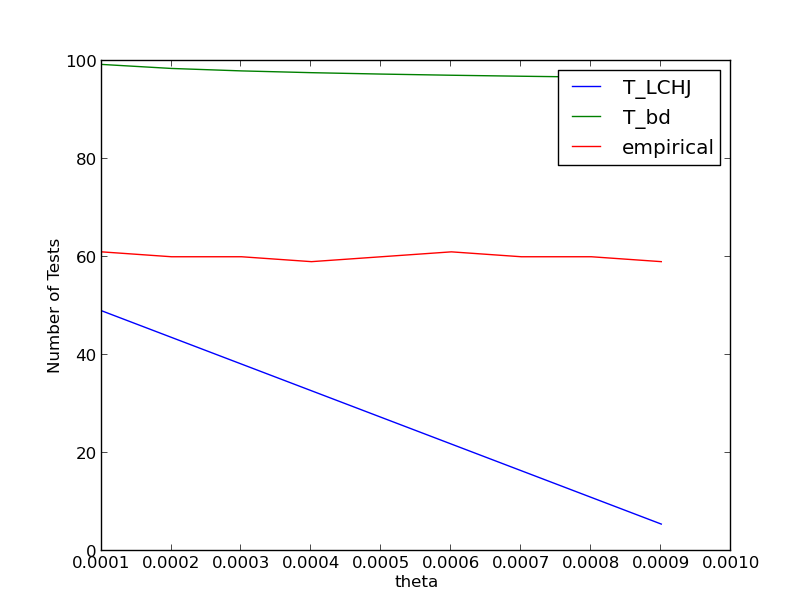
\includegraphics[width=0.5\textwidth]{ubvslb.png}
\caption{Theoretical lower and upper bounds and empirical Test frequencies as functions of \(\theta\)}
\label{ubvslb}
\end{figure}

Note that the Upper bound is not optimal and there still is some room for improvement. Note also that the lower bound degrades with \(\theta_i \). The lower bound (\(T_{LCHJ}\)) was generated according to theorem (\ref{thm:upper}). 

\begin{figure}[h]
\centering
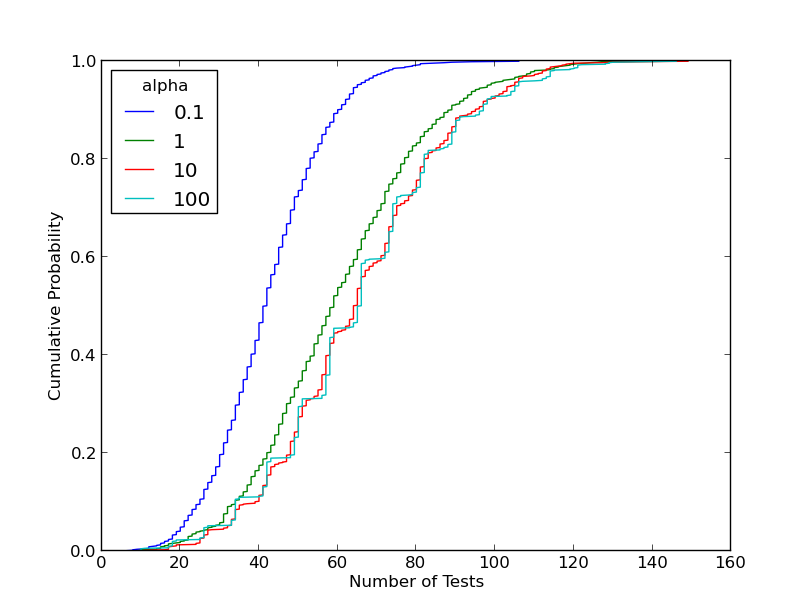
\includegraphics[width=0.5\textwidth]{variousalpha.png}
\caption{Cumulative distribution curves of the modified Hwang algorithm with fixed \(\theta = 0.0001\) and \(\alpha\) varying }
\label{testsvsalpha}
\end{figure}

\begin{figure}[h]
\centering
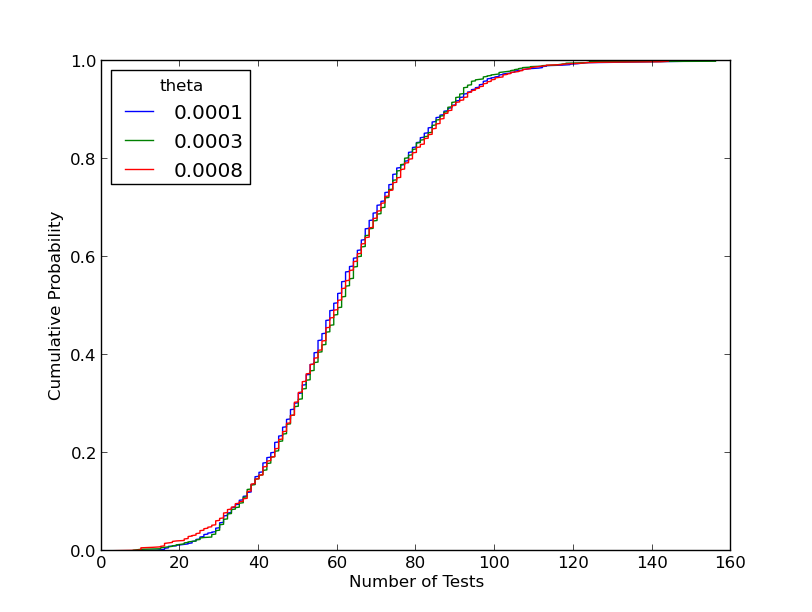
\includegraphics[width=0.5\textwidth]{nicegraphlaminar.png}
\caption{Cumulative distribution curves for fixed \(\alpha = 1\) and varying \(\theta\)}
\label{testsvstheta}
\end{figure}

Figures (\ref{testsvsalpha}) and (\ref{testsvstheta}) show that the performance is relatively insensitive to the cut-off \(\theta\), and more sensitive to the uniformity (or otherwise) of the probability distribution \(\vc{p}\). Heuristically, this is for because distributions which are highly concentrated on a few items algorithms can make substantial savings on the testing budget by testing those highly likely items first (which is captured in the bin structure of the above algorithm). 

The insensitivity to the cutoff \(\theta\) is due to items below \(\theta\) being overwhelmingly unlikely to be defective - which for small \(\theta\) means that few items (relative to the size of the problem) get discarded.

\section{Discussion}
%
We have introduced and analysed an algorithm for Probabilistic group testing which uses `just over' $H(\vc{U})$ tests to
recover all the defectives with high probability. Combined with a weak converse taken from \cite{li5}, this allows us to deduce that
the weak capacity of Probabilistic group testing is $C=1$.  
These results are illustrated by simulation.

For simplicity, this work has concentrated on establishing a bound $T_{\bd}$ in \eqref{eq:tbd} which has leading term $H(\vc{U})$,
and not on tightening bounds on the coefficient of $\mu$ in \eqref{eq:tbd}. For completeness, we mention that this coefficient
can be reduced from 3, under a simple further condition:

\begin{remark}
For some $c \leq 1/2$, we assume that all the $p_i \leq c$, and we alter the definition of `fullness' to assume that a set is
full if it has total probability less than $\alpha$. In this case, the term $P_{\setS} \log_2 P_{\setS}$ in \eqref{eq:tbds}
becomes $P_{\setS} \log_2 (\alpha + c)$, the bound in \eqref{eq:counting} becomes $\mu/\alpha$, and since
$\left( (1-p) \log_2 (1-p) \right)/p$ is decreasing in $p$, we can add a term $(1-c) \log_2 (1-c) $ to \eqref{eq:toopt}.
Overall, the coefficient of $\mu$ becomes $f(a,c) := \log_2 (\alpha + c) + 1 + 1/\alpha + (1-c) \log_2(1-c)$, which we can optimize over
$\alpha$. For example, if $c = 1/4$, taking $\alpha = 0.88824$, we obtain $f(a,c) = 2.00135$.
\end{remark}

It remains of interest to tighten the upper bound of Theorem \ref{thm:upper},
in order prove a strong converse, and hence confirm that the strong capacity is also equal to $1$.

In future work, we hope to explore more realistic models of defectivity, such as those where the defectivity of $U_i$ are not
necessarily independent, for example by imposing a Markov neighbourhood structure.

\section*{Acknowledgments}

This work was supported by the Engineering and Physical Sciences Research Council [grant number {\tt EP/I028153/1}]; Ofcom; and the University of Bristol. The authors would particularly like to thank Gary Clemo of Ofcom for useful discussions.

\bibliography{../../}
\end{document}



\backmatter

\fancyhead[LE]{\nouppercase{\leftmark}}
\fancyhead[RO]{\nouppercase{\rightmark}}

\bibliographystyle{jfm}
\addcontentsline{toc}{chapter}{Bibliography}

\end{document}